\documentclass[type=master]{thuthesis}
% 选项:
%   type=[bachelor|master|doctor|postdoctor], % 必选
%   secret,                                   % 可选
%   pifootnote,                               % 可选(建议打开)
%   openany|openright,                        % 可选,基本不用
%   arial,                                    % 可选,基本不用
%   arialtoc,                                 % 可选,基本不用
%   arialtitle                                % 可选,基本不用

% 所有其它可能用到的包都统一放到这里了,可以根据自己的实际添加或者删除。
\usepackage{thuthesis}
\usepackage{listings}
\usepackage{xcolor}

% 定义所有的图片文件在 figures 子目录下
\graphicspath{{figures/}}

% 可以在这里修改配置文件中的定义。导言区可以使用中文。
\def\myname{武斌}

\begin{document}

%%% 封面部分
\frontmatter
\thusetup{
  %******************************
  % 注意:
  %   1. 配置里面不要出现空行
  %   2. 不需要的配置信息可以删除
  %******************************
  %
  % 中国海洋大学研究生学位论文封面
  % 参考:中国海洋大学研究生学位论文书写格式20130307.doc
  % 为避免出现错误,下面保留[清华大学学位论文模板原有定义无需修改],
  % 请直接跳到后面[中国海洋大学学位论文模板部分请根据自己情况修改]。
  %
%%%%%%%%%%%%%%%%%%%%%%[清华大学学位论文模板原有定义无需修改]%%%%%%%%%%%%%%%%%%%%%%%
  %=====
  % 秘级
  %=====
  secretlevel={秘密},
  secretyear={10},
  %
  %=========
  % 中文信息
  %=========
  ctitle={清华大学学位论文 \LaTeX\ 模板\\使用示例文档 v\version},
  cdegree={工学硕士},
  cdepartment={计算机科学与技术系},
  cmajor={计算机科学与技术},
  cauthor={薛瑞尼},
  csupervisor={郑纬民教授},
  cassosupervisor={陈文光教授}, % 副指导老师
  ccosupervisor={某某某教授}, % 联合指导老师
  % 日期自动使用当前时间,若需指定按如下方式修改:
  % cdate={超新星纪元},
  %
  % 博士后专有部分
  cfirstdiscipline={计算机科学与技术},
  cseconddiscipline={系统结构},
  postdoctordate={2009年7月——2011年7月},
  id={编号}, % 可以留空: id={},
  udc={UDC}, % 可以留空
  catalognumber={分类号}, % 可以留空
  %
  %=========
  % 英文信息
  %=========
  etitle={An Introduction to \LaTeX{} Thesis Template of Tsinghua University v\version},
  % 这块比较复杂,需要分情况讨论:
  % 1. 学术型硕士
  %    edegree:必须为Master of Arts或Master of Science(注意大小写)
  %             “哲学、文学、历史学、法学、教育学、艺术学门类,公共管理学科
  %              填写Master of Arts,其它填写Master of Science”
  %    emajor:“获得一级学科授权的学科填写一级学科名称,其它填写二级学科名称”
  % 2. 专业型硕士
  %    edegree:“填写专业学位英文名称全称”
  %    emajor:“工程硕士填写工程领域,其它专业学位不填写此项”
  % 3. 学术型博士
  %    edegree:Doctor of Philosophy(注意大小写)
  %    emajor:“获得一级学科授权的学科填写一级学科名称,其它填写二级学科名称”
  % 4. 专业型博士
  %    edegree:“填写专业学位英文名称全称”
  %    emajor:不填写此项
  edegree={Doctor of Engineering},
  emajor={Computer Science and Technology},
  eauthor={Xue Ruini},
  esupervisor={Professor Zheng Weimin},
  eassosupervisor={Chen Wenguang},
  % 日期自动生成,若需指定按如下方式修改:
  % edate={December, 2005}
  %
  % 关键词用“英文逗号”分割
  ckeywords={\TeX, \LaTeX, CJK, 模板, 论文},
  ekeywords={\TeX, \LaTeX, CJK, template, thesis}
}

% 定义中英文摘要和关键字
\begin{cabstract}
  论文的摘要是对论文研究内容和成果的高度概括。摘要应对论文所研究的问题及其研究目
  的进行描述,对研究方法和过程进行简单介绍,对研究成果和所得结论进行概括。摘要应
  具有独立性和自明性,其内容应包含与论文全文同等量的主要信息。使读者即使不阅读全
  文,通过摘要就能了解论文的总体内容和主要成果。

  论文摘要的书写应力求精确、简明。切忌写成对论文书写内容进行提要的形式,尤其要避
  免“第 1 章……;第 2 章……;……”这种或类似的陈述方式。

  本文介绍清华大学论文模板 \thuthesis{} 的使用方法。本模板符合学校的本科、硕士、
  博士论文格式要求。

  本文的创新点主要有:
  \begin{itemize}
    \item 用例子来解释模板的使用方法;
    \item 用废话来填充无关紧要的部分;
    \item 一边学习摸索一边编写新代码。
  \end{itemize}

  关键词是为了文献标引工作、用以表示全文主要内容信息的单词或术语。关键词不超过 5
  个,每个关键词中间用分号分隔。(模板作者注:关键词分隔符不用考虑,模板会自动处
  理。英文关键词同理。)
\end{cabstract}

% 如果习惯关键字跟在摘要文字后面,可以用直接命令来设置,如下:
% \ckeywords{\TeX, \LaTeX, CJK, 模板, 论文}

\begin{eabstract}
   An abstract of a dissertation is a summary and extraction of research work
   and contributions. Included in an abstract should be description of research
   topic and research objective, brief introduction to methodology and research
   process, and summarization of conclusion and contributions of the
   research. An abstract should be characterized by independence and clarity and
   carry identical information with the dissertation. It should be such that the
   general idea and major contributions of the dissertation are conveyed without
   reading the dissertation.

   An abstract should be concise and to the point. It is a misunderstanding to
   make an abstract an outline of the dissertation and words ``the first
   chapter'', ``the second chapter'' and the like should be avoided in the
   abstract.

   Key words are terms used in a dissertation for indexing, reflecting core
   information of the dissertation. An abstract may contain a maximum of 5 key
   words, with semi-colons used in between to separate one another.
\end{eabstract}

% \ekeywords{\TeX, \LaTeX, CJK, template, thesis}
%%%%%%%%%%%%%%%%%%%%%%%%%%%%%%%%%%%%%%%%%%%%%%%%%%%%%%%%%%%%%%%%%%%%%%%%%%%%%%%%

%%%%%%%%%%%%%%%%%%[中国海洋大学学位论文模板部分请根据自己情况修改]%%%%%%%%%%%%%%%%%%%
% 中国海洋大学研究生学位论文封面
% 必须填写的内容包括(其他最好不要修改):
%   分类号、密级、UDC
%   论文中文题目、作者中文姓名
%   论文答辩时间
%   封面感谢语
%   论文英文题目
%   中文摘要、中文关键词
%   英文摘要、英文关键词
%
%%%%%[自定义]%%%%%
\newcommand{\fenleihao}{}%分类号
\newcommand{\miji}{}%密级
                    % 绝密$\bigstar$20年
                    % 机密$\bigstar$10年
                    % 秘密$\bigstar$5年
\newcommand{\UDC}{}%UDC
\newcommand{\oucctitle}{基于Spring MVC架构的WEB平台系统优化策略研究}%论文中文题目
\ctitle{基于Spring MVC架构的WEB平台系统优化策略研究}%必须修改因为页眉中用到
\cauthor{武斌}%可以选择修改因为仅在 pdf 文档信息中用到
\cdegree{工学硕士}%可以选择修改因为仅在 pdf 文档信息中用到
\ckeywords{\TeX, \LaTeX, CJK, 模板, 论文}%可以选择修改因为仅在 pdf 文档信息中用到
\newcommand{\ouccauthor}{武斌}%作者中文姓名
%\newcommand{\ouccsupervisor}{姬光荣教授}%作者导师中文姓名
%\newcommand{\ouccdegree}{博\hspace{1em}士}%作者申请学位级别
%\newcommand{\ouccmajor}{海洋信息探测与处理}%作者专业名称
%\newcommand{\ouccdateday}{\CJKdigits{\the\year}年\CJKnumber{\the\month}月\CJKnumber{\the\day}日}
%\newcommand{\ouccdate}{\CJKdigits{\the\year}年\CJKnumber{\the\month}月}
\newcommand{\oucdatedefense}{2017年05月28日}%论文答辩时间
%\newcommand{\oucdatedegree}{2009年6月}%学位授予时间
\newcommand{\oucgratitude}{谨以此论文献给我的导师和亲人!}%封面感谢语
\newcommand{\oucetitle}{Research on Web Platform System Optimization Strategy Based on Spring MVC Framework}%论文英文题目
%\newcommand{\ouceauthor}{Haiyong Zheng}%作者英文姓名
\newcommand{\oucthesis}{\textsc{OUCThesis}}
%%%%%默认自定义命令%%%%%
% 空下划线定义
\newcommand{\oucblankunderline}[1]{\rule[-2pt]{#1}{.7pt}}
\newcommand{\oucunderline}[2]{\underline{\hskip #1 #2 \hskip#1}}

% 论文封面第一页
%%不需要改动%%
\vspace*{5cm}
{\xiaoer\heiti\oucgratitude

\begin{flushright}
---\hspace*{-2mm}---\hspace*{-2mm}---\hspace*{-2mm}---\hspace*{-2mm}---\hspace*{-2mm}---\hspace*{-2mm}---\hspace*{-2mm}---\hspace*{-2mm}---\hspace*{-2mm}---~\ouccauthor
\end{flushright}
}

\newpage

% 论文封面第二页
%%不需要改动%%
\vspace*{1cm}
\begin{center}
  {\xiaoer\heiti\oucctitle}
\end{center}
\vspace{10.7cm}
{\normalsize\songti
\begin{flushright}
{\renewcommand{\arraystretch}{1.3}
  \begin{tabular}{r@{}l}
    学位论文答辩日期:~ & \oucunderline{1.8em}{\oucdatedefense} \\
    指导教师签字:~ & \oucblankunderline{5cm} \\
    答辩委员会成员签字:~ & \oucblankunderline{5cm} \\
    ~ & \oucblankunderline{5cm} \\
    ~ & \oucblankunderline{5cm} \\
    ~ & \oucblankunderline{5cm} \\
    ~ & \oucblankunderline{5cm} \\
    ~ & \oucblankunderline{5cm} \\
    ~ & \oucblankunderline{5cm} \\
  \end{tabular}
}
\end{flushright}
}

\newpage

% 论文封面第三页
%%不需要改动%%
\vspace*{1cm}
\begin{center}
  {\xiaosan\heiti 独\hspace{1em}创\hspace{1em}声\hspace{1em}明}
\end{center}
\par{\normalsize\songti\parindent2em
本人声明所呈交的学位论文是本人在导师指导下进行的研究工作及取得的研究成果。据我所知,除了文中特别加以标注和致谢的地方外,论文中不包含其他人已经发表或撰写过的研究成果,也不包含未获得~\oucblankunderline{7cm}(注:如没有其他需要特别声明的,本栏可空)或其他教育机构的学位或证书使用过的材料。与我一同工作的同志对本研究所做的任何贡献均已在论文中作了明确的说明并表示谢意。
}
\vskip1.5cm
\begin{flushright}{\normalsize\songti
  学位论文作者签名:\hskip2cm 签字日期:\hskip1cm 年 \hskip0.7cm 月\hskip0.7cm 日}
\end{flushright}
\vskip.5cm
{\setlength{\unitlength}{0.1\textwidth}
  \begin{picture}(10, 0.1)
    \multiput(0,0)(0.2, 0){50}{\rule{0.15\unitlength}{.5pt}}
  \end{picture}}
\vskip1cm
\begin{center}
  {\xiaosan\heiti 学位论文版权使用授权书}
\end{center}
\par{\normalsize\songti\parindent2em
本学位论文作者完全了解学校有关保留、使用学位论文的规定,并同意以下事项:
\begin{enumerate}
\item 学校有权保留并向国家有关部门或机构送交论文的复印件和磁盘,允许论文被查阅和借阅。
\item 学校可以将学位论文的全部或部分内容编入有关数据库进行检索,可以采用影印、缩印或扫描等复制手段保存、汇编学位论文。同时授权清华大学“中国学术期刊(光盘版)电子杂志社”用于出版和编入CNKI《中国知识资源总库》,授权中国科学技术信息研究所将本学位论文收录到《中国学位论文全文数据库》。
\end{enumerate}
(保密的学位论文在解密后适用本授权书)
}
\vskip1.5cm
{\parindent0pt\normalsize\songti
学位论文作者签名:\hskip4.2cm\relax%
导师签字:\relax\hspace*{1.2cm}\\
签字日期:\hskip1cm 年\hskip0.7cm 月\hskip0.7cm 日\relax\hfill%
签字日期:\hskip1cm 年\hskip0.7cm 月\hskip0.7cm 日\relax\hspace*{1.2cm}}

\newpage

\pagestyle{plain}
\clearpage\pagenumbering{roman}

% 中文摘要
%%[需要填写:中文摘要、中文关键词]%%
\begin{center}
  {\sanhao[1.5]\heiti\oucctitle\\\vskip7pt 摘\hspace{1em}要}
\end{center}
{\normalsize\songti

  \indent
  近几年,随着中国经济的不断发展以及中国互联网整体水平的不断提高,虚拟
  经济在中国的经济发展中扮演着越来越重要的作用,WEB应用作为虚拟经济的
  主要呈现方式也获得了非常大的发展。越来越多面向不同消费群体的WEB应用
  被设计和开发出来为消费者提供各种的服务。

  随着Internet网的不断告诉发展,人们对于WEB应用的需要不再基于可用性那
  么简单,应用的用户体验越来越被重视~\cite{李梦2016基于前端的}。然而,
  随着用户数量的不断增加,WEB服务器的信息量和访问量成几何数级的增长,网
  络拥塞和服务超载日益成为开发人员必须面对的严峻问题。

  因此在WEB应用的开发过程中,开发人员不但需要在代码的书写上要进行不断优化,
  降低代码的错误率和提升代码的执行效率外,而且要将很大的精力放到服务器性能
  优化方面,通过调整WEB服务器的运行参数提升服务器的响应效率、优化缓存机制
  提升数据的存取效率,设计负载均衡方案实现应用服务器的负载均衡,开发数据库
  的主从复制和延时复制等策略保证数据的稳定性以及编写监控脚本实现服务的实施
  监控等措施来提升应用的体验和增强系统的安全性。

  本文的创新点主要有:
  \begin{itemize}
    \item 通过Jenkins实现WEB应用的自动构建和部署,提升了WEB应用的稳定性,降低代码错误率;
    \item 基于Couchbase缓存机制,加快了应用的数据读取,降低了系统的响应时间;
    \item 通过Docker容器编排技术,方便的实现服务集群节点的扩展,增强了系统的安全性,实现了统一管理和维护;
    \item 通过负载均衡,降低了应用服务器和数据服务器的压力,提升了用户的体验;
    \item 充分利用API实现监控脚本,实现了应用的实时监控,很大程度上减少了发现问题和故障处理的时间;
  \end{itemize}

}
\vskip12bp
{\xiaosi\heiti\noindent
关键词:\hskip1em Spring MVC框架应用开发; WEB应用性能优化; 数据库性能优化; 服务监控及应对方案; }

\newpage

% 英文摘要
%%[需要填写:英文摘要、英文关键词]%%
\begin{center}
  {\sanhao[1.5]\heiti\oucetitle\\\vskip7pt Abstract}
\end{center}
{\normalsize\songti

   In recent years, with the continuous development of China's economy and the continuous improvement of the overall level of China's Internet, virtual economy plays an increasingly important role in China's economic development, WEB application as a virtual economy is also the main presentation of the very Big development. More and more for different consumer groups of WEB applications are designed and developed to provide consumers with a variety of services.

   With the continuous development of the Internet to tell the people, the need for WEB applications is no longer based on usability so simple, application user experience more and more attention. However, with the increase of the number of users, the amount of information and the number of visits of the WEB server grows geometrically. Network congestion and service overload are increasingly becoming the serious problem that the developers must face.

   Therefore, in the WEB application development process, developers need to not only write code on the continuous optimization to reduce the code error rate and improve the efficiency of the code, but also to a lot of energy into the server performance optimization, By adjusting the operating parameters of the WEB server to improve the response efficiency of the server and optimize the cache mechanism to improve the efficiency of data access, the design load balancing solution to achieve the application server load balancing, database replication master and slave replication and delay replication strategy to ensure data stability As well as the preparation of monitoring scripts to achieve the implementation of service monitoring and other measures to enhance the application experience and enhance the security of the system.

   The innovation of this paper:
  \begin{itemize}
    \item Through Jenkins to realize the automatic construction and deployment of WEB applications to enhance the stability and reduce code error rate;
    \item Through Couchbase cache mechanism to speed up the data read of application, reducing the system response time;
    \item Through Docker container scheduling technology to facilitate the expansion of service cluster nodes to enhance the security of the system to achieve a unified management and maintenance;
    \item Reduces stress on application servers and data servers through load balancing and improves user experience;
    \item Make full use of API to achieve the monitoring script to achieve the application of real-time monitoring, to a large extent reduce the discovery of problems and troubleshooting time;
  \end{itemize}
}
\vskip12bp
{\xiaosi\heiti\noindent
\textbf{Keywords:\enskip WEB Aplication Development Based on Spring MVC; WEB Application Performance Optimization; Database Performance Optimization; Service Monitoring and Response Strategies}}
%%%%%%%%%%%%%%%%%%%%%%%%%%%%%%%%%%%%%%%%%%%%%%%%%%%%%%%%%%%%%%%%%%%%%%%%%%%%%%%%
% 如果使用授权说明扫描页,将可选参数中指定为扫描得到的 PDF 文件名,例如:
% \makecover[scan-auth.pdf]
%\makecover

%% 目录
\tableofcontents

%% 符号对照表
\begin{denotation}[3cm]
\item[Internet] 互联网
\item[SLB] 服务器负载均衡 (Server Load Balancing)
\item[cluster] 集群
\item[Itanium] 安腾
\item[SMP] 对称多处理
\item[API] 应用程序编程接口
\item[PI] 聚酰亚胺
\item[MPI] 聚酰亚胺模型化合物,N-苯基邻苯酰亚胺
\item[PBI] 聚苯并咪唑
\item[MPBI] 聚苯并咪唑模型化合物,N-苯基苯并咪唑
\item[PY] 聚吡咙
\item[PMDA-BDA]	均苯四酸二酐与联苯四胺合成的聚吡咙薄膜
\item[$\Delta G$] 活化自由能 (Activation Free Energy)
\item[$\chi$] 传输系数 (Transmission Coefficient)
\item[$E$] 能量
\item[$m$] 质量
\item[$c$] 光速
\item[$P$] 概率
\item[$T$] 时间
\item[$v$] 速度
\end{denotation}



%%% 正文部分
\mainmatter
%% 代码样式
\lstset{
columns=fixed,
numbers=left,                                        % 在左侧显示行号
escapeinside=``,   % 设定`....`之内为逃逸部分,这部分内容将按照正常的LaTeX代码编译
breaklines=true,    % 设定LaTeX对过长的代码行进行自动换行
backgroundcolor=\color{lightgray!40!white},    % 设定代码区底色为浅灰色,lightgray!40!white是指lightgray、white两种颜色四六开混合得到的颜色,这两种颜色以及\color{}命令由xcolor宏包提供
frame=none, % 设定代码区不加框
extendedchars=false, % 解决代码跨页时,章节标题、页眉页脚的汉字无法正常显示的问题
keywordstyle=\color{blue!70}\bfseries,    % 设定相应语言中关键字突出显示方式为蓝色、加粗,实现语法高亮
basicstyle=\ttfamily,    % 设定代码的基本字体为等宽字体(类似于Courier)
%commentstyle=\color{red!50!green!50!blue!50},
numberstyle=\footnotesize\color{darkgray},           % 设定行号格式
commentstyle=\ttfamily\color{green!40!black},    % 设定注释部分字体为等宽字体,用深绿色显示
rulesepcolor=\color{red!20!green!20!blue!20},
showstringspaces=false,    % 设定代码中字符串的空格正常显示,而不是显示为特殊字符“␣”
stringstyle=\rmfamily\slshape\color[RGB]{128,0,0},   % 设置字符串格式
}
\chapter{绪论}
\label{cha:introduction}
\section{论文研究背景及意义}
随着信息技术的不断发展,21世纪我们已经进入了一个“信息爆炸”的社会,而且在近几年我们的社会几乎进入互联网时代后,社会中的每个人每天接收到的咨询和信息以及各种各样的互联网产品同互联网发展的初期相比,超出了太多太多。~\cite{林薇2015基于}。另外,我国的互联网技术在近十几年内不断的发展,开发WEB产品的人力成本和技术成本不断降低,用户对于 WEB 应用的需求\cite{邵志强2015跨媒体检索平台}不再满足于通过缓慢的加载和复杂的操作获取资讯~\cite{贺海梁2012基于},
许多的创业者希望通过开发一个WEB应用实现自己创业梦想的时代已经无法获得投资人的青睐。而且,由于近几年WEB信息泄露的新闻不断进入消费者的视野,用户对于WEB应用的安全性体验也提出了更高的要求。

随着互联网技术进一步普及,基于模型-视图-控制器
(Model-View-Controller, MVC)模式的WEB应用程序~\cite{张2010基于}被广大开发者所使用,目前主流的WEB应用程序均在使用此框架。使用MVC框架,可以将WEB应用进行清晰的分层开发,前端开发人员主要负责页面的呈现方式和用户体验,后台人员则主要负责应用的逻辑实现以及数据结构的搭建,极大的降低了研发成本。

随着信息化的进一步普及,数据库的使用越来越广泛,数据成为一个应用甚至也个企业最重要的价值体现,越来越多的企业发展离不开数据库。因此数据库的稳定性和安全性也称为很多企业研发的重点。通过设计数据的管理和使用机制,在提高数据库使用效率的同时,保障数据的完整性和安全性是企业运维人员的在运维过程中的重要任务。

除此之外,如何实现WEB应用的高可用性和分布式服务也是保障用户体验的一个很重要的部分,通过设计基于应用和服务器的不同层级不同纬度的优化策略,提升应用的高可用性也是在WEB应用开发中必须要注意的。

\section{国内外研究现状}
从上世纪九十年代开始,计算机技术和Internet互联网技术开始迅速发展, 随着这些技术的不断发展,在互联网络中网络信息的存储量级和访问数量都是以几何数级进行增长,随之而来导致的问题就是网络访问的拥塞问题和网络服务的超载运行~\cite{王霜2004web}。

2006年新华网被黑事件、2010年的百度域名劫持时间、2011年的CSDN用户数据泄漏事件以及2015年网易邮箱密码泄漏事件等事件无不说明系统优化的作用和意义。

目前大部分互联网产品在开始发展的阶段都重视了产品的设计和功能,然而在产品的稳定性和安全性方面却考虑不足,这在一定程度上增加了互联网产品在推广过程中潜在的风险。因此,在开发互联网产品的同时,通过一系列的优化策略,提升应用的体验,增强应用的稳定性和安全性必须得到充分的认识。

\section{论文主要研究内容}
\subsection{论文主要工作内容}
本篇论文通过在满足本人参与的WEB应用正常运行的基础上,通过应用、数据和服务等不同维度的的优化实践研究基于Spring MVC架构WEB应用的系统优化策略。首先通过搭建基于Spring MVC的WEB测试应用,在实际用户使用的过程中通过不断开发和调整系统的优化策略,提升应用的用户体验和应用的稳定性,探索行之有效的系统优化策略。

本文的研究对象主要有以下内容:

(1) 对Jenkins持续集成环境研究。自动化部署和代码检测是保证基于WEB的应用产品质量的一个重要环节,通过研究部署Jenkins集成测试环境,对编写的代码进行版本控制、自动化构建和代码测试,研究持续集成方案对于WEB应用系统优化策略的影响。

(2) 对Couchbase缓存机制进行研究。目前大多数的WEB应用对于缓存性能的优化还没有足够的重视,通过开发针对WEB应用的Couchbase缓存系统,研究Couchbase的缓存机制测试有效的缓存机制对于系统性能提升和用户体验的影响,探索可用的系统优化策略。

(3) 对Docker容器编排技术进行研究。随着用户的不断增加,单一节点的WEB应用或数据库应用已经无法满足用户的需求,如何快速的部署新的应用节点提升应用性能成为开发者关注的问题。通过构建基于Docker容器编排技术的应用容器,在新的服务器快速部署新的应用,并加入到应用集群中去,探索Docker机制对于系统优化策略的影响。

(4) 对数据库的主从复制进行研究。随着应用的发展,数据逐渐成为应用最有价值的部分,如何更好的保证数据的完整性以及安全性在应用的维护过程中日益重要。通过研究数据库的主从复制和延时复制方案,探索数据库优化对于系统安全性优化的策略。

(5) 对基于API的监控和应急措施方案进行研究。随着服务节点的不断增加,服务的高可用和服务的健康性检查时WEB应用的运维人员在维护过程中必须要注意的方面。通过开发基于API的服务器、服务监控系统以及基于API的应急处理系统研究API操作对于系统的快速检测和快速恢复的影响。

(6) 其他方面,研究WEB应用的搭建过程、Tomcat的相关配置、负载均衡以及阿里云的相关配置研究WEB应用和服务器自身优化对于系统性能的影响。

\subsection{论文目标}
本论文致力于分析目前很多WEB应用开发过程中存在的问题和不完善的地方,并探索WEB应用性能和服务器性能的优化方案。

在Linux平台上,使用JAVA语言和MySQL数据搭建一个基于Spring MVC架构的WEB应用,通过Tomcat实现应用的访问和测试,通过设计不同的优化方案对WEB进行测试,研究在实际应用中有价值的优化策略。

系统性能优化策略研究主要包含应用层面、数据层面和服务器层面三个层面。在应用层面,通过持续集成、代码审核实现应用的稳定性和安全性。在数据库层面,通过多数据库主从复制、负载均衡和备份恢复等策略实现数据的高可用和稳定性。在服务器层面,通过对服务的监控和服务器的监控、服务器间负载均衡的配置、基于API的自动化failover等策略保障服务的正常运行和高负载应对。
\section{论文组织结构}
基于Spring MVC架构WEB应用的系统优化策略的研究是按照计划逐步完成的,本人将此研究分为六个部分:

第一章:绪论。本章主要介绍WEB应用开发的现状和系统优化策略研究的意义,明确了在WEB应用开发过程中对于应用和服务器进行优化的必要性和重要性。除此之外,本章还介绍了论文主研究和实验的主要内容、论文的目标、论文创新点以及本篇论文的主要结构。

第二章:WEB应用开发介绍。本章主要介绍了前端和后端的开发框架和开发流程以及数据库的搭建过程。然后介绍了Tomcat的配置过程。之后介绍了Jenkins持续集成环境的搭建和使用过程。

第三章:应用性能优化介绍。本章主要介绍了在WEB应用性能优化方面册主要方法和策略,主要包括Couchbase缓存优化,Tomcat高性能Apr配置,Docker分布式优化以及SLB负载均衡优化等方面。同时对应用的安全性和稳定性进行了分析。

第四章:数据优化。本章主要介绍了MySQL数据库在设计和开发过程的优化策略,主要包括基于数据稳定性的复制方案,基于高可用的负载均衡方案,基于数据完整性的备份和恢复方案。同时总结了出现问题时的解决方案。

第五章:服务监控与应急措施优化。本章主要介绍了服务器层面的优化策略,主要包括多服务器的心跳监听服务配置,服务性能的监控脚本实现,基于API的应急措施处置以及服务器安全性配置等方面的优化策略。同时总结了多种方案整合使用的策略。

第六章:总结与展望。本章主要总结了不同优化策略对于系统性能的影响以及在研究过程中获得的经验,并对优化策略的进一步研究做了简单的展望。
\chapter{WEB应用开发及持续集成}
\label{cha:web}
本论文的研究目的是对于开发的WEB应用进行应用、数据库和服务器层级进行优化,通过对比不同优化策略对于系统性能提升的影响研究一套可行的系统优化策略。为了实现优化的目的,首先需要创建一个WEB应用或者对现有的应用进行优化,本人在研究生期间,参与了海信集团智能商用公司的小微商户平台系统的开发,主要工作是后台开发和服务器运维工作,因此本论文将基于参与的小微商户WEB平台进行系统优化策略的研究。

在优化之前,首先需要描述作为优化原型的小微商户WEB平台的平台的开发框架以及应用部署流程。

% 本章首先介绍WEB应用开发的主要程序语言,然后对Spring MVC框架进行了详细的介绍。同时,对各种技术的应用反问做了初步的探讨,为后文系统性能优化工作做好理论工具上的准备。
% \section{应用开发语言}
% 目前WEB应用开发主要分为前端开发和后端开发,其中前端开发以HTML和JavaScript结合为主,后端开发语言则比较多,主流的有C语言、PHP语言、JAVA语言以及Python语言等语言,不同语言之间的作用和特点都不同,但在提高系统稳定性和系统兼容性方面JAVA语言更有优势~\cite{suzumura2008performance}。
% \subsection{JAVA语言}
% \subsubsection{JAVA语言产生及发展}
% JAVA语言是在20世纪90年代产生的,任职于太阳微系统的詹姆斯·高斯林等人于1990年代初开发Java语言的雏形,最初被命名为Oak,目标设置在家用电器等小型系统的程序语言,应用在电视机、电话、闹钟、烤面包机等家用电器的控制和通信~\cite{byous1998java}。由于这些智能化家电的市场需求没有预期的高,Sun公司放弃了该项计划。随着1990年代互联网的发展,Sun公司看见Oak在互联网上应用的前景,于是改造了Oak,于1995年5月以Java的名称正式发布。Java伴随着互联网的迅猛发展而发展,逐渐成为重要的网络编程语言~\cite{java维基百科}。

% 在所有的编程语言中,应用最广泛的莫过于JAVA语言,该语言在面向对象的程序开发中一直有着突出的表现。因此在最近10几年间,JAVA语言一直保持在编程语言排行的前两名,参见图~\ref{fig:tiobe}。
% \begin{figure}[H] % use float package if you want it here
%   \centering
%   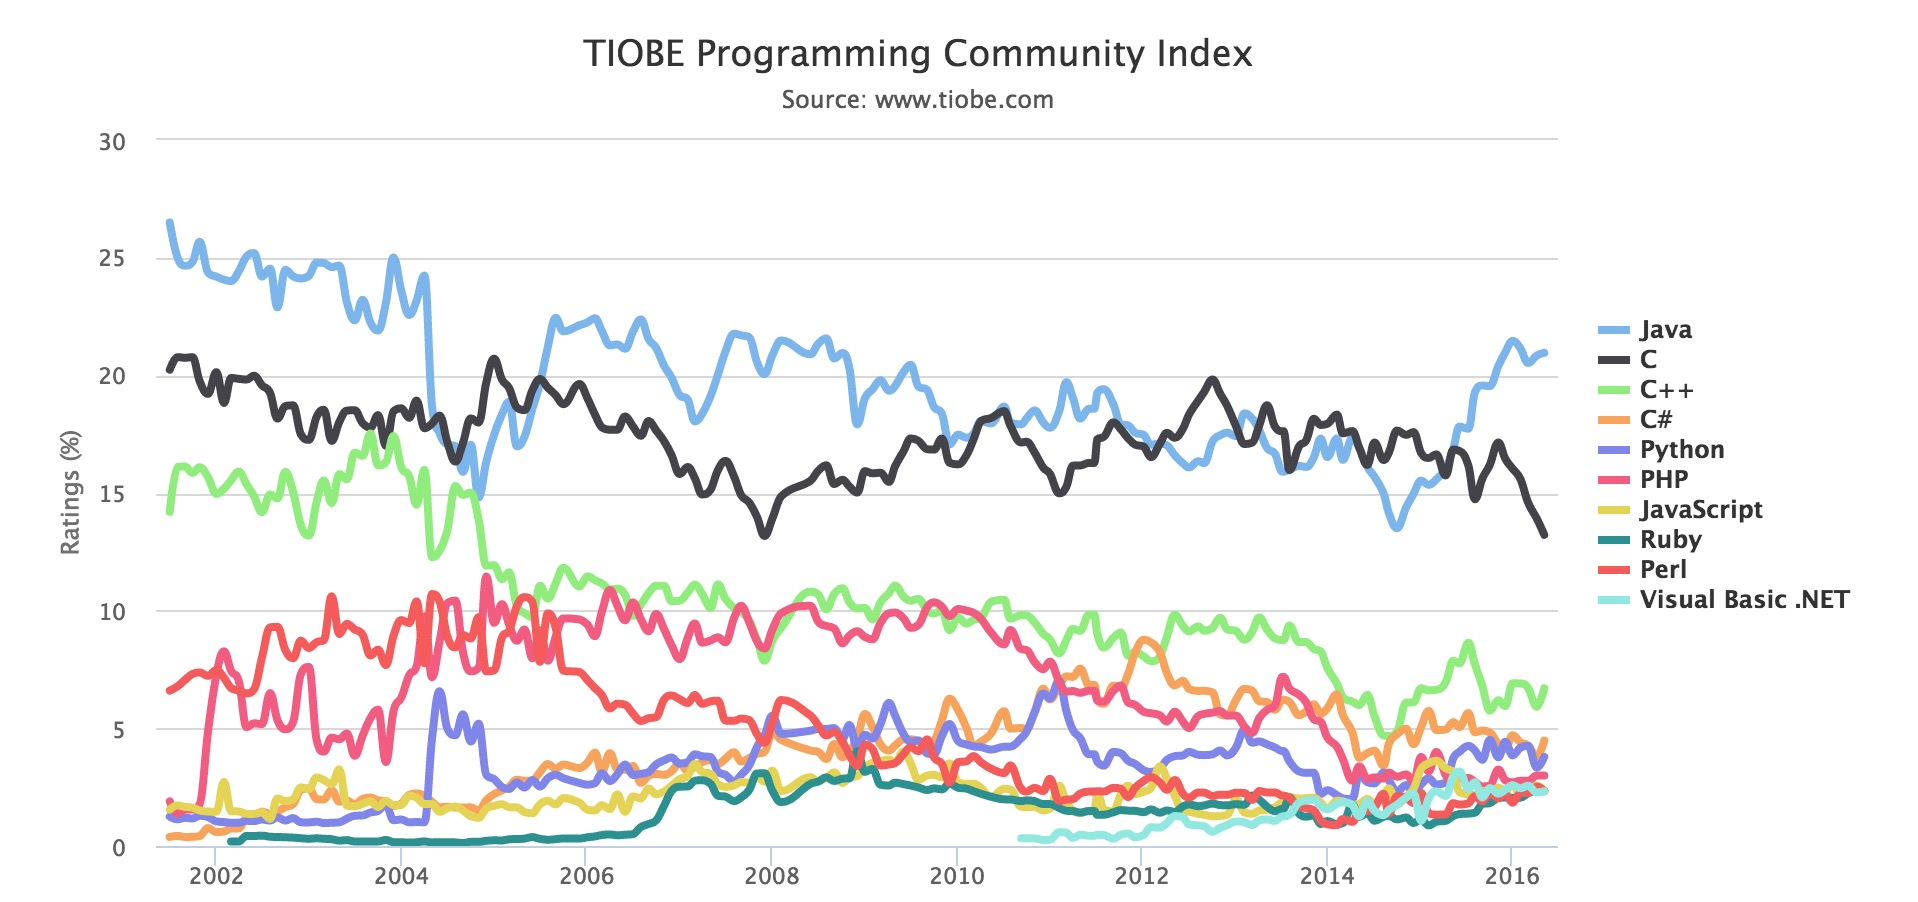
\includegraphics[width=6in]{chap02/1-TIOBE}
%   \caption{编程语言近年排行}
%   \label{fig:tiobe}
% \end{figure}
% \subsubsection{JAVA语言特点}
% 因特网的普及推动了JAVA语言的发展,同时JAVA语言在网页制作上的应用也丰富了因特网的内容。两者可谓是相辅相成、相互促进。JAVA语言的特点如表\ref{tab:java-1}。
% \begin{table}[htb]
%   \centering
%   \begin{minipage}[t]{0.8\linewidth} % 如果想在表格中使用脚注,minipage是个不错的办法
%   \caption[模板文件]{模板文件。如果表格的标题很长,那么在表格索引中就会很不美
%     观,所以要像 chapter 那样在前面用中括号写一个简短的标题。这个标题会出现在索
%     引中。}
%   \label{tab:java-1}
%     \begin{tabularx}{\linewidth}{lX}
%       \toprule[1.5pt]
%       {\heiti 特点} & {\heiti 描述} \\\midrule[1pt]
%       可移植性 & 能移植于不同的使用平台,扩大了系统的使用范围 \\
%       面向对象 & 集成了C++的优点,并且在面向对象方面有新的扩展 \\
%       多线程 & 可以让多个不同处理器同时进行工作,是数据库系统开发的最佳选择 \\
%       分布式 & 在处理TCP等协议的同时也支持网络编程\\
%       \bottomrule[1.5pt]
%     \end{tabularx}
%   \end{minipage}
% \end{table}


\section{Spring MVC开发框架}

Spring MVC 开发框架是一种针对Java语言开发的WEB系统架构,该框架的设计理念是的开发的系统整体进行分解,通过不同的方式对分解后的工作进行处理,以更加专业的技术解决具体的问题,最中在不同的模块中通过调用实现系统的整体呈现,通过这种方法系统的耦合度同其他的框架如Struts相比大大的降低。\cite{林薇2015基于}。
% \subsection{Spring MVC 架构的特点}
% Spring MVC 架构不同于传统的体系架构,在其发展的过程中吸收其他系统的特点,如支持Userful风格,灵活的本地化等。这些特征保证了Spring MVC框架在发展过程中,更加受到开发者的青睐。同时,吸收了前人的经验以后,Spring MVC框架也具备专属的特点,比如用Spring MVC框架设计的WEB系统其耦合度较低,系统总体表现出简洁明了的风格,这样用户就能更快捷的掌握数据库系统的操作~\cite{林薇2015基于}。

% Spring MVC框架是在Spring框架的基础上发展起来的,因此Spring MVC框架集成了Spring 框架的所有功能,而且两者在相互继承方面表现出很好的融合性。这一特点给系统开发带来了很多方便。除此之外,Spring MVC模型在图形兼容性和数据验证的灵活性上都有先天的优势。正式因为这些特点,使Spring MVC模型在实际应用中发挥出巨大的优势,同时也在程序员中受到青睐。本文的WEB应用就是建立在该框架之上的\cite{林薇2015基于}。
\subsection{Spring MVC 框架处理流程}

本框架是一个基于用户请求的系统架构。框架的处理过程参见图~\ref{fig:mvc},图形反映了一个简单的从用户请求开始到获得响应的过程。

\begin{figure}[H] % use float package if you want it here
  \centering
  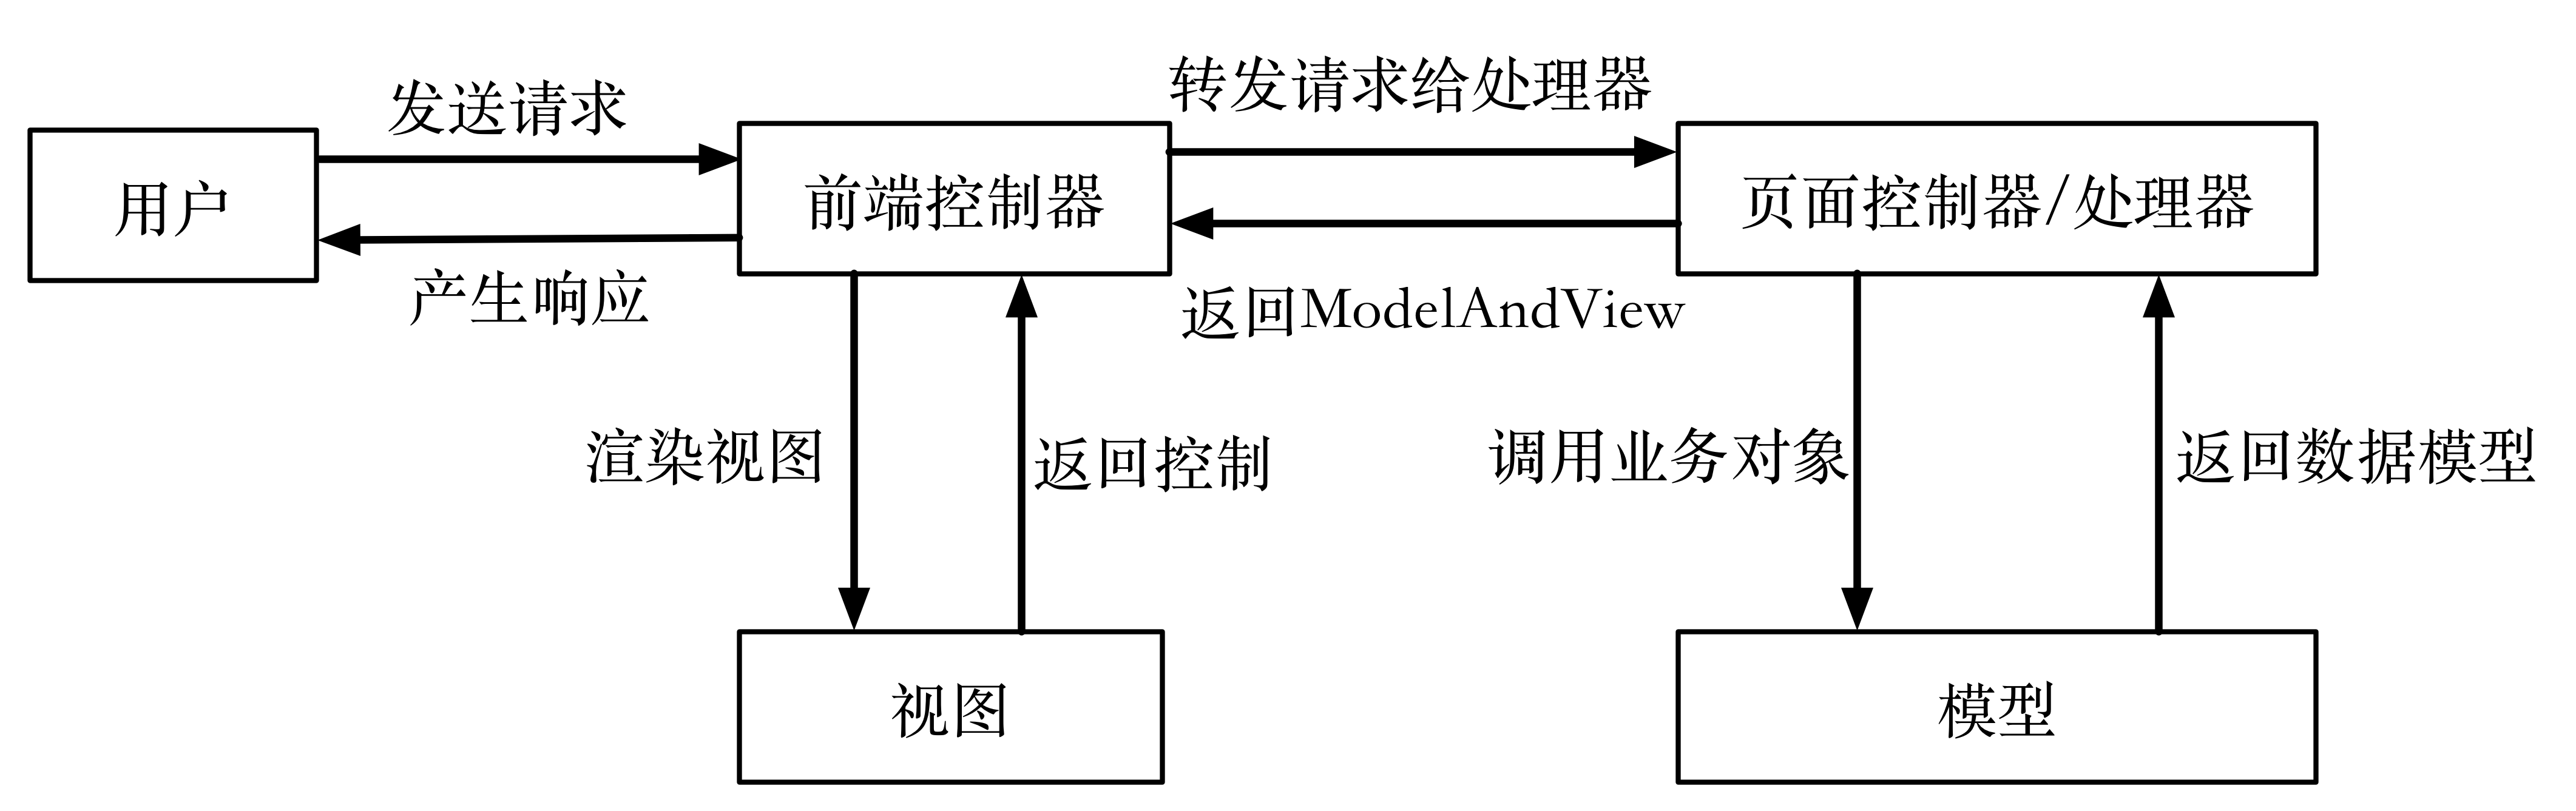
\includegraphics[width=6in]{chap02/mvc}
  \caption{Spring MVC请求响应过程}
  \label{fig:mvc}
\end{figure}

通过图可以看出,首先需要用户发送请求到框架的前端控制器,前端控制器接收到用户请求后会对用户的请求内容进行分析,获取到请求的控制器地址和请求参数,根据请求地址将用户请求转发到对应的后端控制器即处理器;处理器在接收到请求的参数之后开始调用后台的业务对象对请求进行分析和处理,在处理过程中会通过模型对存在数据库中的数据进行增、删、改、查的操作,处理完毕后将最新的数据返回给处理器;在请求的处理工作完成返回给前端控制器,之后对需要显示的结果进行视图渲染生成显示页面,展示给用户,对用户的请求产生了响应\cite{李守振2006web}。

\subsection{Spring MVC体系的三层架构}
Spring MVC开发框架的架构主要体现在MVC(Model View Controller),它是模型(M)、视图(V)和控制(C)三个英文单词的首字母缩写,根据字面意思我们也可以本系统的架构分为模型层(数据访问层)、视图层和控制层三层。

\begin{enumerate}

\item 视图层。主要负责前端页面的用户请求,将用户请求按照URL Mapping方式映射到相对应的控制器,通过分析用户请求,Spring可以自动的去寻找响应该请求的控制类,当控制类处理完请求后会将请求的结果以用户指定方式显示在前端页面上。

\item 控制层。 控制层是架构中承上启下的一层,这一层的作用是接受视图层传来的用户请求,然后针对请求设计实现用户请求的方法,需要用到数据的则会通过模型层获取数据结果,经过方法的处理获得用户请求的结果,并且将结果返回视图层。

\item 模型层,也可以成为数据访问层。这一层的作用主要是实现数据的访问方法和数据的返回方法,通过配置数据模型访问数据库并且获得需要的数据,将数据返回给控制层。

\end{enumerate}

以上的Spring MVC三层架构体系在很大程度上根据开发需求实现了业务的剥离,解决了开发过程中的开发资源和业务资源混乱的问题,而且降低了系统的耦合度。

\section{应用开发工具}

在开发基于 Spring MVC 的 WEB 应用过程中,需要用到的基础编程语言是 JAVA,系统的架构采用的 MVC 三层架构。但是在架构之外,程序本身的开发对于开发人员也非常重要,因此通过选择和使用一些比较好用的软件和工具,对于缩短开发周期提升开发效率来说非常重要。

\subsection{IntelliJ IDEA}

IntelliJ IDEA 是一款 Java 集中开发环境工具软件,由捷克软件公司 JetBrains 发布和维护~\cite{jemerov2008implementing}。

随着用户数量的增加和软件自身的优良特性,目前以及成为Java语言开发过程中效率最好的集成开发环境之一。由于它本身已经集成和非常多的使用功能和快捷键,因此在开发人员的使用过程中几乎可以摆脱鼠标,而且开发效率不降反升~\cite{IDEA维基百科}。

\subsection{Maven}

Apache Maven是由Apache软件基金会所提供德一个项目管理及自动构建工具~\cite{smart2005introduction}。它基于项目对象模型概念、能够实现一个Java项目的构建和依赖管理。本论文所涉及的WEB应用就是使用Maven来构建Java Web项目。

\subsection{Tomcat}

WEB 应用的 Web 服务器采用的是由 Apache 软件基金会 (Apache Software Foundation)开发的一个Servlet 容器,由于其本身也包含一个 HTTP 服务器,因此也常常被用作一个单独的 Web 服务器~\cite{brittain2007tomcat}。Tomcat7 支持最新 的 Servlet 3.0 规范,而且技术先进、稳定性强,最重要的一点就是免费,因此获得了众多Java语言开发者的喜欢和中时,渐渐的已经成为主流的Web应用服务器之一。

\subsection{MySQL}

MySQl是个小型关系型数据库管理系统,之所以使用MySQL是因为MySQL是一款免费的数据库管理系统,而且其建议的操作以及其兼容性都是其优点~\cite{greenspan2001mysql}。MySQL的特点主要有\cite{王川2009农业机械装备信息管理系统的设计和研究}:

\begin{itemize}

\item 为C语言、Java语言、PHP语言以及Python语言等多种编程语言提供了接口,可以实现多语言环境对MySQL数据库的调用。

\item 除了对语言的支持,MySQL还支持多线程处理,可以更加充分的利用服务器资源。

\item 除了TCP/IP协议外,还支持JDBC等多途径的数据库连接协议。

\item 除了对于数据和语言的支持外,在管理方面也有非常好的数据库管理工具,除了自己开发的Workbench还支持许多第三方工具,这些都可以对数据的数据进行管理和优化以及检查数据库的异常。

\end{itemize}

\subsection{Couchbase}

现代的互联网产品开发过程中,随着用户数量和要求的不断提高,我们需要我们的WEB产品可以同时支持更多的客户端节点并且是其保持在很低的请求延迟~\cite{brown2012getting}。为了实现这一目的,我们就需要对平台的数据开发更强大的缓存机制以提高数据的读写速度,在近几年主流的缓存系统有memcached 和 redis,虽然它们有很成熟的解决方案,但是也都有其局限性~\cite{kovacs2013cassandra}:

\begin{itemize}

\item 对于集群的支持不够好,只可以实现单个服务器的配置,不支持多服务器集群,这样就导致了在缓存扩容和负载均衡以及系统的高可用等多方面的缺点。

\item 数据持久化和故障转移表现很差,在缓存系统出现问题后修复的成本高。memcached缓存系统不支数据持持久化, redis缓存系统的持久化配置会导致服务器的负载不均衡,可能会出现间歇性负载过高的现象。

\end{itemize}

Couchbase是一个NoSQL数据库,它是世界各国的开发者在2011年推出的,由于它有良好的cluster支持、异步持久化的支持得到了众多开发者的青睐,他的特点主要有:

\begin{itemize}

\item Couchbase缓存系统对于自身的缓存配置有一个专业的WEB管理界面,除了通过页面管理,还可以通过API接口对缓存系统进行配置和管理,这些是memcached, redis 不能企及的。
\item Couchbase引入了虚拟Bucket的概念,这是建立在集群和负载均衡的基础上的,通过它可以把数据非常灵活的部署到各个集群节点中,这样对于集群就可以进行灵活的动态的管理。
\item Couchbase 的对等网设计实现了集群的负载均衡,通过智能的客户端方式可以获取集群的信息和各节点的信息,而且还支持集群节点的横向扩展。

\end{itemize}

\section{应用开发流程}

WEB应用在开发的时候设计为前后端分离,通过FDP平台实现前端到后端的请求,所以本论文测试WEB应用的开发主要分为前端开发、后端开发以及数据库搭建三个方面。

\subsection{前端开发}

应用的前端相当于MVC架构中的视图层,主要实现用户的交互,包括页面信息的展示以及用户请求的转发和响应,在前端开发中,通过Html和JavaScript来设计实现应用的页面展示,通过FDP的Ajax请求将前端的用户请求转发到应用的后端。
\subsection{后端开发}

应用的后端主要分成了Controller、Service、Pst三层,其中Controller层负责处理用户的请求然后将业务转发给Service层,Service层负责实现用户的请求,通过设计不同的业务逻辑将用户需要的数据返回,涉及到数据的读取则通过Pst层,Pst层主要负责对数据库的增删改查,将结果返回到Service层。

\subsection{数据库搭建}

应用的数据主要分为基础数据也业务数据,其中基础数据主要包括页面的功能板块、系统的定时任务、数据的权限设置、页面的功能逻辑等数据,业务数据主要包括项目使用中需要存储的商户信息和操作记录、商户的商店、商品以及销售记录等。

\section{基于Jenkins的持续集成方案开发}

在每一次WEB应用的开发、上线过程中,不可避免的要将本地环境打包上传到生产环境或者是测试环境进行解压,每一次人工的干预无疑增加了时间成本和错误率,通过Jenkis设计实现应用的持续集成,这在很大程度上能够帮助开发着实现快速的应用部署和错误重现\cite{高珺2015以持续集成方式进行系统自动化部署}。

Jenkins是一个用Java编写的开源的持续集成工具,它提供了软件开发的持续集成服务,运行在Servlet容器中,通过Jeknins可以构建基于Apache Ant 和 Apache Maven 的项目,除了构建的功能以外,Jenkins还可以执行Linux环境下的Shell命令或者脚本以及Windows环境下的bat批处理命令\cite{王宁2014基于}。

由于小微平台是通过Java语言开发的,因此可以通过Jenkins的Maven工具进行构建并进行语法检查,通过SSH插件上传构建后的war包以及前端页面到服务器端实现部署\cite{赵亚楠2013基于}。具体的自动构建及部署流程如下:

\subsection{Jenkins软件安装配置}

由于Jenkins运行在Servlet容器中,因此在安装配置Jenkins之前需要保证安装Jenkins的服务器中已经安装好了对应版本的JDK和相匹配的Tomcat软件\cite{赵杰昌2014基于}。

将Jenkins安装文件jenkins.war拷贝到运行中的Tomcat应用目录中,访问Tomcat地址完成Jenkins的相关配置后再次访问Tomcat地址进入到图\ref{fig:jenkins3}页面表示安装配置成功。

\begin{figure}[H] % use float package if you want it here
  \centering
  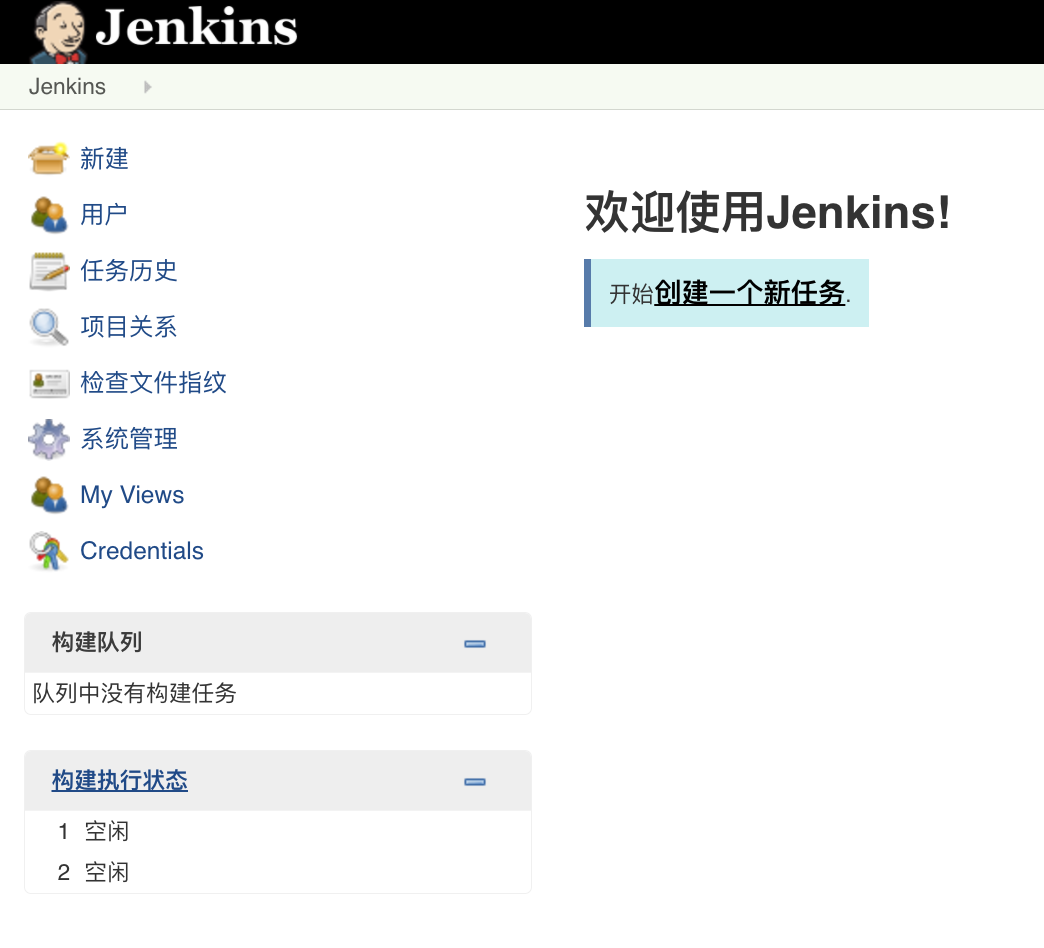
\includegraphics[width=5in]{chap02/jenkins3}
  \caption{Jenkins使用界面}
  \label{fig:jenkins3}
\end{figure}
% \begin{enumerate}
% \item 访问 http://mirrors.jenkins.io/war-stable/2.7.1/jenkins.war 下载2.7.1版本的jenkins安装包。
% \item 将jenkins.war 文件放到本地构建服务器(10.18.8.19)的Tomcat应用目录(/opt/tomcat/apache-tomcat-7.0.68/webapps)中。
% \item 配置并启动Tomcat即可完成安装,端口配置为8080,启动命令配置为:
% \begin{lstlisting}[language=bash,numbers=none]
% systemctl start/stop/status tomcat_jenkins.service
% \end{lstlisting}
% \item 访问jenkins地址(http://10.18.8.19:8080/jenkins/)初始化Jenkins:
% \begin{itemize}
% \item 完成认证,按照页面提示,将对应文件内容中的密码输入到文本框中,点击continue,如图\ref{fig:jenkins1}所示
% \begin{figure}[H] % use float package if you want it here
%   \centering
%   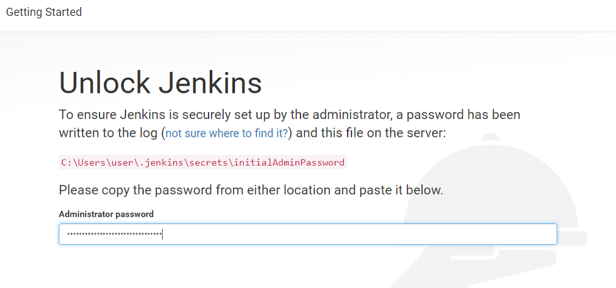
\includegraphics[width=5in]{chap02/jenkins1}
%   \caption{认证Jenkins界面}
%   \label{fig:jenkins1}
% \end{figure}
% \item 在插件选择处选择安装建议的插件
% \item 安装完成后在新的页面中配置用户名和密码完成安装,如图\ref{fig:jenkins2}
% \begin{figure}[H] % use float package if you want it here
%   \centering
%   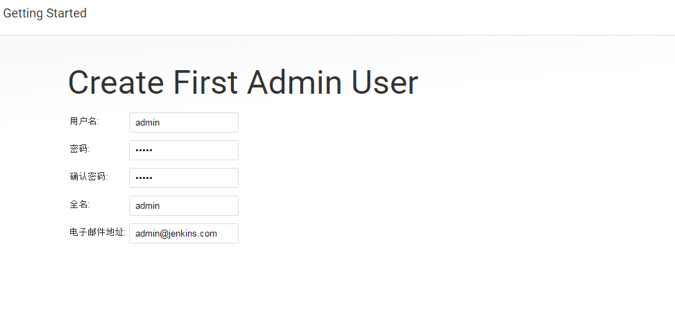
\includegraphics[width=5in]{chap02/jenkins2}
%   \caption{创建用户名和密码}
%   \label{fig:jenkins2}
% \end{figure}
% \item 进入图\ref{fig:jenkins3}页面表示安装成功
% \begin{figure}[H] % use float package if you want it here
%   \centering
%   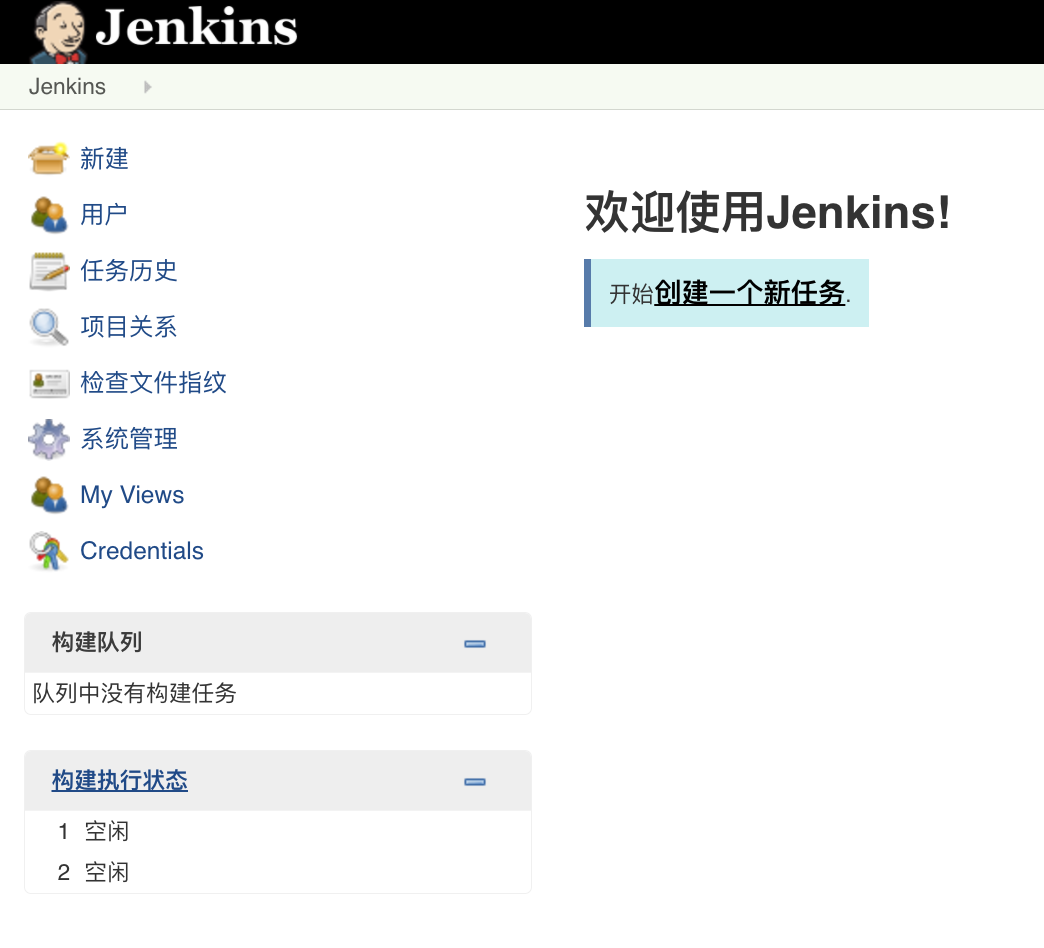
\includegraphics[width=5in]{chap02/jenkins3}
%   \caption{Jenkins使用界面}
%   \label{fig:jenkins3}
% \end{figure}
% \end{itemize}
% \end{enumerate}
\subsection{自动构建及检查方案设计}

由于小微平台通过Maven工具来解决代码使用过程中的函数依赖和本地项目构建\cite{董晓光2014使用},所以在进行自动构建的时候同样可以通过使用Maven Integration plugin插件实现项目的构建和代码检查,另外由于小微平台在开发过程中使用SVN来进行代码的版本控制,因此也需要在Jenkins中配置SVN插件来进行代码的同步和版本管理,除此之外,需要在安装Jenkins的服务器中提前安装好Maven软件。

小微项目在开发过程中通过前后端分离进行的开发,因此在构建过程中需要新建前端项目和后端项目,考虑到前端项目的构建相对后端项目比较简单,本论文只介绍后端项目的创建和构建过程。
\begin{itemize}
  \item 新建Jenkins项目
  \begin{enumerate}
    \item 在Jenkins主页面新建项目后,首先填写项目名称(以ServerDeployforPROD1.2为例)
    \item 源码管理配置为SVN,具体如图\ref{fig:jenkins4}所示:
      \begin{figure}[H] % use float package if you want it here
        \centering
        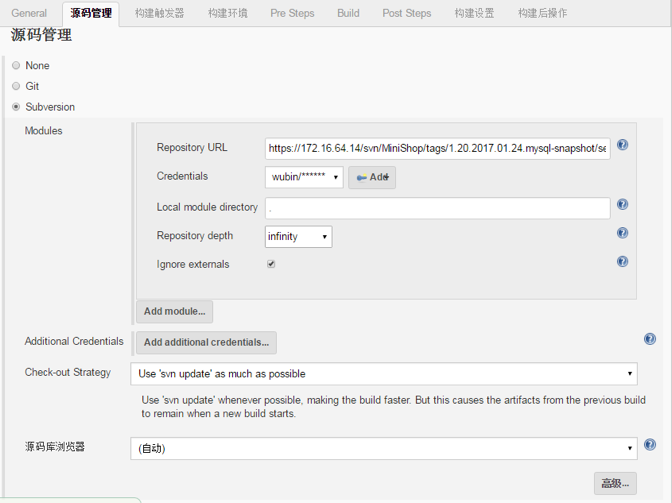
\includegraphics[width=6in]{chap02/jenkins4}
        \caption{Jenkins SVN配置}
        \label{fig:jenkins4}
      \end{figure}
      在对应的框中填写代码库的地址、通过Add按钮实现SVN的权限认证,其它选项选择默认即可。
    \item 在Pre Steps处增加shell命令为:
\begin{lstlisting}[language=bash,numbers=none]
rm -rf target/MiniShop
\end{lstlisting}
      确保每次构建时清除前一次构建信息。
    \item 在build标签页下配置构建时的操作,主要包括配置POM文件(pom.xml)的位置,pom.xml文件主要描述本Maven工程的整个生命周期所需要执行的功能和特性\cite{mileva2009mining},考虑到本项目的实际开发过程在这里选择项目pom2.xml
    \item 在Post Steps配置构建完成后的操作,首先需要在"Run only if build succeeds or is unstable"出打勾,保证在只有构建成功后才执行构建完成后的操作,其次需要配置构建完成对文件的操作:
\begin{lstlisting}[language=bash,numbers=none]
cp target/MiniShop.war /data/test/server/PROD/V1.2/MiniShop1.2_$(date +%Y%m%d)_$BUILD_NUMBER.war && chmod 777 /data/test/server/PROD/V1.2/MiniShop1.2_$(date +%Y%m%d)_$BUILD_NUMBER.war
\end{lstlisting}
      通过上述命令将每次构建完成后的文件进行备份保存和修改响应权限。
  \end{enumerate}
  所有项目信息配置完成后保存即可。
  \item 构建Jenkins项目

  进入项目主页,在页面左侧点击“立即构建”按钮即可进行构建,构建完成后将构建完成的war包上传到服务器即可,如果构建失败则表示在代码的书写过程中存在错误或者项目的库存在异常,需要在项目构建页面的构建信息页面中查看错误信息,并且根据错误信息来解决问题。
\end{itemize}

\subsection{自动部署方案设计}

Jenkins自动部署的方案是在每次构建完成后,让Jenkins可以自动的通过SSH协议访问远程服务器并将构建完成后的文件上传到服务器,并且执行服务器中的相应脚本来实现自动备份旧项目和部署新项目的目的。

\begin{enumerate}
  \item 在具体配置自动部署之前,需要先安装Publish Over SSH插件,通过这个插件,Jenkins可以实现通过SSH协议对远程服务器的访问。
  \item 在插件安装完成之后,需要配置插件来配置访问SSH的密钥和密码,在Jenkins“系统管理-系统设置”页面中会出现如图\ref{fig:jenkins5}配置:
    \begin{figure}[H] % use float package if you want it here
      \centering
      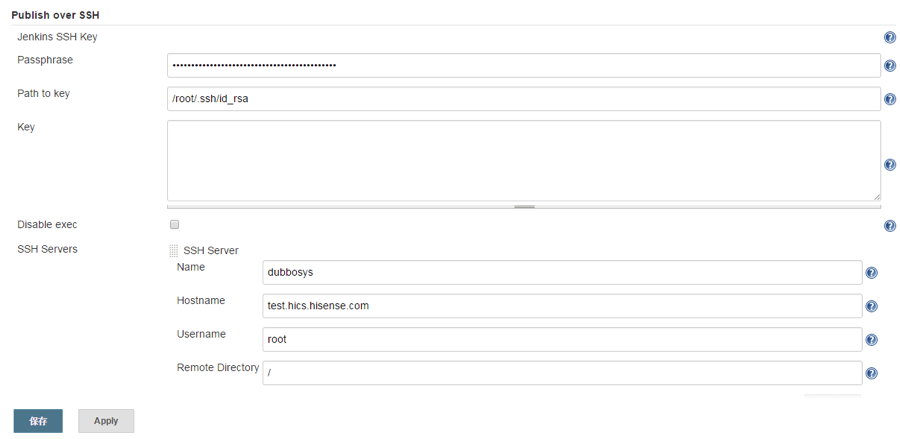
\includegraphics[width=6in]{chap02/jenkins5}
      \caption{Publish Over SSH插件配置}
      \label{fig:jenkins5}
    \end{figure}
  按照不同项目配置SSH Server信息和登录验证信息等。
  \item 插件配置完成后需要配置自动部署,插件安装完成后在“构建后操作”的选项中会出现“Send build artifacts over SSh”的选项,点击之后会出现配置:
    \begin{figure}[H] % use float package if you want it here
      \centering
      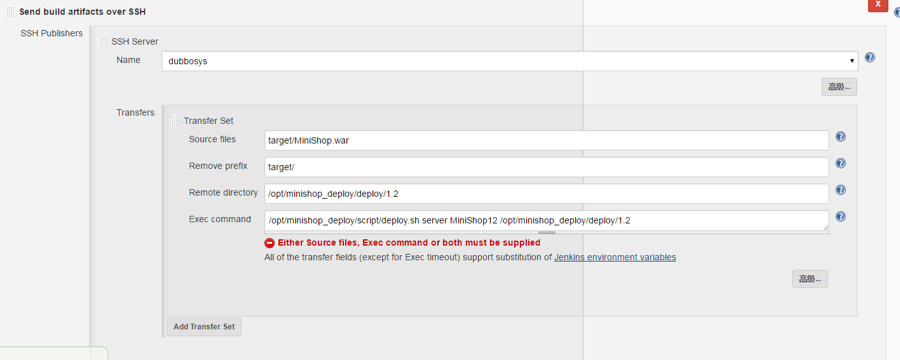
\includegraphics[width=7in]{chap02/jenkins6}
      \caption{Jenkins 自动部署配置}
      \label{fig:jenkins6}
    \end{figure}
  配置上传的文件名,上传后的路径,上传后需要执行的脚本和参数等,脚本可以参考附录\ref{cha:jenkinsdeploy}。
  \item 配置完成后再进行构建,Jenkins会自动的在构建后将构建生成的文件上传到服务器端指定路径,通过执行指定的脚本和参数将文件部署到Tomcat中,实现自动部署。
\end{enumerate}

\section{本章总结}

本章主要介绍了本人参与的小微项目的WEB平台所使用的开发框架、开发工具、开发过程以及系统上线的持续集成方案,通过持续集成方案增强了代码上线的稳定性,在本文后面的三章将会对本章开发的平台进行不通层级的优化,来实现本项目的安全性和高性能。
\chapter{应用性能优化}
\label{cha:ApplicationOptimization}
\section{Couchbase缓存优化}
目前大多数的WEB应用产品在设计开发的过程中对数据的读取还依旧通过直接对数据库进行增、删、改、查来实现。然而随着用户数量的增加,用户的请求也不断的增多,这对于数据库的压力是非常大的。之前的数据操作流程参见图~\ref{fig:couchbase1}。
\begin{figure}[H] % use float package if you want it here
  \centering
  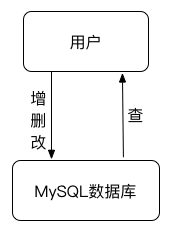
\includegraphics[width=1in]{chap03/couchbase1}
  \caption{通常数据操作流程}
  \label{fig:couchbase1}
\end{figure}
为了缓解数据库的压力,在数据的读取过程中将系统的基础数据读取到Couchbase缓存中,这样只需要对数据的基础数据进行一次读取即可完成数据的加载,降低了数据库的压力。通过缓存的数据操作流程参见图~\ref{fig:couchbase2}。
\begin{figure}[H] % use float package if you want it here
  \centering
  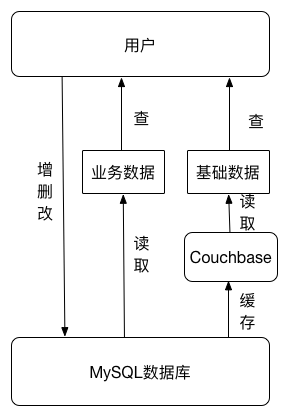
\includegraphics[width=1.7in]{chap03/couchbase2}
  \caption{通常数据操作流程}
  \label{fig:couchbase2}
\end{figure}
本论文中的WEB应用的数据包含基础数据和应用数据两部分,其中基础数据主要包括系统的基本配置数据、系统的常用变量数据、用户权限数据、枚举类型等相对固定的数据,这些数据在用户访问应用的时候只需要加载一次即可,不需要重复的从数据中读取,而应用数据则主要包含应用内的用户信息、商户信息、交易数据、库存数据等等不固定的数据,这些数据随着用户的时候会不断的发生变化,而且新的数据从数据库重新读取,这些数据在用户使用时需要多次加载。针对于以上不同数据的特点,将基础数据在用户首次登陆时加载到Couchbase缓存中,以后再读取时直接从缓存中读取。
\subsection{Couchbase安装}
\begin{enumerate}
\item 直接安装\cite{brown2012getting}

首先,通过浏览器访问\url{https://www.couchbase.com/nosql-databases/downloads}
,在页面中选择4.1.0版本、支持Red Hat 7平台的Couchbase Server安装文件couchbase-server-enterprise-4.1.0-centos7.x86\_64.rpm,将rpm文件复制到服务器中。或者直接在shell中通过
\begin{lstlisting}[language=bash,numbers=none]
$ wget https://packages.couchbase.com/releases/4.1.0/couchbase-server-enterprise-4.1.0-centos7.x86_64.rpm
\end{lstlisting}
命令将rpm安装文件下载到制定路径中。

然后,通过root用户访问Linux服务器,在终端中进入到couchbase安装文件所在路径,通过如下命令安装couchbase:
\begin{lstlisting}[language=bash,numbers=none]
$ rpm --install couchbase-server-enterprise-4.1.0-centos7.x86_64.rpm
\end{lstlisting}
安装完成后自动启动couchbase,并且会有如下提示信息:
\begin{lstlisting}[language=bash,numbers=none]
Warning: Transparent hugepages looks to be active and should not be.
Please look at http://bit.ly/1ZAcLjD as for how to PERMANENTLY alter this setting.
Minimum RAM required  : 4 GB
System RAM configured : 3.70 GB

Minimum number of processors required : 4 cores
Number of processors on the system    : 1 cores

Reloading systemd:                                         [  OK  ]
Starting couchbase-server (via systemctl):                 [  OK  ]

You have successfully installed Couchbase Server.
Please browse to http://iZ257vyhrvzZ:8091/ to configure your server.
Please refer to http://couchbase.com for additional resources.

Please note that you have to update your firewall configuration to
allow connections to the following ports: 11211, 11210, 11209, 4369,
8091, 8092, 8093, 9100 to 9105, 9998, 18091, 18092, 11214, 11215 and
from 21100 to 21299.

By using this software you agree to the End User License Agreement.
See /opt/couchbase/LICENSE.txt.
\end{lstlisting}
couchbase默认安装位置为“/opt/couchbase/”

\item Docker安装\cite{merkel2014docker}

\begin{lstlisting}[language=bash,numbers=none]
# 下载镜像
$ docker pull couchbase:4.1.0
# 运行容器
$ docker run -d --name db -p 8091-8094:8091-8094 -p 11210:11210 couchbase
\end{lstlisting}

\end{enumerate}
Couchbase安装完成后,需要在阿里云的安全策略中配置外网访问的端口和应用访问的端口,相关配置参见\ref{cha:Monitor-aliyun}
\subsection{Couchbase集群配置}
Couchbase服务器及可以单独运行,也可以将多个服务器组成一个集群,作为集群来运行。通过Couchbase集群,可以实现缓存数据的分布式存储及负载均衡,提升缓存的高可用以及系统的性能。

Couchbase数据分布是按计算分配到多个节点上,每个节点都储存两部分数据有效数据和副本数据,客户端对数据的操作主要是按照节点中对应的有效数据进行操作,执行压力会部分到不同的节点,如~\ref{fig:couchbase3}所示:
\begin{figure}[H] % use float package if you want it here
  \centering
  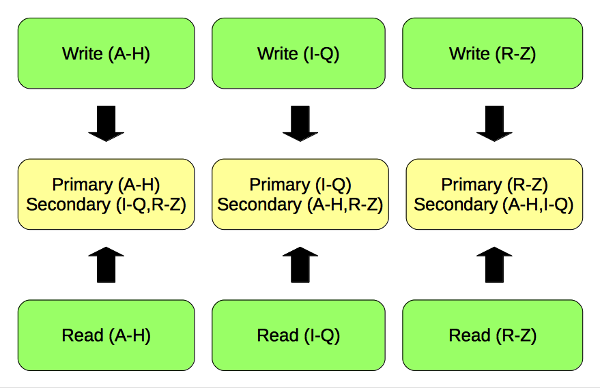
\includegraphics[width=3in]{chap03/couchbase3}
  \caption{Couchbase集群数据操作模型}
  \label{fig:couchbase3}
\end{figure}
Couchbase的集群管理是由erlang/otp进行集群通信管理,集群之间使用心跳机制进行监测服务器节点健康监测,配置参数信息是同步到每一个节点上进行储存。整个集群以vbucket为单位划分映射到不同服务器节点中进行储存,划分规则如下:
\begin{enumerate}
\item 均匀的分配有效vbucket和副本vbucket到不同服务器节点中;
\item 把有效数据与副本数据划分到不同物理节点中;
\item 在复制多份数据时,尽量有其它节点进行数据传播;
\item 扩展时,以最小化数据迁移量进行复制。
\end{enumerate}

在Couchbase负载均衡中,我们所操作的每一个bucket会逻辑划分为1024个vbucket,其数据的储存基于每个vbucket储存并且每个 vbucket都会映射到相对应的服务器节点,这种储存结构的方式叫做集群映射。如~\ref{fig:couchbase4}所示,当应用与Couchbase服务器交互时,会通过SDK的与 服务器数据进行交互,当应用操作某一个的bucket的key值时,在SDK中会通过哈希的方式计算,使用公式crc32(key)%1024确定key 值是属于1024个vbucket中的某个,然后根据vbucket所映射的节点服务器对数据进行操作。
\begin{figure}[H] % use float package if you want it here
  \centering
  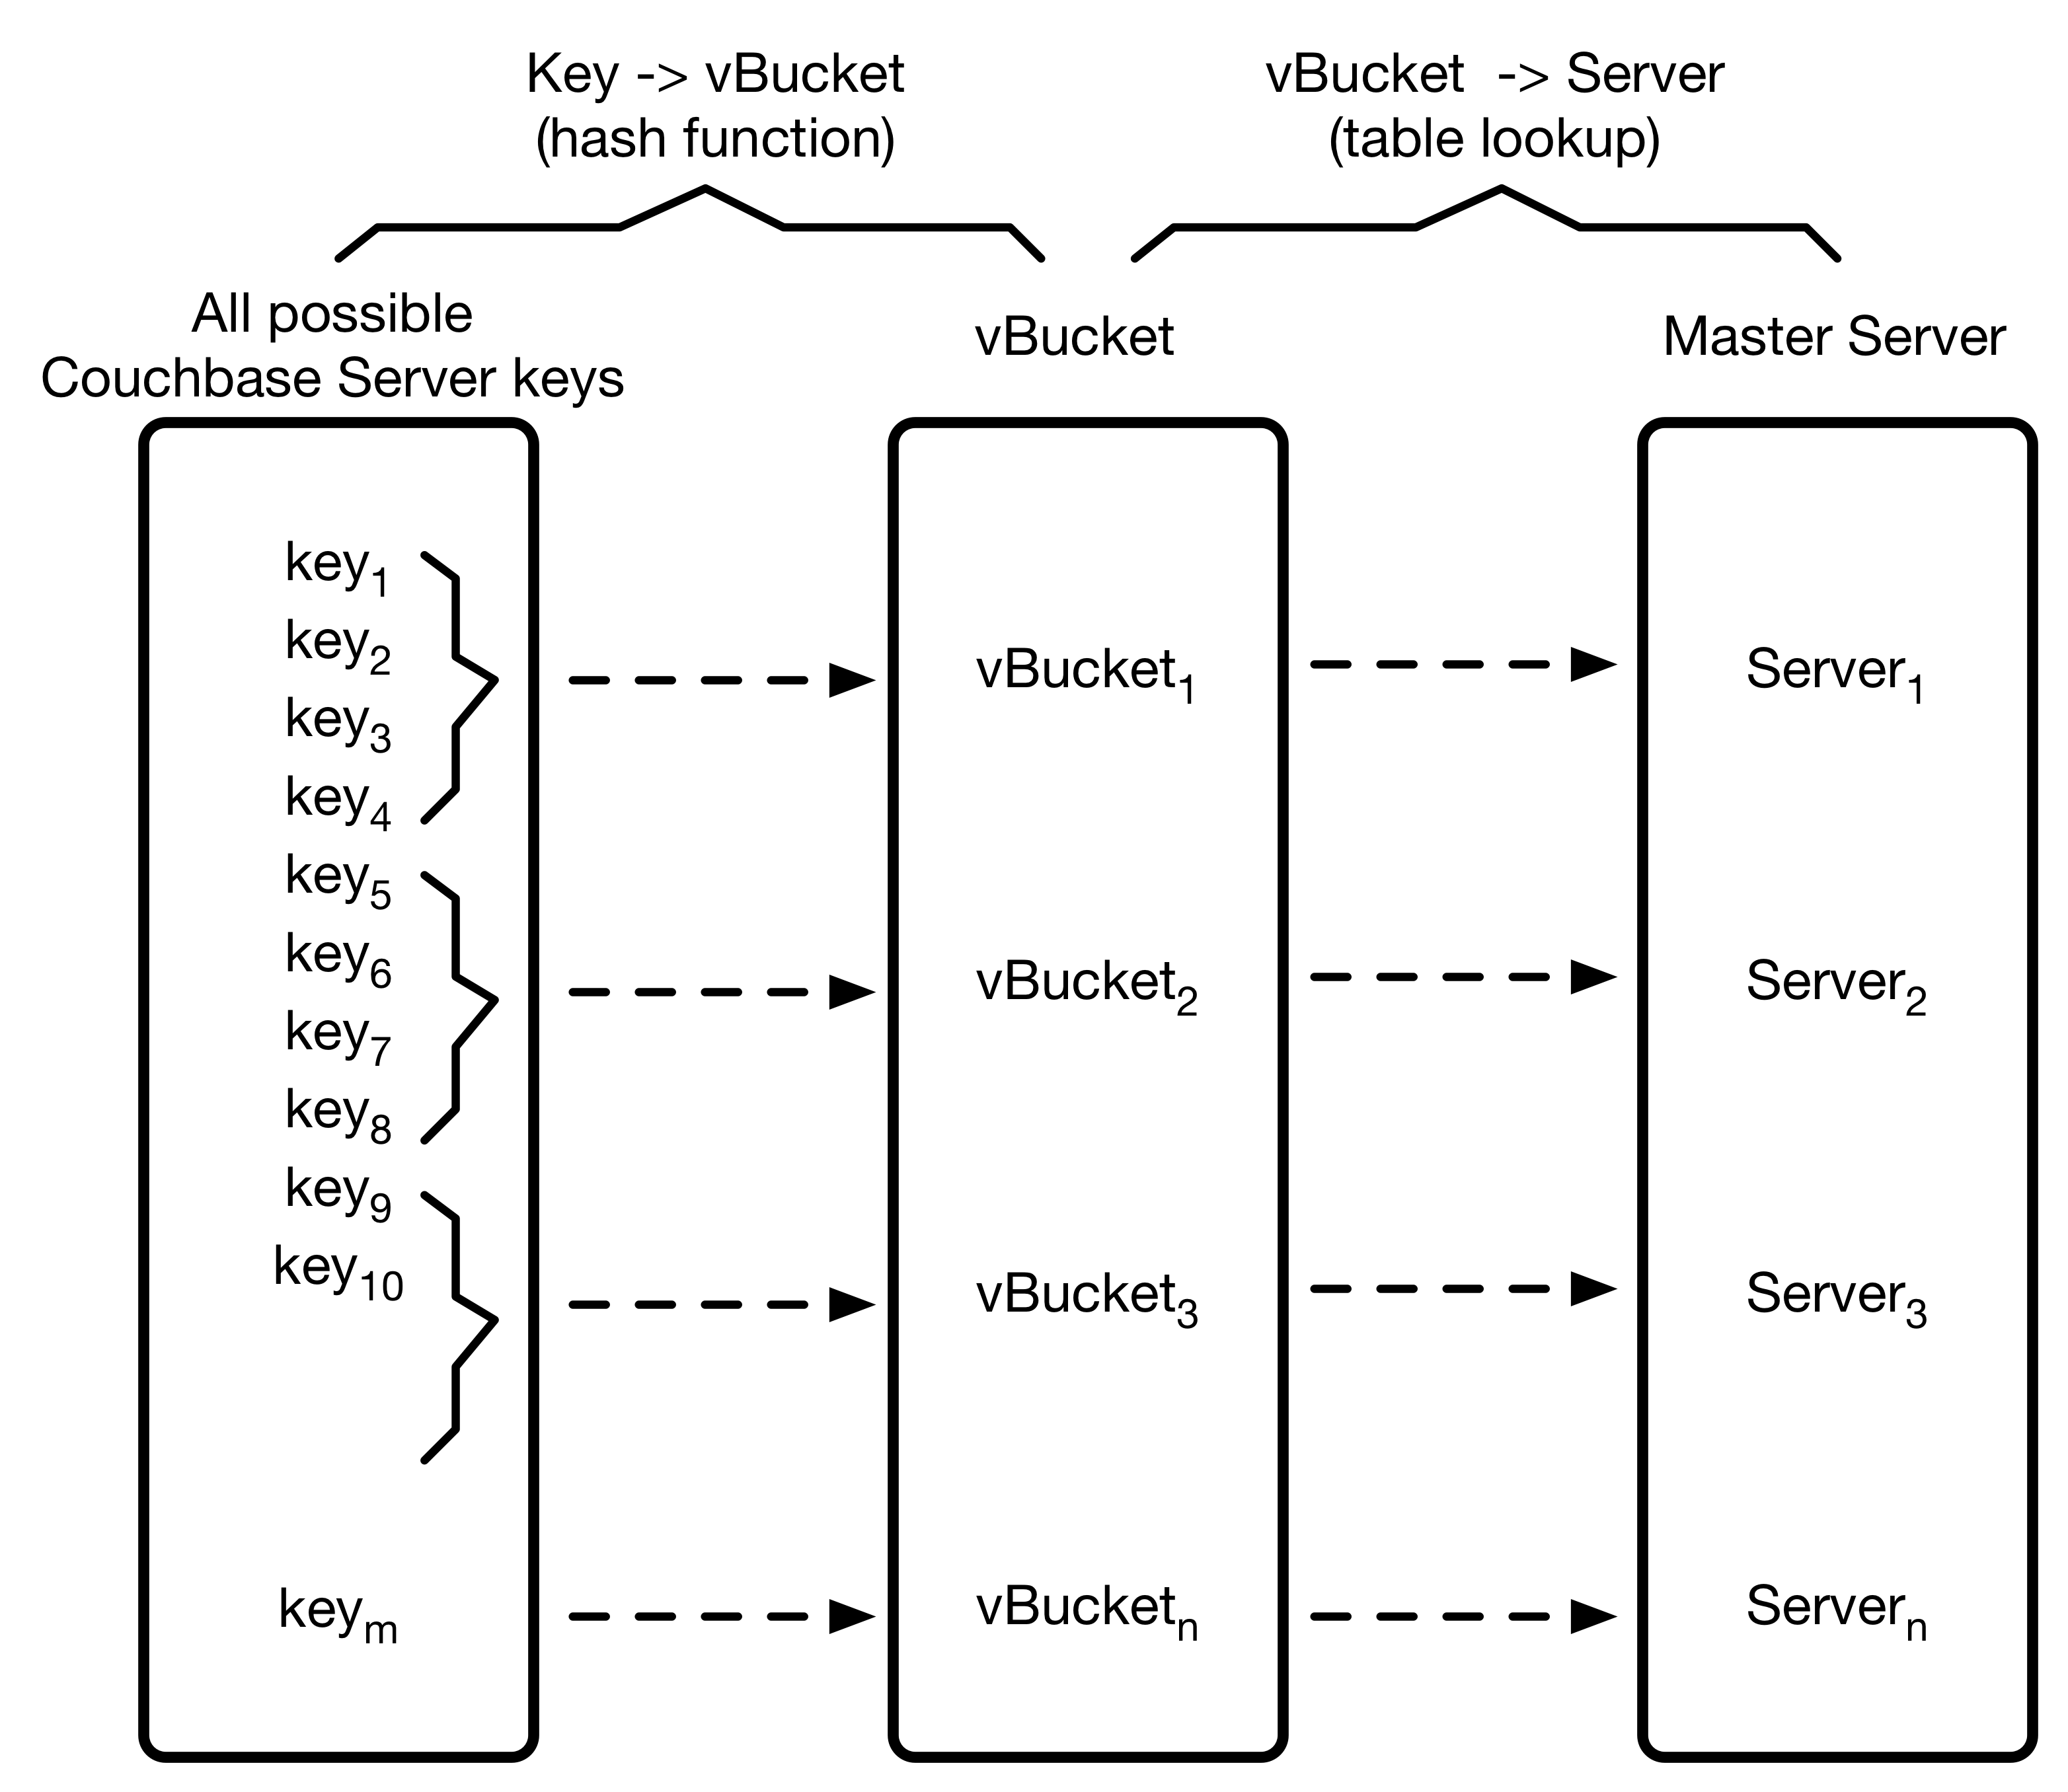
\includegraphics[width=3in]{chap03/couchbase4}
  \caption{Couchbase负载均衡模型}
  \label{fig:couchbase4}
\end{figure}
在设置标签页中的集群标签页下新建和配置集群信息
\begin{figure}[H] % use float package if you want it here
  \centering
  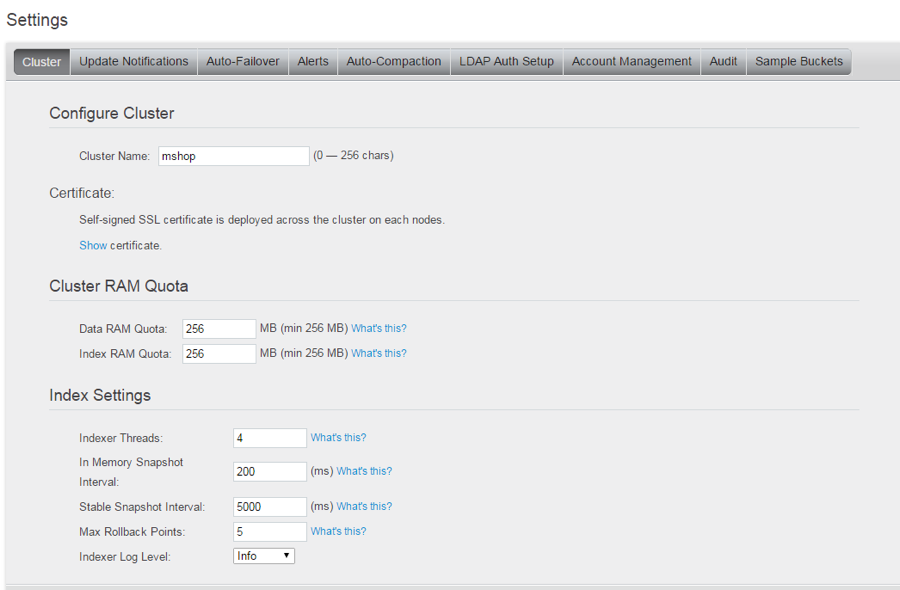
\includegraphics[width=3in]{chap03/couchbase5}
  \caption{Couchbase创建集群}
  \label{fig:couchbase5}
\end{figure}
在服务器节点标签页下新增服务器节点
\begin{figure}[H] % use float package if you want it here
  \centering
  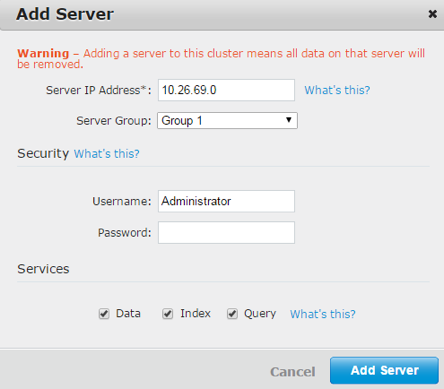
\includegraphics[width=3in]{chap03/couchbase6}
  \caption{Couchbase增加节点}
  \label{fig:couchbase6}
\end{figure}
增加完服务器节点后可以看到集群的基本信息
\begin{figure}[H] % use float package if you want it here
  \centering
  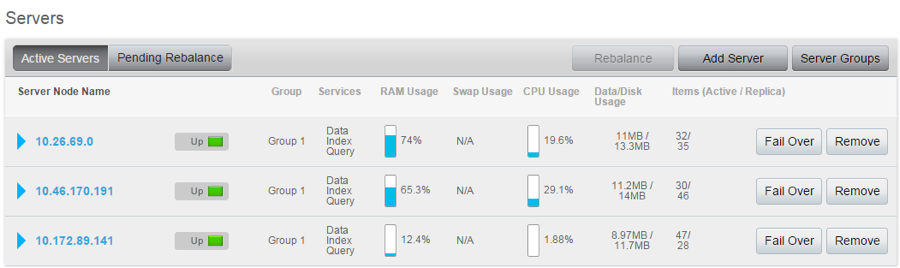
\includegraphics[width=3in]{chap03/couchbase7}
  \caption{Couchbase集群概览}
  \label{fig:couchbase7}
\end{figure}

% \subsection{Couchbase数据存取配置}
% \begin{enumerate}
% \item 启用couchbase
% 在项目的配置文件中增加config-couchbase的配置文件,并增加配置文件如下:
% \begin{lstlisting}[language=Java4]
% couchBase.maxWait=6000
% couchBase.maxclientPoolSize=2
% couchBase.minClientPoolSize=2
% couchBase.clientIncrease=1
% couchBase.bucketName=default
% couchBase.server=localhost:8091
% couchBase.serverPwd=
% # if use couchbase
% couchBase.inUsed=1
% \end{lstlisting}
% 在spring.xml文件中增加Couchbase的链接项和配置项。
% \item 数据存储

% \item 数据更新
% \end{enumerate}
\subsection{Couchbase缓存对系统性能影响}
通过ab命令对使用应用进行压力测试,在开启couchbase和关闭couchbase的情况下分别模拟5万个请求,每次并发10个请求来对比缓存对系统性能的影响:
\begin{lstlisting} [language=bash]
$ ab -n 50000 -c 10 -k http://test.hics.hisense.com:8081/client/mnsindex.html
This is ApacheBench, Version 2.3 <$Revision: 1748469 $>
Copyright 1996 Adam Twiss, Zeus Technology Ltd, http://www.zeustech.net/
Licensed to The Apache Software Foundation, http://www.apache.org/

Benchmarking test.hics.hisense.com (be patient)
Completed 5000 requests
Completed 10000 requests
Completed 15000 requests
Completed 20000 requests
Completed 25000 requests
Completed 30000 requests
Completed 35000 requests
Completed 40000 requests
Completed 45000 requests
Completed 50000 requests
Finished 50000 requests


Server Software:        nginx/1.9.12
Server Hostname:        test.hics.hisense.com
Server Port:            8081

Document Path:          /client/mnsindex.html
Document Length:        36028 bytes

Concurrency Level:      10
Time taken for tests:   206.318 seconds
Complete requests:      50000
Failed requests:        0
Keep-Alive requests:    49504
Total transferred:      1816897520 bytes
HTML transferred:       1801400000 bytes
Requests per second:    242.34 [#/sec] (mean)
Time per request:       41.264 [ms] (mean)
Time per request:       4.126 [ms] (mean, across all concurrent requests)
Transfer rate:          8599.92 [Kbytes/sec] received

Connection Times (ms)
              min  mean[+/-sd] median   max
Connect:        0    0   0.1      0       5
Processing:    20   41  19.1     38    1146
Waiting:       16   31   8.9     30    1058
Total:         20   41  19.2     38    1147

Percentage of the requests served within a certain time (ms)
  50%     38
  66%     44
  75%     47
  80%     49
  90%     54
  95%     62
  98%     75
  99%     86
 100%   1147 (longest request)
\end{lstlisting}
\begin{lstlisting} [language=bash]
$ ab -n 50000 -c 10 -k http://test.hics.hisense.com/client/mnsindex.html
This is ApacheBench, Version 2.3 <$Revision: 1748469 $>
Copyright 1996 Adam Twiss, Zeus Technology Ltd, http://www.zeustech.net/
Licensed to The Apache Software Foundation, http://www.apache.org/

Benchmarking test.hics.hisense.com (be patient)
Completed 5000 requests
Completed 10000 requests
Completed 15000 requests
Completed 20000 requests
Completed 25000 requests
Completed 30000 requests
Completed 35000 requests
Completed 40000 requests
Completed 45000 requests
Completed 50000 requests
Finished 50000 requests


Server Software:        Apache-Coyote/1.1
Server Hostname:        test.hics.hisense.com
Server Port:            80

Document Path:          /client/mnsindex.html
Document Length:        36028 bytes

Concurrency Level:      10
Time taken for tests:   247.137 seconds
Complete requests:      50000
Failed requests:        0
Keep-Alive requests:    49505
Total transferred:      1814097525 bytes
HTML transferred:       1801400000 bytes
Requests per second:    202.32 [#/sec] (mean)
Time per request:       49.427 [ms] (mean)
Time per request:       4.943 [ms] (mean, across all concurrent requests)
Transfer rate:          7168.40 [Kbytes/sec] received

Connection Times (ms)
              min  mean[+/-sd] median   max
Connect:        0    0   0.1      0      12
Processing:    21   49  17.5     45     528
Waiting:       17   27  12.0     24     504
Total:         21   49  17.6     45     528

Percentage of the requests served within a certain time (ms)
  50%     45
  66%     49
  75%     51
  80%     53
  90%     63
  95%     69
  98%     88
  99%    104
 100%    528 (longest request)
\end{lstlisting}
\section{Tomcat高并发APR优化}
Tomcat对用户请求的处理方式有BIO、NIO以及APR三种方式,其中BIO模式为Tomcat的默认处理方式\cite{vukotic2011securing}。

BIO模式是一种阻塞式I/O操作,这种模式表示Tomcat使用的是传统Java I/O操作。在这种模式下对于每个请求都要创建一个线程来处理,线程开销较大,不能处理高并发的场景,在三种模式中性能也最低。启动tomcat看到如图~\ref{fig:tomcat1}所示日志,表示使用的是BIO模式:
\begin{figure}[H] % use float package if you want it here
  \centering
  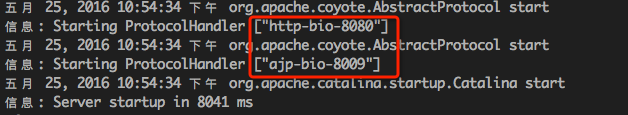
\includegraphics[width=3in]{chap03/tomcat1}
  \caption{BIO模式日志}
  \label{fig:tomcat1}
\end{figure}
NIO模式是Java SE 1.4及后续版本提供的一种新的I/O操作方式。该模式是一个基于缓冲区、并能提供非阻塞I/O操作的Java API,它拥有比传统I/O操作(bio)更好的并发运行性能。启动tomcat看到如图~\ref{fig:tomcat2}所示日志,表示使用的是NIO模式:
\begin{figure}[H] % use float package if you want it here
  \centering
  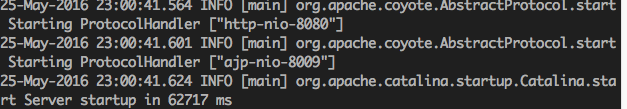
\includegraphics[width=3in]{chap03/tomcat2}
  \caption{NIO模式日志}
  \label{fig:tomcat2}
\end{figure}
APR模式是从操作系统级别解决异步IO问题,大幅度的提高服务器的处理和响应性能, 也是Tomcat运行高并发应用的首选模式。启动tomcat看到如图~\ref{fig:tomcat3}所示日志,表示使用的是NIO模式:
\begin{figure}[H] % use float package if you want it here
  \centering
  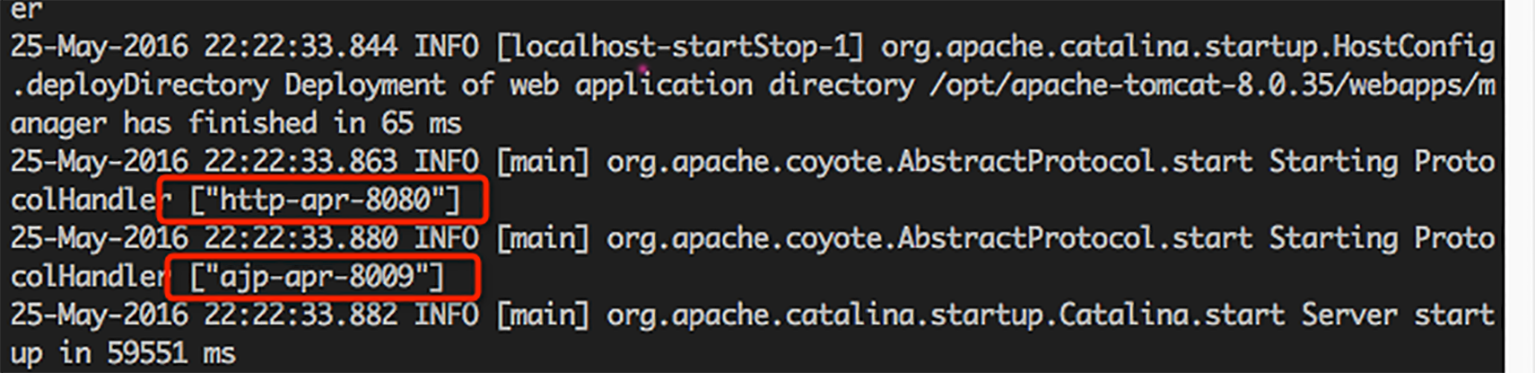
\includegraphics[width=3in]{chap03/tomcat3}
  \caption{APR模式日志}
  \label{fig:tomcat3}
\end{figure}
考虑到应用在大量用户访问的情况下必然会出现高并发的现象,因此调整Tomcat的请求处理方式为APR模式对于提升系统的高并发处理能力时非常必要的\cite{蒋文旭2012大型高并发}。

APR(Apache Portable Runtime)是一个高可移植库,它是Apache HTTP Server 2.x的核心。APR有很多用途,包括访问高级IO功能(例如sendfile,epoll和OpenSSL),OS级别功能(随机数生成,系统状态等等),本地进程管理(共享内存,NT管道和UNIX sockets)。这些功能可以使Tomcat作为一个通常的前台WEB服务器,能更好地和其它本地web技术集成,总体上让Java更有效率作为一个高性能web服务器平台而不是简单作为后台容器。

在产品环境中,特别是直接使用Tomcat做WEB服务器的时候,应该使用Tomcat Native来提高其性能,要测APR给tomcat带来的好处最好的方法是在慢速网络上(模拟Internet),将Tomcat线程数开到300以上的水平,然后模拟一大堆并发请求。

如果不配APR,基本上300个线程狠快就会用满,以后的请求就只好等待。但是配上APR之后,并发的线程数量明显下降,从原来的300可能会马上下降到只有几十,新的请求会毫无阻塞的进来。
在局域网环境测,就算是400个并发,也是一瞬间就处理/传输完毕,但是在真实的Internet环境下,页面处理时间只占0.1\%都不到,绝大部分时间都用来页面传输。如果不用APR,一个线程同一时间只能处理一个用户,势必会造成阻塞。所以生产环境下用apr是非常必要的。
\subsection{开启APR模式}

\subsection{APR模式对于系统性能的影响}
\section{Docker分布式优化}
随着用户数量的增加以及应用业务的扩展,目前WEB应用的数据库服务器已经由一台服务器扩展为两台服务器,应用服务器也已经由一台服务器扩展为两台服务器,加上目前的测试服务器,一共有5台服务器服务于一个WEB应用,而且在未来的发展过程中,无论是数据节点还是应用节点,数量肯定时不断增加的。在节点不断增加的情况下,如何快速部署一个数据库节点或者一个应用节点必然是运维人员在新增节点时必须要面对的问题。

在新增节点上部署服务的方式主要有直接安装以及容器技术两种方式,其中直接安装的方式依靠手动的在服务器中安装各种库以及依赖,然后安装应用软件病进行配置,这种方式在快速部署一个节点的过程中的劣势非常明显。

目前实现快速部署新增节点的解决方案主要有虚拟机技术和容器技术两种技术,其中传统虚拟机技术是虚拟出一套硬件后,在其上运行一个完整操作系统,在该系统上再运行所需应用进程,如图~\ref{fig:docker1}所示;而容器内的应用进程直接运行于宿主的内核,容器内没有自己的内核,而且也没有进行硬件虚拟。因此容器要比传统虚拟机更为轻便如图~\ref{fig:docker2}所示\cite{刘熙2016基于}。

\begin{figure}[H] % use float package if you want it here
  \centering
  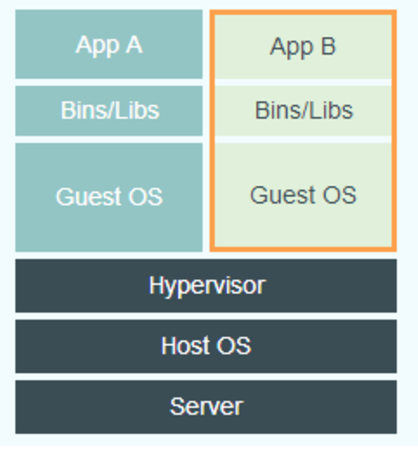
\includegraphics[width=3in]{chap03/docker1}
  \caption{传统虚拟机模型}
  \label{fig:docker1}
\end{figure}
\begin{figure}[H] % use float package if you want it here
  \centering
  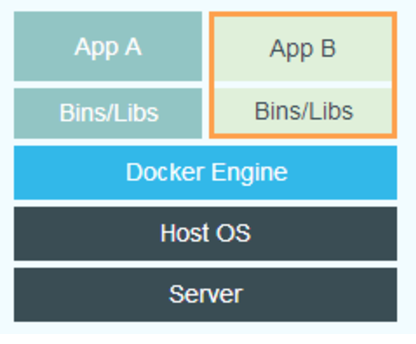
\includegraphics[width=3in]{chap03/docker2}
  \caption{Docker容器模型}
  \label{fig:docker2}
\end{figure}
同传统的虚拟机技术相比,Docker容积技术具有非常多的优势,这也是本论文中使用Docker技术作为WEB应用开发过程中服务器扩展的主要技术。
\begin{itemize}
\item 更高效的利用系统资源

由于容器不需要进行硬件虚拟以及运行完整操作系统等额外开销,Docker 对系统资源的利用率更高。无论是应用执行速度、内存损耗或者文件存储速度,都要比传统虚拟机技术更高效。因此,相比虚拟机技术,一个相同配置的主机,往往可以运行更多数量的应用。
\item 更快速的启动时间

传统的虚拟机技术启动应用服务往往需要数分钟,而 Docker 容器应用,由于直接运行于宿主内核,无需启动完整的操作系统,因此可以做到秒级、甚至毫秒级的启动时间。大大的节约了开发、测试、部署的时间。
\item 一致的运行环境

开发过程中一个常见的问题是环境一致性问题。由于开发环境、测试环境、生产环境不一致,导致有些 bug 并未在开发过程中被发现。而 Docker 的镜像提供了除内核外完整的运行时环境,确保了应用运行环境一致性,从而不会再出现 “这段代码在我机器上没问题啊” 这类问题。
\item 持续交付和部署

对开发和运维(DevOps)人员来说,最希望的就是一次创建或配置,可以在任意地方正常运行。

使用 Docker 可以通过定制应用镜像来实现持续集成、持续交付、部署。开发人员可以通过 Dockerfile 来进行镜像构建,并结合 持续集成(Continuous Integration) 系统进行集成测试,而运维人员则可以直接在生产环境中快速部署该镜像,甚至结合 持续部署(Continuous Delivery/Deployment) 系统进行自动部署。

而且使用 Dockerfile 使镜像构建透明化,不仅仅开发团队可以理解应用运行环境,也方便运维团队理解应用运行所需条件,帮助更好的生产环境中部署该镜像。
\item 更轻松的迁移

由于 Docker 确保了执行环境的一致性,使得应用的迁移更加容易。Docker 可以在很多平台上运行,无论是物理机、虚拟机、公有云、私有云,甚至是笔记本,其运行结果是一致的。因此用户可以很轻易的将在一个平台上运行的应用,迁移到另一个平台上,而不用担心运行环境的变化导致应用无法正常运行的情况。
\item 更轻松的维护和扩展

Docker 使用的分层存储以及镜像的技术,使得应用重复部分的复用更为容易,也使得应用的维护更新更加简单,基于基础镜像进一步扩展镜像也变得非常简单。此外,Docker 团队同各个开源项目团队一起维护了一大批高质量的官方镜像,既可以直接在生产环境使用,又可以作为基础进一步定制,大大的降低了应用服务的镜像制作成本。
\item 对比传统虚拟机总结
\begin{table}[H]
  \centering
  \begin{minipage}[t]{0.8\linewidth} % 如果想在表格中使用脚注,minipage是个不错的办法
  % \caption[模板文件]{模板文件。如果表格的标题很长,那么在表格索引中就会很不美
  %   观,所以要像 chapter 那样在前面用中括号写一个简短的标题。这个标题会出现在索
  %   引中。}
  \label{tab:docker-compare}
    \begin{tabularx}{\linewidth}{lXX|}
      \toprule[1.5pt]
      {\heiti 对比参数} & {\heiti 容器技术} & {\heiti 虚拟机技术}\\\midrule[1pt]
      启动时间  &  秒级 & 分钟级 \\
      硬盘使用  &  一般为MB  &  一般为GB\\
      应用性能  &  接近原生  &  弱于\\
      系统支持量 & 单机支持上千个容器 & 一般几十个\\
      \bottomrule[1.5pt]
    \end{tabularx}
  \end{minipage}
\end{table}
\end{itemize}

\subsection{使用Docker Compose管理Docker容器}
在Docker安装完成后,可以通过docker pull 命令下载相应的镜像,通过ducker run运行镜像,生成一个运行中的容器。除了通过ducker run命令运行容器以外,还可以通过Docker Compose工具来快速在集群中部署分布式应用以及容器的管理工作。

使用Docker Compose 项目是 Docker 官方的开源项目,负责实现对 Docker 容器集群的快速编排。它的定位是 “定义和运行多个 Docker 容器的应用(Defining and running multi-container Docker applications),它允许用户通过一个单独的 docker-compose.yml 模板文件(YAML 格式)来定义一组相关联的应用容器为一个项目(project)。

Compose 中有两个重要的概念:
\begin{itemize}
\item 服务(service):一个应用的容器,实际上可以包括若干运行相同镜像的容器实例。
\item 项目(project):由一组关联的应用容器组成的一个完整业务单元,在 docker-compose.yml 文件中定义。
\end{itemize}
Compose 的默认管理对象是项目,通过子命令对项目中的一组容器进行便捷地生命周期管理。

Compose 项目由 Python 编写,实现上调用了 Docker 服务提供的 API 来对容器进行管理。因此,只要所操作的平台支持 Docker API,就可以在其上利用 Compose 来进行编排管理。

对于Mysql可以通过修改docker-compose.yml文件来实现数据库镜像的运行以及容器的相关控制:
\begin{lstlisting} [language=sh,numbers=none]
version: '2'
services:
    mysql_master:
        image: docker.io/mysql
        restart: always
        container_name: mysql-master
        ports:
            - "3306:3306"
        volumes:
            - ./master/conf:/etc/mysql/conf.d
            - ./master/data:/var/lib/mysql
            - /etc/localtime:/etc/localtime:ro
        environment:
            MYSQL_ROOT_PASSWORD: "*********"
    mysql_slave:
        image: docker.io/mysql
        restart: always
        container_name: mysql-slave
        ports:
            - "3307:3306"
        volumes:
            - ./slave/conf:/etc/mysql/conf.d
            - ./slvae/data:/var/lib/mysql
            - /etc/localtime:/etc/localtime:ro
        environment:
            MYSQL_ROOT_PASSWORD: "*********"
\end{lstlisting}
上述配置文件通过运行docker.io/mysql镜像生成两个mysql容器,其中一个的端口为3306,另一个的端口为3307,这样能够很方面的创建两个容器。同样,根据这个方法也可以创建多个相互关联的容器,比如Tomcat和Mysql的相互关联。
\subsection{应用容器化现状}
根据现阶段的项目开发和服务器运维需求,已经在生产环境的两个数据库服务器中通过Docker实现了Mysql数据库容器的运行,在生产环境的两个应用服务器中实现了Couchbase应用的容器化,在测试环境的服务器中实现了测试环境数据库、测试环境Couchbase、生产环境服务器Couchbase节点、生产环境延时备份数据库的容器化。这样,当部署一个新的服务器节点的时候,可以通过Docker容器快速部署数据库应用、Couchbase应用。

目前考虑到Tomcat在运行过程中需要面临频繁修改的配置文件、库文件以及其他工具的配置等问题,Docker Hub中官方的Tomcat镜像无法满足项目开发的实际需求,暂时没有实现Tomat的容器化。为了后期Tomcat的容器化,目前也正在预研通过Dockerfile定制镜像的方式定制符合项目需求的Tomcat镜像,预研工作完成后即进行Tomcat的容器话需求。

由于Docker Hub的官方镜像服务器在国外,在本地服务器中通过docker pull 命令下载镜像的速度太慢,难以满足快速部署的需求,故在生产环境的一个服务器节点中部署了本地的Docker 镜像源,后期在新节点可以通过docker pull本地的镜像源来下载官方的以及定制的docker镜像。
\section{SLB负载均衡优化}

随着用户访问的增加以及服务高可用的需求,单个应用节点无法满足项目的需求,因此需要通过增加应用服务器节点来实现WEB应用的高可用,并且通过负载均衡将用户的请求转发到不同的服务器,降低单个服务器节点的压力。

负载均衡(Load balancing)是一种计算机网络技术,用来在多个计算机(计算机集群)、网络连接、CPU、磁盘驱动器或其他资源中分配负载,以达到最佳化资源使用、最大化吞吐率、最小化响应时间、同时避免过载的目的。

使用带有负载均衡的多个服务器组件,取代单一的组件,可以通过冗余提高可靠性。

负载平衡最重要的一个应用是利用多台服务器提供单一服务,这种方案有时也称之为服务器农场。通常,负载平衡主要应用于Web网站,大型的Internet Relay Chat网络,高流量的文件下载网站,NNTP(Network News Transfer Protocol)服务和DNS服务。现在负载平衡器也开始支持数据库服务,称之为数据库负载平衡器。
对于互联网服务,负载平衡器通常是一个软体程序,这个程序侦听一个外部端口,互联网用户可以通过这个端口来访问服务,而作为负载平衡器的软体会将用户的请求转发给后台内网服务器,内网服务器将请求的响应返回给负载平衡器,负载平衡器再将响应发送到用户,这样就向互联网用户隐藏了内网结构,阻止了用户直接访问后台(内网)服务器,使得服务器更加安全,可以阻止对核心网络栈和运行在其它端口服务的攻击。
当所有后台服务器出现故障时,有些负载平衡器会提供一些特殊的功能来处理这种情况。例如转发请求到一个备用的负载平衡器、显示一条关于服务中断的消息等。负载平衡器使得IT团队可以显著提高容错能力。它可以自动提供大量的容量以处理任何应用程序流量的增加或减少\cite{wei2010system}。

负载均衡的主要特点有:
\begin{enumerate}
\item 解决并发压力,提高应用处理性能(增加吞吐量,加强网络处理能力);
\item 提供故障转移,实现高可用;
\item 通过添加或减少服务器数量,提供网站伸缩性(扩展性);
\item 安全防护;(负载均衡设备上做一些过滤,黑白名单等处理);
\end{enumerate}

考虑到本项目中的所有服务器节点均为阿里云云服务器,故选择通过使用阿里云的负载均衡服务器服务(SLB)来进行应用的负载均衡,通过创建一个负载均衡服务,即可获取到一个公网的IP,通过配置监听,将WEB应用的http协议端口(80)和https(443)协议分别转发到生产环境各应用服务器节点的Tomcat对应端口,通过配置服务器节点的权重来决定负载均衡在转发用户请求时向后端服务器转发的比重。

\section{本章总结}
本章主要是对WEB应用的应用性能进行优化,主要包括通过配置Couchbase缓存机制,将应用的基础数据加载到缓存中,在提升应用的相应速度的同时降低了数据库的压力;通过调整Tomcat的请求处理方式为APR模式,提升Tomcat对于高并发的处理能力;通过Docker容器编排技术将应用通过容器的方式运行在服务器中,实现了节点快速部署应用的能力;通过配置应用负载均衡,在提升服务的高可用性的同时降低了服务器节点的压力。

\chapter{数据优化}
\label{cha:Database}
在WEB应用的开发和使用过程中,数据对于应用的价值越来越重要,因此在应用的使用过程中,保证数据库的正常工作以及数据的完整性将成为开发过程中数据库优化的主要目标。

目前应用开发过程中使用的数据库是MySQL,MySQL是一个开源的关系数据库管理系统,通过关系模型为用户提供数据的存储和修改等操作。

最新的稳定版为5.7.17,项目所使用的MySQL版本为5.7.11。较之前的版本,5.7版本的主要改进包括以下几个方面:
\begin{enumerate}
    \item 提升安全性

    为了增强数据库数据的安全性,在完成MySQL安装时,默认的root密码不再为空,而是随机生成一个密码,用户可以通过随机密码登录MySQL后修改密码。除此之外,新版本删除了test数据库,并且对用户创建的test数据库的权限进行了控制,同时提供了更为简单SSL安全访问配置,对于用户的密码可以设置有效期策略,超过有效期时强制用户修改密码来保证数据库的安全,新版本还新增了对用户的暂时禁用功能。
    \item 增强数据存储的灵活性

    新版本在提升数据存储的灵活性方面增加了JSON和generate column两个新功能。

    随着非结构化数据存储需求的持续增长,各种非结构化数据存储的数据库应运而生(如MongoDB)。从最新的数据库使用排行榜来看,MongoDB已经超过了PostgreSQL,其火热程度可见一斑。各大关系型数据库也不甘示弱,纷纷提供对JSON的支持,以应对非结构化数据库的挑战。MySQL数据库从5.7.8版本开始,也提供了对JSON的支持。使用方式如下:
\begin{lstlisting}[numbers=none]
CREATE TABLE t1 (jdoc JSON);
INSERT INTO t1 VALUES('{"key1": "value1", "key2": "value2"}');
\end{lstlisting}
MySQL对支持JSON的做法是,在server层提供了一堆便于操作JSON的函数,至于存储,就是简单地将JSON编码成BLOB,然后交由存储引擎层进行处理,也就是说,MySQL 5.7的JSON支持与存储引擎没有关系,MyISAM 存储引擎也支持JSON 格式。

MySQL支持JSON以后,总是避免不了拿来与MongoDB进行比较。但是,MySQL对JSON的支持,至少有两点能够完胜MongoDB:
\begin{enumerate}
\item 可以混合存储结构化数据和非结构化数据,同时拥有关系型数据库和非关系型数据库的优点
\item 能够提供完整的事务支持
\end{enumerate}

generated column是MySQL 5.7引入的新特性,所谓generated column,就是数据库中这一列由其他列计算而得。
\item 提升数据库运行的易用性

在开发或者运维人员进行数据库使用和状态检查的过程中,MySQL 5.7可以explain一个正在运行的SQL,这对于DBA分析运行时间较长的语句将会非常有用,同时performance\_schema提供了更多监控信息,包括内存使用,MDL锁,存储过程等。

除此之外,MySQL 5.7.7中引入了一个系统库sys schema,它包含了一系列视图、函数和存储过程, 该项目专注于MySQL的易用性。例如,我们可以通过sys schema快速的知道,哪些语句使用了临时表,哪个用户请求了最多的io,哪个线程占用了最多的内存,哪些索引是无用索引等

sys schema中包含了大量的视图,视图中的信息均来自performance schema统计信息。也就是说,performance schema提供了信息源,但是没有很好的将这些信息组织成有用的信息,从而没有很好的发挥它们的作用。而sys schema使用performance schema信息,通过视图的方式给出解决实际问题的答案。

例如,下面这些问题,在MySQL 5.7之前,需要借助外部工具才能知道,在MySQL 5.7中,直接查询sys库下相应的表就能得到答案:
\begin{lstlisting}[language=sql,numbers=none]
# 如何查看数据库中的冗余索引
select * from sys.schema_redundant_indexes;
# 如何获取未使用的索引
select * from schema_unused_indexes;
# 如何查看使用全表扫描的SQL语句
select * from statements_with_full_table_scans
\end{lstlisting}
\item 提升了数据库的可用性

在以往的版本中,许多数据库的设置修改都需要重启服务使配置生效,在5.7版本中增加了许多改进,可以使一些必要的配置无需重启服务即可生效。

在线设置复制的过滤规则不再需要重启MySQL,只需要停止SQL thread,修改完成以后,启动SQL thread。

在线开启GTID,在之前的版本中,由于不支持在线开启GTID,用户如果希望将低版本的数据库升级到支持GTID的数据库版本,需要先关闭数据库,再以GTID模式启动,所以导致升级起来很繁琐。MySQL 5.7以后,这个问题得到了妥善的解决。

在线修改buffer pool的大小,MySQL 5.7为了支持online buffer pool resize,引入chunk的概念,每个chunk默认是128M,当我们在线修改buffer pool的时候,以chunk为单位进行增长或收缩。这个参数的引入,对innodb\_buffer\_pool\_size的配置有了一定的影响。innodb要求buffer pool size是innodb\_buffer\_pool\_chunk\_size* innodb\_buffer\_pool\_instances的倍数,如果不是,将会适当调大innodb\_buffer\_pool\_size以满足要求,因此,可能会出现buffer pool的实际分配比配置文件中指定的size要大的情况.

Online DDL MySQL 5.7支持重命名索引和修改varchar的大小,这两项操作在之前的版本中,都需要重建索引或表.
\begin{lstlisting}[language=sql,numbers=none]
ALTER TABLE t1 ALGORITHM=INPLACE, CHANGE COLUMN c1 c1 VARCHAR(255);
\end{lstlisting}

\item 性能相关的改进
\begin{itemize}
\item 只读事务性能改进

众所周知,在传统的OLTP应用中,读操作远多于写操作,并且,读操作不会对数据库进行修改,如果是非锁定读,读操作也不需要进行加锁。因此,对只读事务进行优化,是一个不错的选择。

MySQL 5.6中,已经对只读事务进行了许多优化。例如,将MySQL内部实现中的事务链表分为只读事务链表和普通事务链表,这样在创建ReadView的时候,需要遍历事务链表的长度就会小很多。

在MySQL 5.7中,首先假设一个事务是一个只读事务,只有在该事务发起了修改操作时,才会将其转换为一个普通事务。MySQL 5.7通过避免为只读事务分配事务ID,不为只读事务分配回滚段,减少锁竞争等多种方式,优化了只读事务的开销,提高了数据库的整体性能。
\item 加速连接处理

在MySQL 5.7之前,变量的初始化操作(THD、VIO)都是在连接接收线程里面完成的,现在将这些工作下发给工作线程,以减少连接接收线程的工作量,提高连接的处理速度。这个优化对那些频繁建立短连接的应用,将会非常有用。
\item 复制性能的改进

MySQL的复制延迟是一直被诟病的问题之一,欣喜的是,MySQL 5.7版本已经支持"真正"的并行复制功能。MySQL 5.7并行复制的思想简单易懂,简而言之,就是”一个组提交的事务都是可以并行回放的”,因为这些事务都已进入到事务的prepare阶段,则说明事务之间没有任何冲突(否则就不可能提交)。 经过对比测试,MySQL 5.7采用新的并行复制后,仍然会存在一定程度的延迟,只不过相比5.6版本减少了86\%,相比MariaDB的并行复制延迟也小不少。复制延迟问题得到极大改善。

除此之外复制性能的改进还包括多源复制,多从线程增强,在线 GTIDs和增强的半同步复制等功能,这些功能均为保证数据的完整性和有效性提高了保障。
\end{itemize}
\end{enumerate}

在数据库开发过程中,存储引擎对于数据库性能也非常重要,它是我们在进行数据的存储、数据索引的建立、数据的更新以及数据查询的内部实现方法~\cite{胡雯2012mysql}。

同MySQL数据库相比,Oracle 数据库和 SQL Server数据库只使用一种数据库引擎,所有的数据操作方法都是采用一种方法。MySQL 数据库为了改变这种局面,为用户提供了多种引擎,开发者在开发过程中可以根据应用的自身需求为数据配置更加合适的数据库引擎。MySQL数据库提供的存储引擎如表~\ref{tab:mysql-engine}所示。

\begin{table}[H]
  \centering
  \begin{minipage}[t]{0.8\linewidth} % 如果想在表格中使用脚注,minipage是个不错的办法
  \caption[MySQL]{MySQL数据库存储引擎}
  \label{tab:mysql-engine}
    \begin{tabularx}{\linewidth}{lX}
      \toprule[1.5pt]
      {\heiti 存储引擎} & {\heiti 描述}\\\midrule[1pt]
      InnoDB  &  支持事务和行级锁,是Mysql上唯一一个提供了外键约束的引擎  \\
      MyISAM  &  基于ISAM存储引擎,常用的引擎,但是不支持事务、行级锁、而且崩溃后不能保证完全恢复。  \\
      ARCHIVE  &  仅支持插入和查询以及索引功能,拥有很好的压缩机制,适用于存储日志信息或其他按时间序列实现的数据采集类的应用场景中  \\
      CSV & 将数据文件保存为CSV格式的的文件,可以方便的导入到其他数据库中去,但是不支持索引 \\
      BLACKHOLE & 没有存储机制,任何数据都会被丢弃,但是会记录二进制日志\\
      FEDERATED & 可以访问远程服务器上数据的存储引擎,所以说它不再本地创建数据只会自动的建立一个连接到其他服务器上链接,有点类似于代理的功能\\
      MEMORY & 使用存储在内存中的内存来创建表,而且所有数据保存在内存中,数据安全性很低,但是查找和插入速度很快,通常用于临时表\\
      MRG\_MYISAM & 将多个MyISAM合并为一个\\
      \bottomrule[1.5pt]
    \end{tabularx}
  \end{minipage}
\end{table}

这些数据引擎中使用最广泛的是 MyISAM 和 InnoDB 两种存储引擎。前者是MySQL数据库的默认存储引擎,后者则是第三方公司开发的,它跟前者相比,后者具有支持事务、支持行级锁以及支持外键约束等非常实用的功能~\cite{胡雯2012mysql}。

% \begin{enumerate}
% \item 支持事务安全。InnoDB存储引擎最重要的一点就是对事务安全的支持,这也是让它成为最流行的存储引擎很重要的原因,而且实现了SQL92标准所定义的4个级别(READ UNCOMMITTED, READ COMMITTED, REPEATABLE READ, SERIALIZABLE)\cite{胡雯2012mysql}.
% \item 数据库多版本读取。InnoDB在事务支持的同时,为了保证数据的一致性以及并发时刻的性能,通过对un-do信息的聚簇索引实现对数据的多版本读取。
% \item 锁定机制的改进。InnoDB改变了MyISAM的锁机制,实现了行锁。虽然InnoDB的行锁机制是通过索引来完成的,但是由于数据库中99\%的 SQL 语句都是通过索引来检索数据,所以行锁机制为InnoDB在承受高并发下的环境下增强了竞争力。
% \item 实现外键。InnoDB实现了外键引用这一数据库的重要特性,使得在数据库端控制部分数据的完整性成为可能。
% \end{enumerate}

\section{InnoDB引擎参数优化}

设计InnoDB引擎的目的是解决MySQL在处理非常大的数据量时表现出性能不足的问题。通过使用InnoDB引擎,对于服务器的CPU运行效率来说性能远远超过了其它关系型数据库引擎,因此在开发数据量比较大的应用时,InnoDB引擎已经受到了很多开发者的认可。~\cite{schwartz2012high}。由于InnoDB数据引擎在事务安全、支持外键以及数据恢复成本的综合性能表现,本论文中的WEB应用数据存储引擎使用的是InnoDB引擎。

为了保证在使用InnoDB引擎过程中,使WEB应用的数据稳定性和服务器负载达到最优,还需要基于目前的WEB开发架构和服务器现状对MySQL的配置进行一定的参数调优。优化主要包括内存、IO、日志以及其它方面\cite{顾治华2006mysql}。

\begin{enumerate}
\item 内存利用方面

在内存利用方面,innodb\_buffer\_pool\_*相关的参数主要负载调控数据库在运行过程中数据缓存到内存的数据。其中innodb\_buffer\_pool\_size是InnoDB最重要的一个配置参数,也是在进行Innodb引擎优化时第一个需要调整的参数,它的主要作用是对Innodb的索引进行缓存。参数的默认分配只有8M,如果在配置过程中不调整这个值的话,会导致数据库的性能体验过差。

除此之外,还可以通过调整innodb\_buffer\_pool\_instances 来修改数据库缓冲池的实例数量,通过开启多个内存缓冲池,把需要缓冲的数据hash到不同的缓冲池中,这样可以进行并行的内存读写,在高IO负载时保持非常稳定的吞吐。

一般来说pool size参数和pool instance参数之前相互配置,通过不断的测试来调优二者的值,最终使数据库的内存利用方面达到最高。
\item IO控制方面

对于数据库的空间占用,可以通过修改innodb\_file\_*参数来配置,考虑到阿里云的磁盘扩展和读取的性能,这个参数的配置对于数据库的性能提升效果不明显,因此没有必要做配置。

对于数据的IO分配来说,需要进行一定的优化,可以通过innodb\_file\_format配置文件的格式,提升存储数据的压缩比,可以通过修改innodb\_thread\_concurrency参数来配置线程的并发数,提升效率。
\item 日志控制方面

通过修改innodb\_log\_file\_size参数可以调整每个日志文件的大小,每个日志文件的大小对于服务器磁盘的写入和异常恢复后的恢复效率有非常大的影响,因此需要合理配置该参数值,由于当前的数据库服务器是阿里云数据库,硬盘为高速硬盘,数据的存取效率和IO压力均表现良好,故这个参数对于当前项目来说没有优化的必要。

通过修改innodb\_log\_buffer\_size参数可以日志缓冲区的大小,这个值分配的大小与内存中缓存的日志大小有很大的关系,适当修改这个值可以降低内存的压力。

除了正常的日志外,InnoDB还有undo log,它记录某数据被修改前的值,可以用来在事务失败时进行回滚,因此通过调整undo log的相关参数可以在很大程度上保证数据的有效性。通过修改innodb\_undo\_log\_truncate参数值为1来开启在线回收undo 日志文件,通过修改innodb\_max\_undo\_log\_size参数值来配置触发回收undo 日志的阈值,通过innodb\_purge\_rseg\_truncate\_frequency参数来配置回收undo 日志的频率~\cite{fruhwirt2010innodb}。
\item 其它方面优化

除了以上三个方面的优化之外,还有许多优化项目可以应用于本项目的数据库优化中。考虑到阿里云磁盘的性能,可以通过innodb\_flush\_method参数将数据和日志文件不经过缓存直接写入到文件中;通过innodb\_strict\_mode参数开启严格模式,对于写法错误的SQL语句跳过警告直接提示错误,提升数据库的稳定性;通过脏页的相关配置参数调整数据库对于脏页的刷新方式和效率,提升数据的有效性。
\end{enumerate}
综合以上各个方面的优化之后,本论文中WEB应用的数据库InnoDB引擎优化参数如表~\ref{tab:mysql-innodb}所示:
\begin{longtable}[hc]{{l}{c}{l}}
\caption{InnoDB优化参数}\label{tab:mysql-innodb}\\
\toprule[1.5pt]
{\heiti 参数项} & {\heiti 参数内容}  & {\heiti 参数描述} \\\midrule[1pt]
\endfirsthead
\multicolumn{3}{c}{续表~\thetable\hskip1em InnoDB优化参数}\\
\toprule[1.5pt]
{\heiti 参数项} & {\heiti 参数内容}  & {\heiti 参数描述} \\\midrule[1pt]
\endhead
\hline
\multicolumn{3}{r}{续下页}
\endfoot
\endlastfoot
      innodb\_buffer\_pool\_size  & 800M &  缓冲池字节大小\\
      innodb\_buffer\_pool\_instances  & 8 &  缓冲池实例数量 \\
      innodb\_buffer\_pool\_load\_at\_startup  & 1 & 启动时将热数据加载到内存 \\
      innodb\_buffer\_pool\_dump\_at\_shutdown & 1 &  关闭时将热数据dump到本地磁盘\\
      innodb\_lru\_scan\_depth & 2000 & page cleaner线程每次刷新脏页的数量\\
      innodb\_lock\_wait\_timeout & 5 & 事务等待获取资源等待的最长时间\\
      innodb\_io\_capacity & 4000 & 调整刷新脏页的数量\\
      innodb\_io\_capacity\_max & 8000 & 刷新脏页的最大值\\
      innodb\_flush\_method & O\_DIRECT & 数据和日志写入磁盘的方式-直接写入磁盘\\
      innodb\_file\_format & Barracuda & 文件格式,Barracuda支持压缩页,新格式 \\
      innodb\_file\_format\_max & Barracuda &  设置文件格式最高版本\\
      innodb\_flush\_neighbors & 1 & 刷新脏页临近页  \\
      innodb\_log\_buffer\_size & 1M & 用来缓冲日志数据的缓冲区大小   \\
      innodb\_purge\_threads & 4 &  单独的清除线程数量  \\
      innodb\_large\_prefix  & 1 & 为字段创建索引时限制的字节长度,超过直接报错    \\
      innodb\_thread\_concurrency  & 64 &  线程并发数  \\
      innodb\_print\_all\_deadlocks & 1 &  将发生的所有死锁信息都记录到错误日志中  \\
      innodb\_strict\_mode & 1 &  严格检查模式,写法有错误直接报错,不警告  \\
      innodb\_sort\_buffer\_size & 10485760 &  建立索引时用于排序数据的排序缓冲区大小-10M  \\
      innodb\_buffer\_pool\_dump\_pct & 40 &  转储缓冲池中的最近使用的页的占比  \\
      innodb\_page\_cleaners & 4 &  page cleaner线程数量  \\
      innodb\_undo\_log\_truncate & 1 &  开启在线回收undo log日志文件  \\
      innodb\_max\_undo\_log\_size & 2G &  超过这个阈值时触发回收 \\
      innodb\_purge\_rseg\_truncate\_frequency & 128 &  回收undo日志的频率  \\
\bottomrule[1.5pt]
\end{longtable}


\section{主从复制和延迟复制优化}

除了通过InnoDB引擎的配置来保证数据的有效性和稳定性之外,在数据库的开发和使用过程中还可以通过配置主从复制和延迟复制来保证数据的完整性。在5.7以前的MySQL版本中,由于主从复制的延迟问题,通常会选择第三方工具来进行数据的同步,但是通过第三方工具,对于数据同步的稳定性又带来了问题,这些问题一直是运维人员在数据库开发过程中比较头疼的问题。随着5.7版本的发布,新版本在数据库主从复制方面进行了很多改进,包括降低了复制的延迟,通过looseless半同步方式提升了复制的稳定性\cite{朱振2013基于}。

MySQL数据库复制技术是把数据从一个数据库节点拷贝到其它一个或者多个数据库节点中,前者通常被称为主库(Master),后者通常被称为从库(Slave),如图\ref{fig:replication1}所示。
\begin{figure}[H] % use float package if you want it here
  \centering
  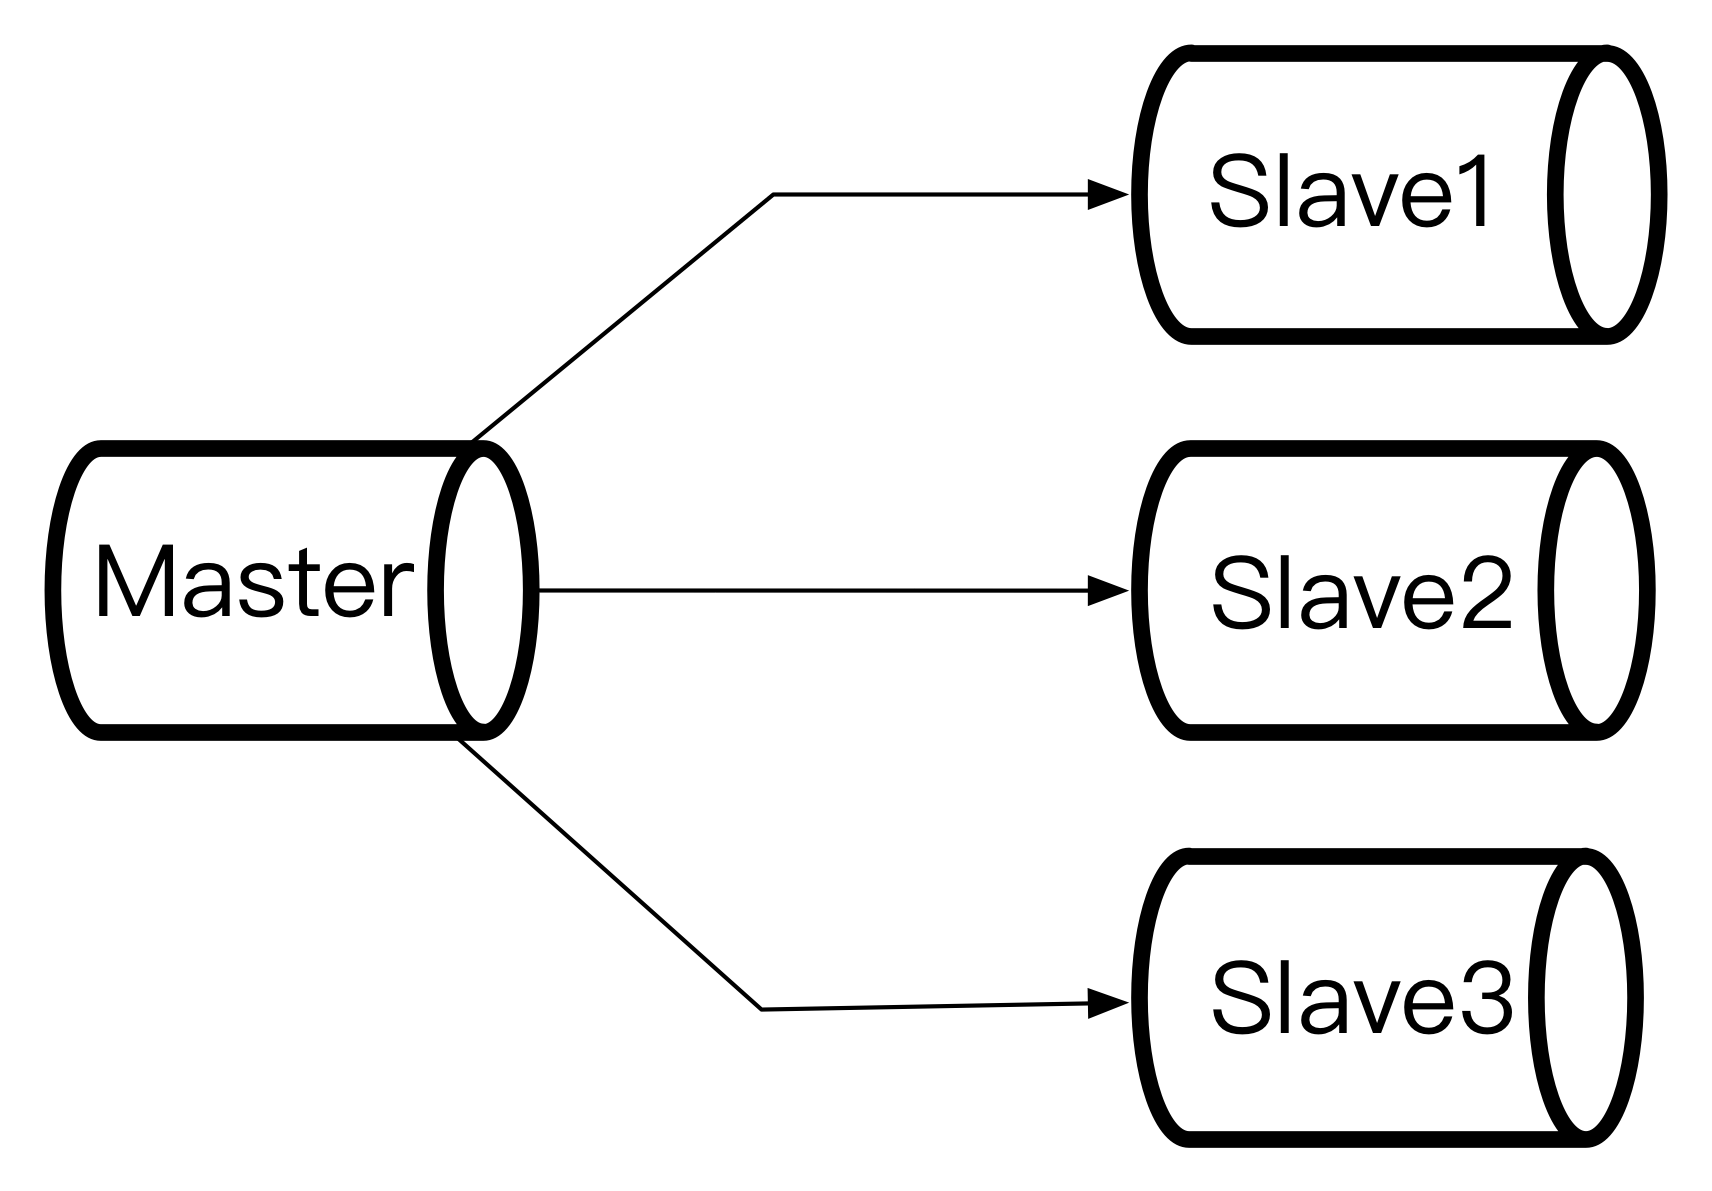
\includegraphics[width=3in]{chap04/replication1}
  \caption{MySQL复制示意图}
  \label{fig:replication1}
\end{figure}

复制的结果是集群(Cluster)中的所有数据库服务器得到的数据理论上都是一样的,都是同一份数据,只是有多个copy。MySQL默认内建的复制策略是异步的,基于不同的配置可以调整复制策略,Slave不一定要一直和Master保持连接不断的复制或等待复制,我们可以指定复制所有的数据库,一部分数据库或者是某个数据库的某部分表。

MySQL复制支持多种不同的复制策略,包括同步、半同步、异步和延迟策略等。
\begin{enumerate}
\item 同步策略:Master要等待所有Slave应答之后才会提交(MySql对DB操作的提交通常是先对操作事件进行二进制日志文件写入然后再进行提交)。
\item 半同步策略:Master等待至少一个Slave应答就可以提交。
\item 异步策略:Master不需要等待Slave应答就可以提交。
\item 延迟策略:Slave要至少落后Master指定的时间。
\end{enumerate}
MySQL复制同时支持多种不同的复制模式:
\begin{enumerate}
\item 基于语句的复制Statement Based Replication(SBR)。
\item 基于行的复制Row Based Replication(RBR)。
\item 混合复制(Mixed)。
\end{enumerate}
使用MySQL复制,对于系统性能的提升主要表现在以下几个方面:
\begin{enumerate}
\item 性能方面:MySQL复制是一种Scale-out方案,也即“水平扩展”,将原来的单点负载扩散到多台Slave机器中去,从而提高总体的服务性能。在这种方式下,所有的写操作,当然包括UPDATE操作,都要发生在Master服务器上。读操作发生在一台或者多台Slave机器上。这种模型可以在一定程度上提高总体的服务性能,Master服务器专注于写和更新操作,Slave服务器专注于读操作,我们同时可以通过增加Slave服务器的数量来提高读服务的性能。

\item 防腐化:由于数据被复制到了Slave,Slave可以暂停复制进程,进行数据备份,因此可以防止数据腐化。

\item 故障恢复:同时多台Slave如果有一台Slave挂掉之后我们还可以从其他Slave读取,如果配置了主从切换的话,当Master挂掉之后我们还可以选择一台Slave作为Master继续提供写服务,这大大增加了应用的可靠性。

\item 数据分析:实时数据可以存储在Master,而数据分析可以从Slave读取,这样不会影响Master的性能。
\end{enumerate}
\subsection{数据库复制流程}
MySQL复制最常用的复制方式是通过二进制文件的方式进行复制,因此在配置数据库复制时,需要在主服务器和从服务器中开启二进制日志的配置。

数据库的复制过程主要可以分为三步:
\begin{enumerate}
\item 当主数据库的数据发生改变时,主数据库会将数据库数据记录的事务过程写到已经开启的二进制日志文件中;
\item 主库将事务写入二进制文件后会通知从库数据,此时从数据库会链接主数据库将改变的事务日志下载到从数据库的中继日志中;
\item 从数据库对于中继日志中的新事务进行重放,根据日志操作方式修改从数据库的对应数据,保证数据的一致\cite{秦金2013分布式}。
\end{enumerate}
图~\ref{fig:replication2}描述了复制的过程
\begin{figure}[H] % use float package if you want it here
  \centering
  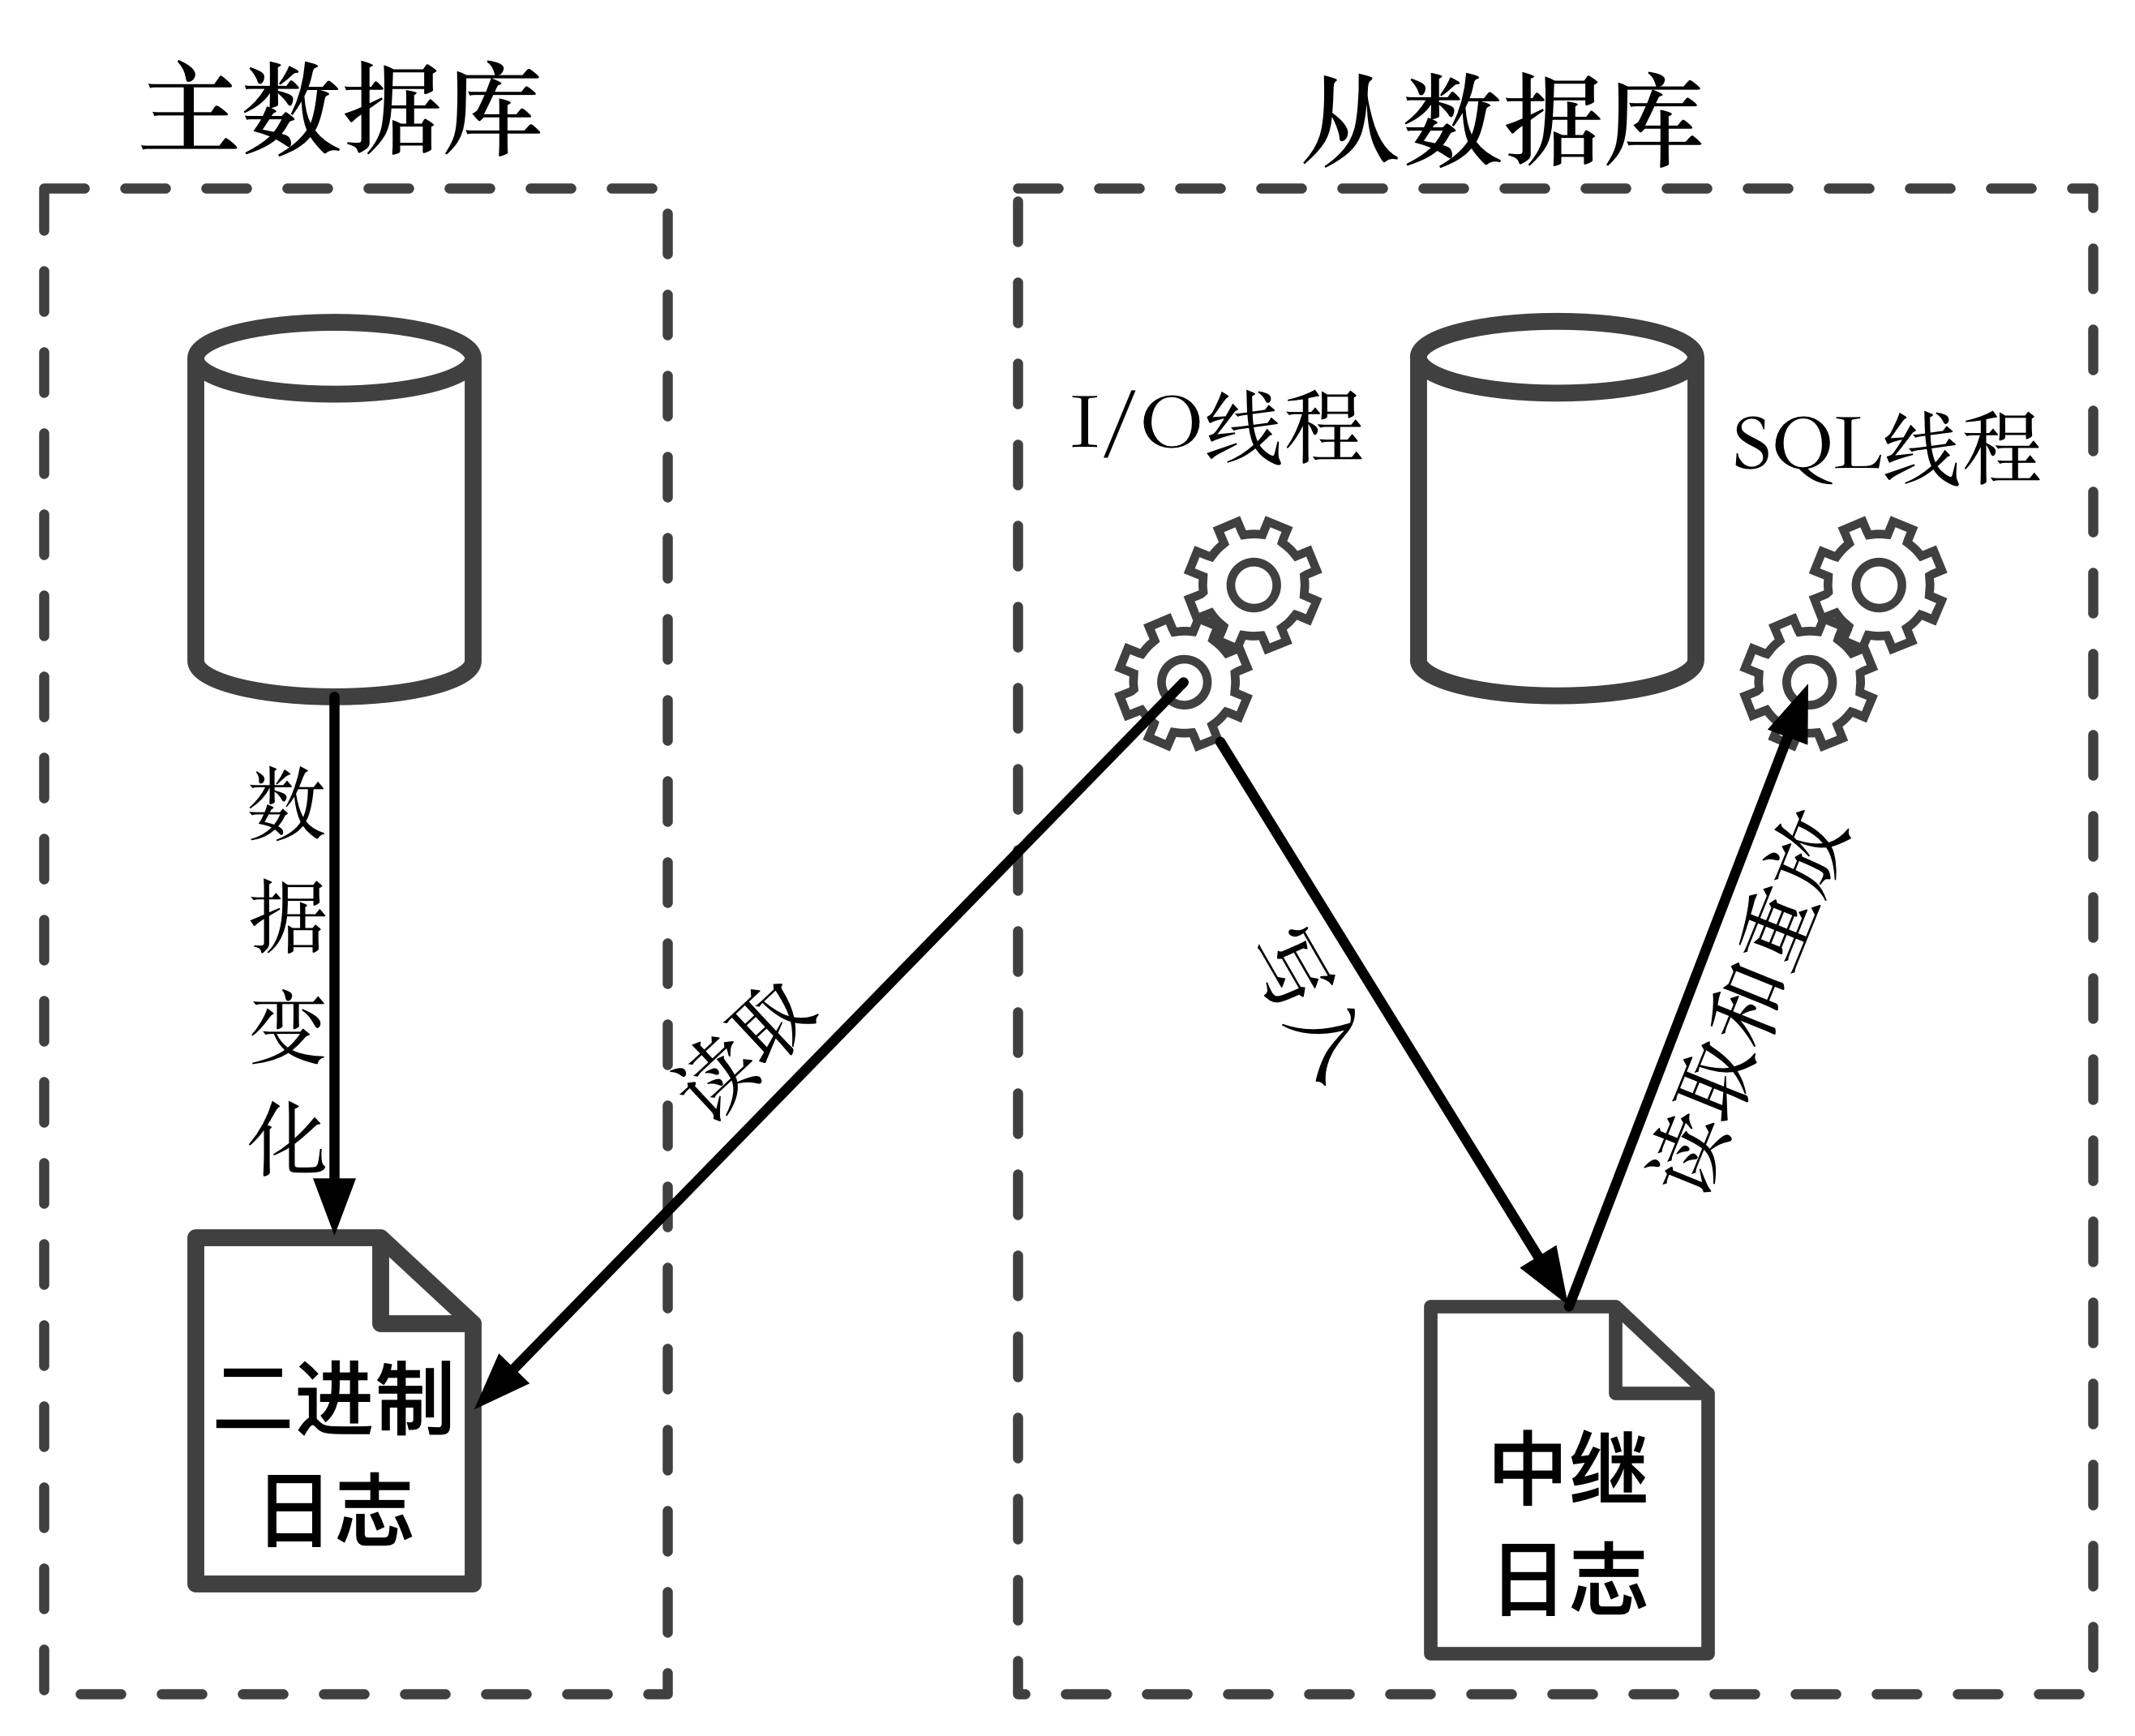
\includegraphics[width=4in]{chap04/replication2.png}
  \caption{MySQL复制流程}
  \label{fig:replication2}
\end{figure}
% 该过程的第一部分就是master记录二进制日志。在每个事务更新数据完成之前,master在二日志记录这些改变。MySQL将事务串行的写入二进制日志,即使事务中的语句都是交叉执行的。在事件写入二进制日志完成后,master通知存储引擎提交事务。

% 下一步就是slave将master的binary log拷贝到它自己的中继日志(relay log)。首先,slave开始一个工作线程——I/O线程。I/O线程在master上打开一个普通的连接,然后开始binlog dump process。Binlog dump process从master的二进制日志中读取事件,如果已经跟上master,它会睡眠并等待master产生新的事件。I/O线程将这些事件写入中继日志。

% SQL slave thread处理该过程的最后一步。SQL线程从中继日志读取事件,更新slave的数据,使其与master中的数据一致。只要该线程与I/O线程保持一致,中继日志通常会位于OS的缓存中,所以中继日志的开销很小。

% 此外,在master中也有一个工作线程:和其它MySQL的连接一样,slave在master中打开一个连接也会使得master开始一个线程。复制过程有一个很重要的限制——复制在slave上是串行化的,也就是说master上的并行更新操作不能在slave上并行操作\cite{秦金2013分布式}。

\subsection{双主复制设计}
目前生产环境的数据库有两个专有的服务器提供服务,为了保证数据的有效性和高可用性,两个服务器在同一时间只有一个提供数据业务服务,扮演主要的数据服务器角色,另外一个服务器复制主服务器的数据确保数据完整,扮演备服务器或从服务器角色。但是当主服务器出现问题而宕机时,需要快速的将从数据库切换为主数据库,在问题服务器恢复正常时作为从数据库,从新的主服务器复制数据。根据这个需求,将目前的两个数据库配置为双主数据库,将两个主数据库标示为master1和master2。

为了保证数据库的顺利复制,首先需要在两个数据库中通过stop slave命令来停止复制,并且保持两者的数据完全一致,通过reset master以及reset slave命令初始化。

然后在MySQl的配置文件中开启二进制日志,并为每一个数据库配置一个唯一的server-id,以及必要的配置。
\begin{lstlisting}[language=sql,numbers=none]
# 服务器ID
server-id = 1
# 开启二进制日志并配置日志名
log_bin = db2.bin
# 每一次事物提交都将binlog_cache中的数据强制写到磁盘
sync_binlog = 1
\end{lstlisting}
根据如上配置项,将两个数据库的二进制日志的文件名均配置为db2.bin,master1的server-id为1,master2的server-id为2,配置sync\_binlog 参数对MySQL数据库的运行性能和数据完整性非常重要,参数值设置为 1 表示在数据操作过程中我们每提交一次事务,数据库就会进行一次磁盘同步,将缓存中的数据写入磁盘中,提高数据的持久性。

除此之外,需要在配置文件中开启GTID
\begin{lstlisting}[language=sql,numbers=none]
# 开启gtid工作模式
gtid_mode = on
# 只允许能保障事物安全,且能够被日志记录的SQL语句被执行
enforce_gtid_consistency = 1
# 从库从主库复制数据时的操作也写入binlog
log_slave_updates
# 重启和启动时,如何迭代使用binlog文件
binlog_gtid_simple_recovery = 1
完成基本配置后,需要在数据库中配置和连接master。
\end{lstlisting}
GTID是全局事务标识(global transaction identifieds),在数据库中一个事务对应一个GTID,而且一个GTID在一个服务器上只执行一次,从而避免重复执行导致数据混乱或者主从不一致的情况,通过GTID可以保证日志文件中每一次事务都对应一个唯一的标志,对于从库拉取日志和进行日志分析具有很重要的意义。
\begin{enumerate}
\item 创建用于主从复制的用户
\begin{lstlisting}[numbers=none]
GRANT REPLICATION SLAVE ON *.* TO 'repl'@'%' IDENTIFIED BY 'replpassword';
\end{lstlisting}
其中repl为用户名,replpassword为密码
\item 配置master信息
\begin{lstlisting}[numbers=none]
change master to master_host ='ip', master_port = port, master_user = 'repl', master_password = 'replpassword', master_auto_position =1;
\end{lstlisting}
变量master\_host值为master所在服务器的IP地址,master\_port为master服务器的数据库连接端口,配置好用户名和密码。
master\_auto\_position让从库根据 GTID自动选择适当的事务点进行复制,基本上无需关注和担心主从不一致的问题。
\item 启动复制,并查看状态。
\begin{lstlisting}[language=sql,numbers=none]
start slave;
show slave status;
\end{lstlisting}
在查询结果的字段中通过Slave\_IO\_Running和Slave\_SQL\_Running两个变量的值为YES来判断主从复制是否成功启动。
\end{enumerate}

在master1和master2上均按照上述步骤进行操作,完成高可用的双主复制的部署。
\subsection{延迟复制设计}
为了避免上述服务器同时出现问题后无法提供数据服务的现象,论文考虑在本系统所使用的测试服务器中搭建一个延时复制服务器,延时复制的主库配置为master1,将复制策略配置为延迟1小时复制,然后通过二进制日志进行近一小时内数据的恢复,这样能够最大程度保证数据的完整。

配置的步骤基本类似于双主的配置,但是在配置master信息后需要增加一步,调整复制的延迟时间,单位是ms,因此一小时延时的变量值为3600。

\begin{lstlisting}[language=sql,numbers=none]
CHANGE MASTER TO MASTER_DELAY = 3600;
\end{lstlisting}

%\section{数据库负载均衡}
\section{数据库备份}
除了通过延迟复制来保证数据之外,服务器还将每天对数据库进行一次备份,并且将备份的数据库上传到阿里云的对象存储OSS中,目前master1和master2数据库的数据是一致的,因此只需要对master1的数据库进行备份即可。

通过mysqldump命令进行备份,备份完成之后通过阿里云OSS的Python SDK将备份文件上传到OSS中。

\begin{enumerate}
\item 开发OSS文件上传脚本

首先需要通过pip install oss2 命令在备份服务器中安装Python版本的OSS SDK,安装完成后在服务器的/mnt/sh中新建oss目录,并在oss目录下创建上传脚本dbuposs.py文件。修改文件如下:
\begin{lstlisting}[numbers=none]
#!/usr/bin/python2.7
import oss2
import sys
auth = oss2.Auth('AccessKeyId', 'AccessKeySecret ')
endpoint='http://oss-cn-beijing-internal.aliyuncs.com'
bucket = oss2.Bucket(auth, endpoint, 'mysqlbk')
bucket.put_object_from_file(sys.argv[1], '/mnt/mysqldump/'+sys.argv[1])
\end{lstlisting}
在脚本中配置阿里云OSS的访问域名(本项目的OSS访问域名为http://oss-cn-beijing-internal.aliyuncs.com),以及访问OSS的AccessKeyId和AccessKeySecret。配置完成之后即可完成访问OSS的认证工作。

通过oss2.Bucket函数连接OSS的mysqlbk存储空间获取bucket对象。

通过bucket对象的put\_object\_from\_file函数将指定的文件上传到OSS中,完成文件上传。
\item 开发数据库备份脚本

数据库脚本可以通过Shell脚本来实现,前提是需要在服务器中安装mysql,脚本的存放位置为/mnt/sh/mysqlbak.sh。

数据库备份脚本的设计流程为:
\begin{enumerate}
  \item 为了保证跟数据库服务器以及数据库服务的连接,首先需要配置服务器的基本信息和数据库相关信息,主要包括数据库服务器的IP地址以及数据库的服务端口号、数据库名称以及用于认证的用户名和密码等。
  \item 为了记录每次数据库备份的信息以及备份结果,需要在指定目录生成数据库备份日志文件,并且设计日志记录的内容和格式,确保每次备份都能准确的记录相关的信息,包括备份的时间、备份的结果、备份文件的路径及名称等。
  \item 为了保证数据库备份文件的有效空间占用和统一管理,配置备份文件的保存路径以及文件命名格式。
  \item 为了实现对多个数据表的分别备份,设计变量dbname数组,存放需要备份的数据表名称。
  \item 通过循环对需要备份的数据表进行备份,备份方式为:
  \begin{lstlisting}[numbers=none]
  mysqldump -u${dbuser} -p${dbpasswd} -hdbip -Pdbport ${dbn} --set-gtid-purged=OFF > ${logpath}/${backtime}.sql
  \end{lstlisting}
  通过mysqldump命令实现数据库的备份
  \item 为了节约磁盘空间,对备份完成后的数据库进行压缩,将sql文件压缩为bz2格式的文件,压缩比为1:12。
  \item 为了保证备份文件长久存在,通过OSS文件上传脚本将压缩后的备份文件上传到阿里云的OSS。
  \item 为了合理的配置本地的数据恢复以及磁盘空间,对七天以上的备份进行删除,只保留近期的备份数据。
\end{enumerate}

备份脚本参见附录~\ref{cha:MysqlBackup}:


\item 定时任务设置

为了保证每天都进行一次数据库备份操作,需要通过定时任务来保证数据库备份脚本每天执行一次。在Linux环境中,通过crontab软件来执行定时任务。crontab是一个在类Unix操作系统上的任务计划程序,它可以让用户在指定时间段周期性地运行命令或者shell脚本,通常被用在系统的自动化维护或者管理。

在本项目中,cron定时任务的配置文件在/var/spool/cron中的root文件,在root文件中添加如下定时任务:
\begin{lstlisting}[language=sh,numbers=none]
#<分钟> <小时> <日> <月份> <星期> <命令>
00 00 * * * /mnt/sh/mysqlbak.sh
\end{lstlisting}
设定在每天的凌晨0点0分执行数据库备份脚本。
\end{enumerate}
%\section{数据恢复方案}
\section{本章总结}

本章是对本论文中WEB项目的数据库进行优化的一些策略,主要包括通过InnoDB配置参数调整提升数据库自身的运行性能,通过配置主从复制以及延迟复制提升数据的稳定性和有效性,通过开发数据库定时备份脚本来实现数据库的每日备份。通过这些策略,在提升MySQL运行性能的同时也保证了数据的完整性和有效性,对于WEB应用的作用至关重要。
\chapter{服务监控与应急措施优化}
在本论文的第三章和第四章分别对应用性能方面和数据库方面进行了优化,在系统优化的过程中,除了提升应用性能和数据库性能这两方面之外,对于服务器中运行的服务进行监控检查和报警,并且能够实现自动化的Failover也是系统优化的重点,本章将对于目前项目开发过程中使用的工具和软件设计开发相应的监控脚本,并且探索在服务监控过程中的报警和故障恢复模式\cite{刘雄辉2007服务器监控管理}。
\label{cha:Monitor}
\section{阿里云云监控应用}
云监控(CloudMonitor)服务是由阿里云推出的,它的目的是对阿里云上的资源和互联网应用进行状态的监控。通过云监控服务,可以根据自定义规则获取阿里云资源的各项监控指标,可以通过设置服务的访问方式来探测服务的可用性,除此之外还可以对监控指标设置报警并及时通知运维人员。由于本项目的所有服务器均为阿里云服务器,所以一部分的监控可以通过配置阿里云资源的监控规则来对部分服务和资源状态进行监控,如对云服务器、云数据库和负载均衡等资源的监控,亦可以实现对使用HTTP和ICMP这些比较通用的网络协议的服务进行监控,保证网络服务的正常运行\cite{梁宇2014基于}。

在正式进行阿里云监控配置前,需要对目前阿里云资源进行统计,如表~\ref{tab:aliyun-resources}所示:

\begin{longtable}[c]{c*{2}{cp{7cm}}}
\caption{项目阿里云资源整理}\label{tab:aliyun-resources}\\
\toprule[1.5pt]
{\heiti 资源类别} & \multicolumn{1}{c}{\heiti 资源实例}  & {\heiti 资源介绍} \\\midrule[1pt]
\endfirsthead
\multicolumn{3}{c}{续表~\thetable\hskip1em 项目阿里云资源整理}\\
\toprule[1.5pt]
{\heiti 资源类别} & \multicolumn{1}{c}{\heiti 资源实例}  & {\heiti 资源介绍} \\\midrule[1pt]
\endhead
\hline
\multicolumn{3}{r}{续下页}
\endfoot
\endlastfoot
\multirow{5}*{站点} &  生产环境地址 & 生产环境应用的负载均衡入口地址  \\
                        &  测试环境地址 & 测试环境应用的负载均衡入口地址  \\
                        &  主数据库地址 & 生产环境主数据库的访问地址和端口  \\
                        &  从数据库地址 & 生产环境从数据库的访问地址和端口  \\
                        &  Couchbase地址  & 生产环境Couchbase入口地址\\
\hline
\multirow{5}*{云服务器ECS}  &  APP1 & WEB应用服务器,提供WEB应用服务  \\
                        &  APP2 & WEB应用服务器,提供WEB应用服务  \\
                        &  DB1 & 主数据库服务器,WEB请求的主服务器  \\
                        &  DB2 & 从数据库服务器,同DB1主从复制,DB1出现问题时切换为主数据库  \\
                        &  TEST & 测试服务器,提供测试环境相关的服务  \\
\hline
\multirow{3}*{负载均衡}  &  prod & 生产环境WEB应用负载均衡  \\
                        &  dbslb & 生产环境数据库负载均衡  \\
                        &  test & 测试环境负载均衡  \\
\multirow{3}*{CDN}  &  web & WEB应用访问域名  \\
                    &  img & 图片服务器域名  \\
                    &  fileserver & 文档服务器域名  \\
\bottomrule[1.5pt]
\end{longtable}

为了保证各个阿里云资源的正常使用,通过阿里云的云监控配置各服务的监控项,并且增加报警联系人,在监控到问题的时候能够通过短信或邮件的方式及时通知运维人员,以便在短时间内解决问题。
\begin{enumerate}

\item 站点监控

站点监控是指通过HTTP协议和TCP协议根据设置的监控频率去检测各个站点的访问时间,以此来判断站点是否正常。

对于生产环境的WEB应用和测试环境的WEB应用以及生产环境的Couchbase是通过HTTP协议去访问对应的地址。对于主从数据库则是通过TCP去测试数据库的链接是否正常。

监控的状态如图~\ref{fig:aliyun1}所示:
\begin{figure}[H] % use float package if you want it here
  \centering
  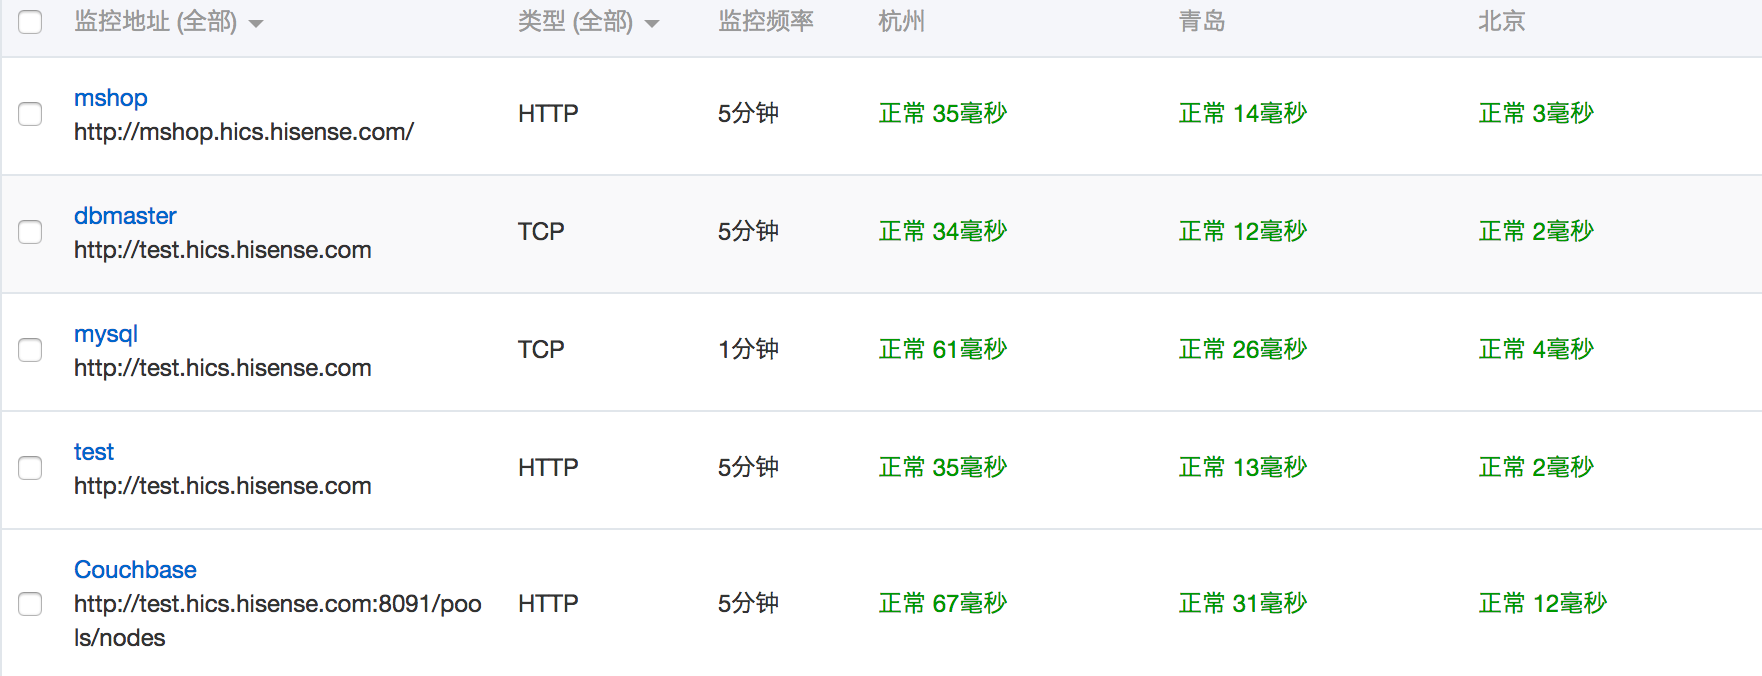
\includegraphics[width=6in]{chap05/aliyun1}
  \caption{站点监控状态图}
  \label{fig:aliyun1}
\end{figure}

\item 云服务器监控

云服务器的监控是指通过安装在服务器中的阿里云监控插件获取云服务器的状态,对于所有的云服务监控的规则都是一样的,均为CPU使用率、内存使用率和磁盘使用率三个方面,监控的具体规则如表~\ref{tab:aliyun-ecs}所示:
\begin{table}[H]
  \centering
  \begin{minipage}[t]{0.8\linewidth} % 如果想在表格中使用脚注,minipage是个不错的办法
  \caption[阿里云监控]{云服务器监控规则}
  \label{tab:aliyun-ecs}
    \begin{tabularx}{\linewidth}{lX}
      \toprule[1.5pt]
      {\heiti 监控项} & {\heiti 监控描述}\\\midrule[1pt]
        CPU使用率 & 5分钟 CPU使用率 平均值>85\% 则报警\\
        内存使用率 & 5分钟 内存使用率 最大值>95\% 则报警\\
        磁盘使用率 & 5分钟 磁盘使用率 平均值>70\% 则报警\\
      \bottomrule[1.5pt]
    \end{tabularx}
  \end{minipage}
\end{table}

\item 负载均衡监控

负载均衡主要是监控负载均衡内的各个服务器的监控状态以及负载均衡的带宽状态,当负载均衡出现异常时,可以通知报警联系人及时做出应对。
\begin{itemize}
\item 生产环境应用负载均衡监控规则
\begin{table}[H]
  \centering
  \begin{minipage}[t]{0.8\linewidth} % 如果想在表格中使用脚注,minipage是个不错的办法
  \caption[阿里云监控]{生产环境应用负载均衡监控规则}
  \label{tab:aliyun-slb1}
    \begin{tabularx}{\linewidth}{lX}
      \toprule[1.5pt]
      {\heiti 监控项} & {\heiti 监控描述}\\\midrule[1pt]
        流出带宽&5分钟 流出带宽 平均值>3M/s 则报警\\
        流入带宽&5分钟 流入带宽 平均值>3M/s 则报警\\
        后端异常ECS实例数&1分钟 后端异常ECS实例数 平均值>0个 则报警\\
      \bottomrule[1.5pt]
    \end{tabularx}
  \end{minipage}
\end{table}
\item 生产环境数据库负载均衡监控规则
\begin{table}[H]
  \centering
  \begin{minipage}[t]{0.8\linewidth} % 如果想在表格中使用脚注,minipage是个不错的办法
  \caption[阿里云监控]{生产环境数据库负载均衡监控规则}
  \label{tab:aliyun-slb2}
    \begin{tabularx}{\linewidth}{lX}
      \toprule[1.5pt]
      {\heiti 监控项} & {\heiti 监控描述}\\\midrule[1pt]
        后端健康ECS实例数&1分钟 后端健康ECS实例数 平均值<1个 则报警\\
      \bottomrule[1.5pt]
    \end{tabularx}
  \end{minipage}
\end{table}
\item 测试环境负载均衡监控规则
\begin{table}[H]
  \centering
  \begin{minipage}[t]{0.8\linewidth} % 如果想在表格中使用脚注,minipage是个不错的办法
  \caption[阿里云监控]{测试环境负载均衡监控规则}
  \label{tab:aliyun-slb3}
    \begin{tabularx}{\linewidth}{lX}
      \toprule[1.5pt]
      {\heiti 监控项} & {\heiti 监控描述}\\\midrule[1pt]
        流出带宽&5分钟 流出带宽 平均值>3M/s 则报警\\
        流入带宽&5分钟 流入带宽 平均值>3M/s 则报警\\
        后端异常ECS实例数&1分钟 后端异常ECS实例数 平均值>0个 则报警\\
      \bottomrule[1.5pt]
    \end{tabularx}
  \end{minipage}
\end{table}
\end{itemize}
\item CDN监控

CDN监控是指通过监控每一个域名的流量状态来判断应用的访问是否正常,当遇到DDos攻击时,CDN的流量会出现明显异常,通过监控这些异常,及时向运维人员报警,在很大程度上可以减少CDN流量的损失并降低被攻击的风险。

目前CDN监控的规则如表~\ref{tab:aliyun-cdn}所示:
\begin{table}[H]
  \centering
  \begin{minipage}[t]{0.8\linewidth} % 如果想在表格中使用脚注,minipage是个不错的办法
  \caption[阿里云监控]{CDN监控规则}
  \label{tab:aliyun-cdn}
    \begin{tabularx}{\linewidth}{lXX}
      \toprule[1.5pt]
      {\heiti 报警维度} & {\heiti 监控项} & {\heiti 监控描述}\\\midrule[1pt]
        fileserver&网络带宽峰值&5分钟 宽带峰值 平均值>4000000bit/s 则报警\\
        fileserver&公网下行流量&5分钟 公网网络出流量 求和值>100M/s 则报警\\
        img&网络带宽峰值&5分钟 宽带峰值 平均值>4000000bit/s 则报警\\
        web&网络带宽峰值&5分钟 宽带峰值 平均值>5000000bit/s 则报警\\
      \bottomrule[1.5pt]
    \end{tabularx}
  \end{minipage}
\end{table}
\end{enumerate}
\section{自定义服务监控}

虽然阿里云的云监控功能比较成熟,但是对于错误恢复和特殊需求的监控做的还相对不足,因此需要在本地的服务器中自己搭建监控环境,以提升系统的稳定性。

\subsection{心跳监听}

为了保证监控系统的高可用性,需要在APP1和APP2两个应用服务器内同时搭建监控系统,为了保证两套监控系统在同一时间只有一个监控系统在运行需要配置心跳监听,从监控节点通过心跳来监听主监控节点的运行状态,当主监控节点出现故障时,从监控节点运行监控进程,保证监控的正常\cite{巩天宁2012基于}。

Heartbeat是一款开源的提供高可用(Highly-Available)服务的软件,通过Heartbeat可以将资源(IP及程序服务等资源)从一台已经故障的计算机快速转移到另一台正常运转的机器上继续提供服务,称之为高可用服务。在实际生产应用场景中,heartbeat的功能和keepalived有很多相似之处,但在生产中,对实际的业务应用还是有区别的。如:keepalived主要是控制ip的漂移,配置、应用简单,而heartbeat则不但可以控制ip漂移,更擅长对资源服务的控制,配置、应用比较复杂~\cite{郭绪晶2012服务器集群系统高可用模块设计与实现}。由于Heartbeat能够对资源服务进行控制,所以本论文使用Heartbeat作为心跳监听的工具。

在服务器中配置心跳监听主要有以下步骤:
\begin{enumerate}
% \item 下载和安装Heartbeat软件

% 访问 http://www.linux-ha.org/wiki/Downloads 下载Heartbeat软件,解压完成后进入软件的目录中,执行以下命令完成安装:
% \begin{lstlisting}[language=sh,numbers=none]
% ./bootstrap
% #进入源码目录生成配置文件:
% ./ConfigureMe configure
% #编译安装
% make && make install
% \end{lstlisting}
% 安装完成后出现下面的信息表示安装成功:
% \begin{lstlisting}[numbers=none]
% heartbeat configuration:
%     Version                  = "3.0.6"
%     Executables              = "/usr/sbin"
%     Man pages                = "/usr/share/man"
%     Libraries                = "/usr/lib64"
%     Header files             = "/usr/include"
%     Arch-independent files   = "/usr/share"
%     Documentation files      = "/usr/share/doc/heartbeat"
%     State information        = "/var"
%     System configuration     = "/etc"
%     Init (rc) scripts        = "/etc/rc.d/init.d"
%     Init (rc) defaults       = "/etc/sysconfig"
%     Use system LTDL          = "yes"
%     HA group name            = "haclient"
%     HA group id              = "987"
%     HA user name             = "hacluster"
%     HA user user id          = "991"
%     Build dopd plugin        = "yes"
%     Enable times kludge      = "yes"
%     CC_WARNINGS              = " -Wall -Wmissing-prototypes -Wmissing-declarations -Wstrict-prototypes -Wdeclaration-after-statement -Wpointer-arith -Wwrite-strings -Wcast-qual -Wcast-align -Wbad-function-cast -Winline -Wmissing-format-attribute -Wformat=2 -Wformat-security -Wformat-nonliteral -Wno-long-long -Wno-strict-aliasing -Werror "
%     Mangled CFLAGS           = "-g -O2  -Wall -Wmissing-prototypes -Wmissing-declarations -Wstrict-prototypes -Wdeclaration-after-statement -Wpointer-arith -Wwrite-strings -Wcast-qual -Wcast-align -Wbad-function-cast -Winline -Wmissing-format-attribute -Wformat=2 -Wformat-security -Wformat-nonliteral -Wno-long-long -Wno-strict-aliasing -Werror  -ggdb3 -funsigned-char"
%     Libraries                = "-lbz2 -lz -lc -luuid -lrt -ldl  -lltdl"
%     RPATH enabled            = "no"
%     Distro-style RPMs        = "no"
% Note: If you use the 'make install' method for installation you
%     also need to adjust '/etc/passwd' and '/etc/group' manually.
% \end{lstlisting}
\item 配置Heartbeat软件,实现两个服务器的心跳监听

heartbeat 软件在使用时主要需要配置3个文件,分别是认证文件authkeys,配置文件ha.cf 和 资源文件haresources。authkeys主要配置节点之间的认证方式;ha.cf是主要的配置文件,配置节点信息、网络信息、监听频率等;haresources主要配置需要运行的程序或脚本。这里以app1/app2两节点为例,其IP分别是10.46.170.191/10.172.89.141,这里示例的配置文件为app1的,app2的参考app1配置即可。

ha.cf主配置文件配置项如表~\ref{tab:heartbeat}所示:
\begin{table}[H]
  \centering
  \begin{minipage}[t]{0.8\linewidth} % 如果想在表格中使用脚注,minipage是个不错的办法
  \caption[Heartbeat]{心跳监听主配置文件参数}
  \label{tab:heartbeat}
    \begin{tabularx}{\linewidth}{lXX}
      \toprule[1.5pt]
      {\heiti 参数项} & {\heiti 参数内容} & {\heiti 参数描述}\\\midrule[1pt]
      logfile  & /var/log/ha-log &  日志路径口\\
      keepalive  & 2 &  发送心跳报文的间隔,默认单位为秒 \\
      deadtime  & 30 & 认为对方宕掉的间隔时间 \\
      warntime & 10 &  认为对方可能宕掉的间隔时间\\
      initdead & 120 & 等待对方启动的最大时间\\
      udpport & 694 & 表示heartbeat广播/单播通讯使用的udp端口\\
      bcast & eth0 & 心跳所使用的网络接口\\
      ucast & eth0 10.172.89.141 & 单播通讯,对方网络接口及IP地址\\
      auto\_failback & on & 表示当主节点正常之后是否将资源/服务切换回来\\
      node & app1,app2 & 就是heartbeat集群中的节点信息 \\
      \bottomrule[1.5pt]
    \end{tabularx}
  \end{minipage}
\end{table}
% \begin{lstlisting}[numbers=none]
% # 日志路径
% logfile /var/log/ha-log
% # 发送心跳报文的间隔,默认单位为秒。
% keepalive 2
% # 认为对方宕掉的间隔时间。
% deadtime 30
% # 认为对方可能宕掉的间隔时间。
% warntime 10
% # 等待对方启动的最大时间。
% initdead 120
% # 表示heartbeat广播/单播通讯使用的udp端口。
% udpport 694
% # 心跳所使用的网络接口。
% bcast   eth0
% # 单播通讯,对方网络接口及IP地址。
% ucast eth0 10.172.89.141
% # 表示当主节点正常之后是否将资源/服务切换回来。
% auto_failback on
% # 就是heartbeat集群中的节点信息。
% node    app2
% node    app1
% \end{lstlisting}
在配置过程中将app1配置为主节点,当配置auto\_failback为off时,app1节点异常时app2会接管继续执行监控程序,app1节点恢复后也不会移交监控程序,当配置auto\_failback为on时,app1节点恢复后app2会将资源移交回app1.

authkeys主配置文件配置如下:
\begin{lstlisting}[numbers=none]
auth 2
#1 crc
2 sha1 mimaminishop
#3 md5 somewords
\end{lstlisting}
此文件为不同集群中 heartbeat 节点进行连接的认证文件, 不同集群中该文件采用的算法和密钥必须相同,认证方式有 3 种算法:crc方式、md5加密方式和sha1哈希方式。三种方式中 crc方式只能够校验节点间通信的校验数据包是否损坏,不能进行安全性认证; sha1/md5 两种方式需要进行安全性认证,它们通过一个密钥来进行认证。sha1和md5两种方式相比,sh1方式的资源消耗远小于md5方式,因此在大多数应用中建议使用 sha1 方式\cite{heartbeat配置说明}。

可以看出,示例中使用的是sha1算法,如果要换用其他算法只需要修改auth指令后面的数字,然后取消相应行的注释即可。另外,该文件的属性必须为600,否则heartbeat启动将失败。

haresources主配置文件配置如下:
\begin{lstlisting}[numbers=none]
app1 system_monitor
\end{lstlisting}
这表示Heartbeat启动时会执行资源路径中的system\_monitor脚本,实现服务的监控。

\item 配置监控脚本,实现服务的监控。

目前系统服务的监控主要包括系统服务状态的监控和系统数据库状态的监控,通过Heartbeat可以保证上述监控的高可用性;首先开发系统的监控脚本system\_monitor脚本,脚本的具体内容参见附录~\ref{cha:systemmonitor},通过脚本的内容可以看出在保证监控程序高可用的情况下,在监控频率上也进行相应的配置,将监控的频率设置为30s,表示监控程序每30秒会对所有的服务状态和数据库状态进行一次轮询检查,出现异常进行相应的处理,大大保证了监控的有效性。

监控脚本的主要流程和策略可以参见图~\ref{fig:systemmonitor},服务的监控主要是对Tomcat服务和MySQL服务的运行状态进行监控,数据库状态的监控主要是对数据库的主从同步状态进行监控,确保数据的完整性。
\begin{figure}[H] % use float package if you want it here
  \centering
  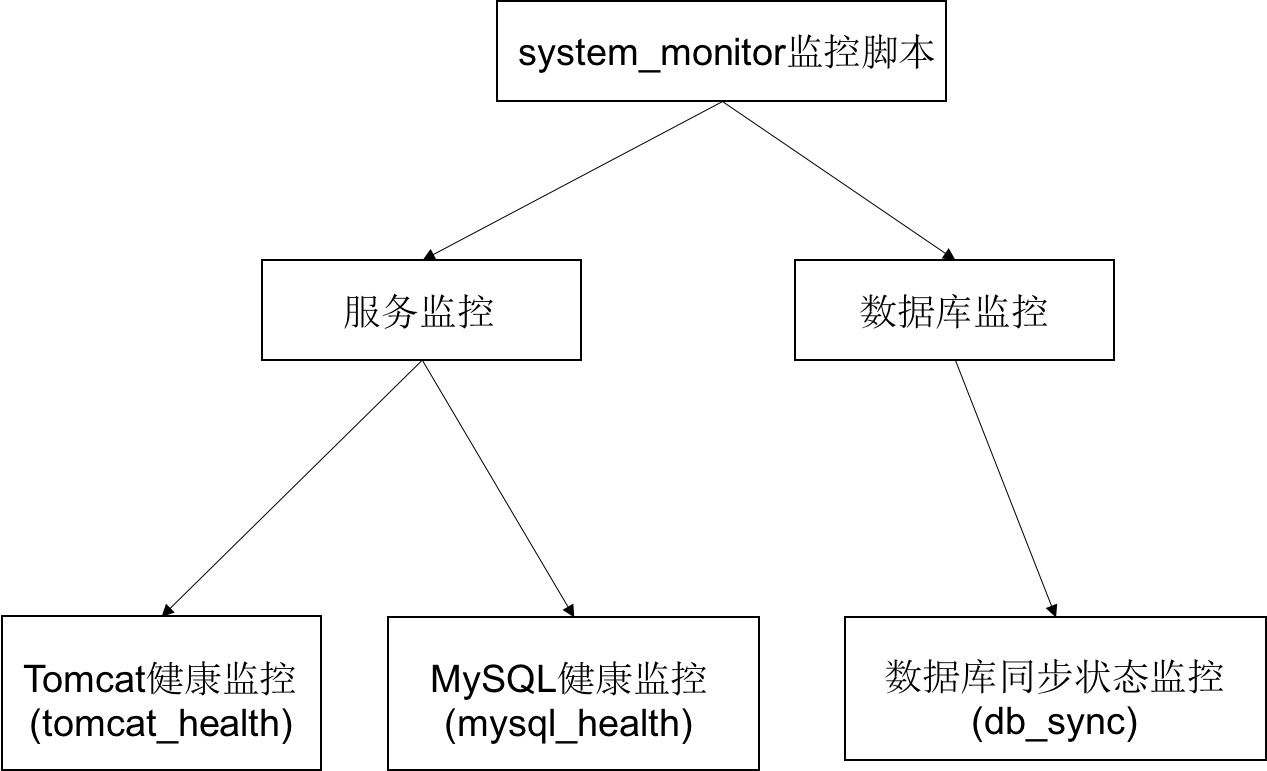
\includegraphics[width=5in]{chap05/monitor}
  \caption{系统监控方案}
  \label{fig:systemmonitor}
\end{figure}

监控脚本设计和开发完成后,通过在app1和app2两台服务器上同时部署监控脚本,这样在app1服务器出现故障的情况下,app2会获得app1故障的消息,自身启动监控脚本确保监控的正常运行。由于在上一部分我们在配置心跳监听时,将auto\_failback参数配置为on,这表示当app1服务器状态恢复正常后,app2会主动停止自身的监控程序,将监控程序移交给app1服务器,这样既保证了监控的正常运行也实现了监控的高可用。

通过system\_monitor脚本,每30秒对脚本中的监控服务进行一次监听,如果有新的监控脚本,可以在该脚本中配置其他脚本的路径并完成相关配置。
\end{enumerate}

\subsection{Tomcat监控方案设计}
Tomcat是应用运行的容器,要保证WEB应用的正常运行必须要先保证Tomcat服务的正常运行,正常情况下我们在小型项目的开发过程中可以通过访问服务器,执行CentOS系统自带的服务状态命令查看Tomcat服务的状态:
\begin{lstlisting}[numbers=none]
systemctl status tomcat
\end{lstlisting}
执行上述命令后,终端中会显示tomcat服务的运行状态情况,如图~\ref{fig:tomcatmonitor}所示:
\begin{figure}[H] % use float package if you want it here
  \centering
  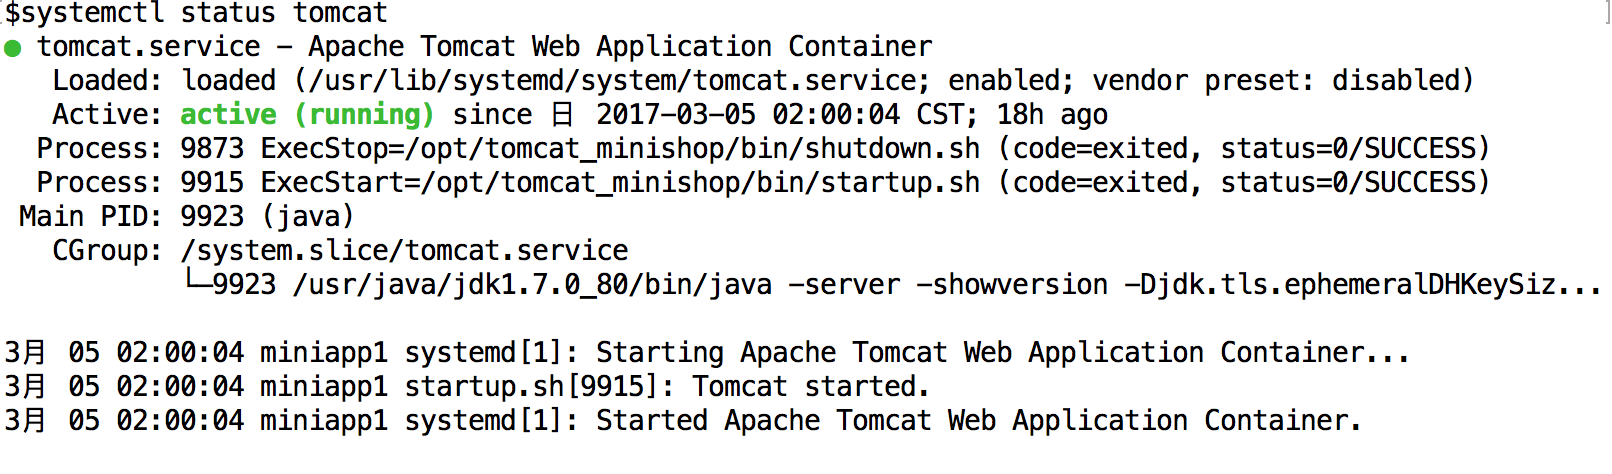
\includegraphics[width=5in]{chap05/tomcat}
  \caption{tomcat服务状态}
  \label{fig:tomcatmonitor}
\end{figure}
active(running)表示服务正常运行,除此之外还有其他的几种状态如表~\ref{tab:tomcat-status}所示:

\begin{table}[htb]
  \centering
  \begin{minipage}[t]{0.8\linewidth} % 如果想在表格中使用脚注,minipage是个不错的办法
  \caption[Tomcat]{Tocmat状态}
  \label{tab:tomcat-status}
    \begin{tabularx}{\linewidth}{lX}
      \toprule[1.5pt]
      {\heiti 状态} & {\heiti 描述}\\\midrule[1pt]
      active  &  运行正常  \\
      failed  &  启动失败  \\
      unknown &  未知错误\\
      \bottomrule[1.5pt]
    \end{tabularx}
  \end{minipage}
\end{table}

为了实现对于Tocmat的远程监控以及脚本监控,我们需要根据以上的几种运行状态去设计监控过程中对于Tomcat运行状态的判断和故障通知,除此之外,还需要使用可以通过SSH协议执行远程命令的Python库来实现在第三方服务器上开发Tomcat状态监控和通知的脚本。

综上,本论文选择Python的ssh库实现对于远程服务的ssh访问,通过ssh库中SSHClient()对象的connect方法可以建立本地对于远程服务器的连接,建立连接之后我们就可以执行远程命令了,这一部分同样通过ssh库的exec\_command函数来实现,通过该函数在被监控服务器端执行systemctl is-active tomcat.service命令来监测Tomcat服务的健康状态,根据不同的服务运行状态设计Python脚本返回的服务运行状态码,如表~\ref{tab:tomcat-code}所示:
\begin{table}[htb]
  \centering
  \begin{minipage}[t]{0.8\linewidth} % 如果想在表格中使用脚注,minipage是个不错的办法
  \caption[Tomcat]{自定义返回状态码}
  \label{tab:tomcat-code}
    \begin{tabularx}{\linewidth}{lX}
      \toprule[1.5pt]
      {\heiti 状态码} & {\heiti 描述}\\\midrule[1pt]
      100  &  表示WEB访问正常  \\
      101  &  表示WEB应用异常,需要查看日志  \\
      102  &  Tomcat服务停止,需要重启  \\
      103  &  服务不存在,需要查看日志\\
      104  &  服务器连接失败,需要查看是网络问题还是服务器异常  \\
      105  &  服务重启  \\
      106  &  其他异常\\
      200  &  重启成功  \\
      201  &  重启失败  \\
      \bottomrule[1.5pt]
    \end{tabularx}
  \end{minipage}
\end{table}

在Python监控脚本中,如果出现可以自动解决的问题比如服务停止的异常,可以通过执行远程命令systemctl restart tomcat.service命令来重新启动Tomcat服务,最终Python监控脚本将状态码返回到SHELL监控脚本中。

以上提到的Python监控脚本仅仅是对于Tomcat状态监控的脚本,在实际应用中除了状态监控以外我们还需要考虑到日志存储和短信通知的问题,这些问题我们通过设计一个shell监控脚本来实现日志记录和短信通知的功能。首先我们通过调用Python监控脚本,根据脚本返回的状态码来进行判断,然后根据判断结果进行日志的记录和短信通知。

综合上述介绍的两部分,Tomcat监控的框架可以描述为图~\ref{fig:tomcat-frame}所示:
\begin{figure}[H] % use float package if you want it here
  \centering
  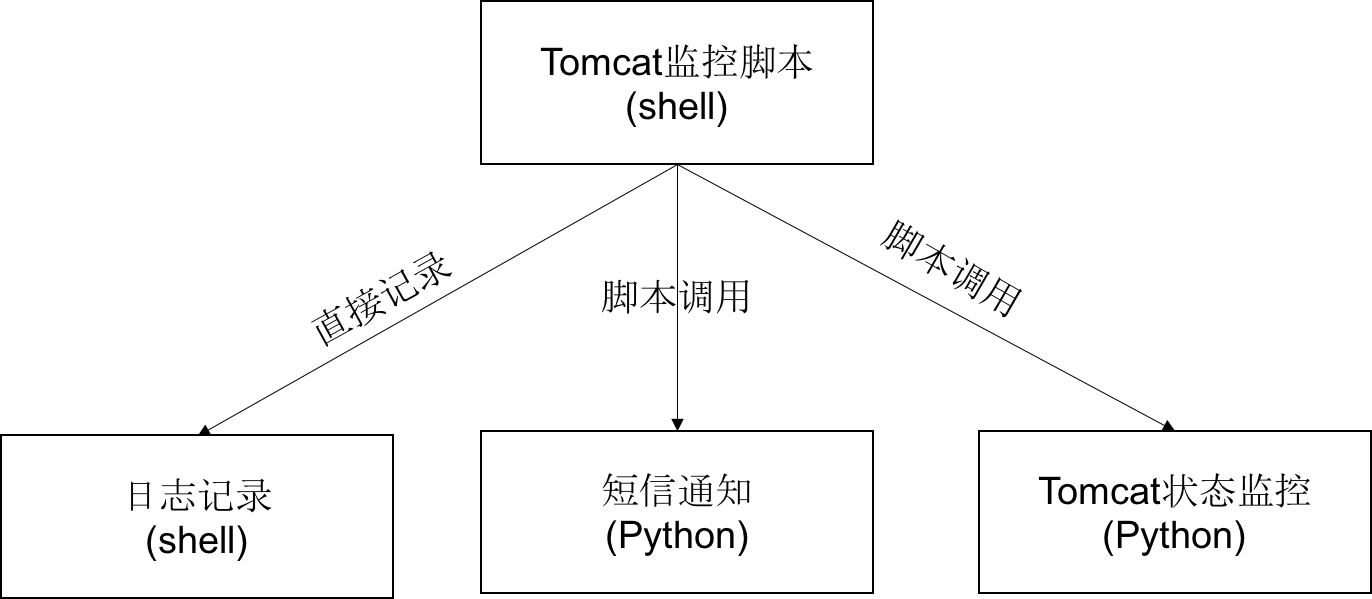
\includegraphics[width=5in]{chap05/tomcat2}
  \caption{Tomcat监控框架}
  \label{fig:tomcat-frame}
\end{figure}

具体的监控和故障处理脚本可以通过附录~\ref{cha:Tomcathealth}和附录~\ref{cha:Tomcatfailover}来查看。
\subsection{数据库监控方案设计}

除了WEB应用容器Tomcat容器的监控,对数据库的监控对于系统的稳定性来说也是非常重要的,为了最大程度的保证数据库的稳定性和数据的完整性,本论文对于数据库部分设计开发了相对应的监控方案,为了保证数据库服务的正常运行设计开发了数据库健康状态监控方案;为了保证数据的完整性和高可用性设计开发了主从数据库复制状态监控。

\begin{enumerate}
\item 数据库健康状态监控方案

对于数据库的健康状态监控,可以通过跟Tomcat监控方案类似的方法进行监控,但是考虑到执行SSH命令对于系统的安全性来说有一定程度的威胁,而且MySQL服务本身可以实现远程的连接与访问,因此本部分没有使用基于SSH协议的远程命令执行方案对数据库健康状态进行监控,而是采用执行本地mysql命令访问远程的数据库,通过执行sql语句的命令来实现数据库健康状态监控。这样做的优势在于"systemctl status " 命令可以判断MySQL服务是否正常运行,且执行效率高。缺点在于无法检查MySQL内部异常导致服务异常但是运行正常的现象。

对于MySQL而言,其自身的"show status"命令可以获取到MySQL运行时的相关参数,包括进程状态、连接状态、存储引擎状态等相关信息,通过对有效参数进行判断可以准确的获取MySQL的健康状态,如果有正常的数据返回则说明数据库运行正常,否则数据库的健康状态出现问题。当出现问题时,首先需要通知运维人员,为了实现通知功能本论文开发了短信通知的功能,这部分可以参考下一节,其次需要对当前的问题进行分析和判断,如果主从两台服务器的数据库的健康状态均出现问题,那么只能通过通知运维人员以人工介入的方式来解决问题,如果只有一台服务器的数据库健康状态出现问题,那么需要通过调整数据库负载均衡,将出现问题的数据库的权重设置为0,正常的数据库权重设置为100,保证数据库服务的正常运行,然后尝试重启异常的数据库服务进行故障恢复。

为了实现数据库负载均衡的动态调整,需要开发针对于阿里云负载均衡的权重调整脚本,通过分析和使用阿里云的负载均衡SDK来开发权重调整脚本,通过SDK的DescribeLoadBalancerAttributeRequest包来获取当前数据库负载均衡的状态,通过SetBackendServersRequest对负载均衡的权重进行调整,最终返回权重调整的结果。

为了实现数据库服务的远程重启,需要开发针对于Docker API的容器启动脚本,通过docker SDK的Client方法同远程服务器进行连接,通过inspect\_container方法获取远程容器的运行状态,如果MySQL容器的状态异常则通过restart方法进行重启。

综上所述,数据健康监控脚本的执行流程和顺序如图~\ref{fig:mysql-healty-monitor}所示。
\begin{figure}[H] % use float package if you want it here
  \centering
  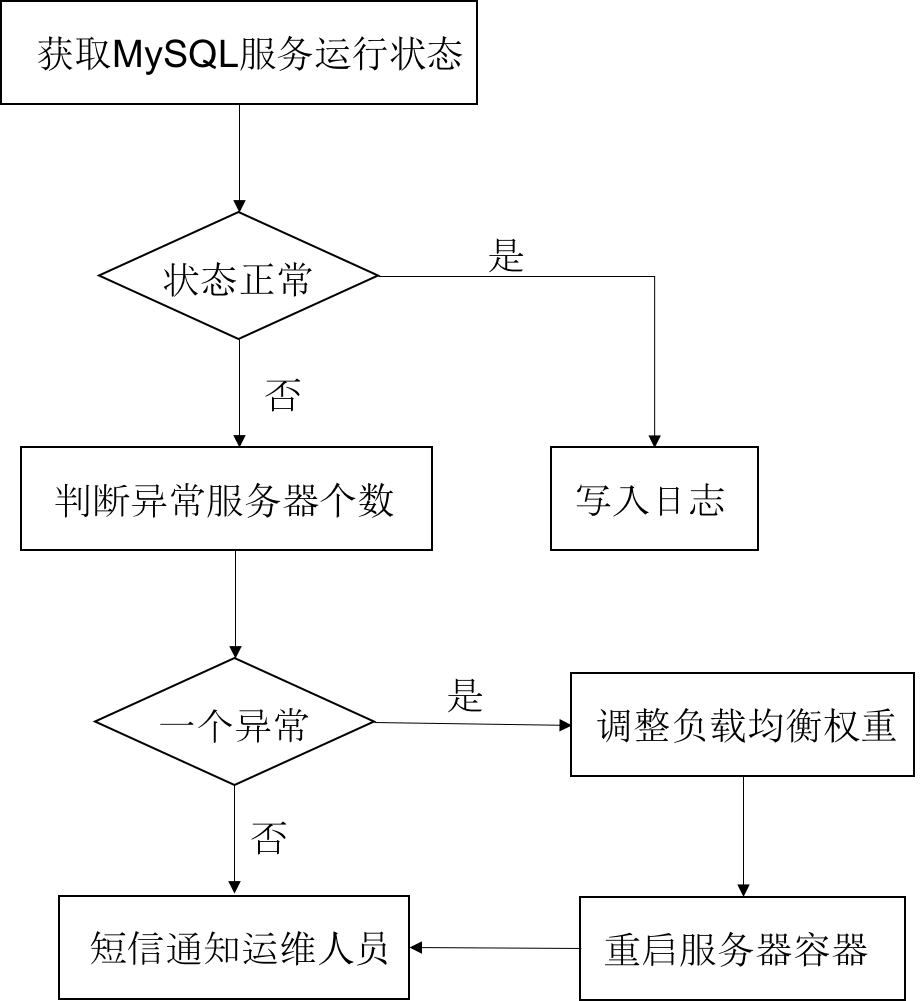
\includegraphics[width=5in]{chap05/mysql1}
  \caption{数据库健康状态监控方案}
  \label{fig:mysql-healty-monitor}
\end{figure}
完整的数据库健康监控脚本可以参考附录~\ref{cha:mysqlhealth}。

\item 数据库主从复制状态监控方案

针对数据库的主从数据库复制的问题性和数据一致性的问题,需要设计数据库主从复制状态监控方案,方案的目的就是通过执行主从复制的sql语句show slave status来获取数据库主从复制的状态,根据返回的参数值判断数据主从复制是否正常,如果正常则记录正常日志,否则需要将错误信息记录到日志文件中并短信通知运维人员。

对于执行show slave status语句后返回的数据库主从复制状态参数,主要通过以下三个方面判断数据库状态是否正常:
\begin{itemize}
  \item 通过Slave\_IO\_Running和Slave\_SQL\_Running两个参数的值来判断从库的复制状态是否正常,第一个参数负责与主机IO通信,第二个参数负责自己的slave mysql进程,如果两个参数的值均为YES则说明从库复制状态正常,否则说明复制状态不正常,需要检查从库的日志来进行问题的定位。这是进行数据库复制状态检查的第一步,只有以上两个参数值均为YES时才会进行下面的判断,否则直接将错误信息写入日志并短信通知运维人员。
  \item 通过Seconds\_Behind\_Master参数的值来判断主从复制的延迟,如果延迟时间大于300毫秒则说明主从复制状态异常,需要记录错误信息并短信通知运维人员,否则说明复制状态正常,需要进行下一步的判断。
  \item 通过Master\_Log\_File,Relay\_Master\_Log\_File,Read\_master\_log\_Pos和Exec\_Master\_log\_pos四个参数的值来判断主从复制的最终状态,其中Master\_Log\_File表示主库的数据库当前写入的日志文件,Relay\_Master\_Log\_File表示从库读取到的主库日志文件,如果两个参数一致则表示日志文件正常;Read\_master\_log\_Pos表示当前主库操作的日志位置,Exec\_Master\_log\_pos表示当前从库执行的主库日志位置,如果这两个参数一致则表示从库执行的最新操作是主库的最后操作,不存在延迟情况,只有当以上两种情况同时正常时,才会最终确认数据库主从复制正常,否则会将错误信息记录到日志文件中,并通知运维人员人工干预修复异常。
\end{itemize}

数据库主从复制状态监控的流程如图~\ref{fig:mysql-sync-monitor}所示。
\begin{figure}[H] % use float package if you want it here
  \centering
  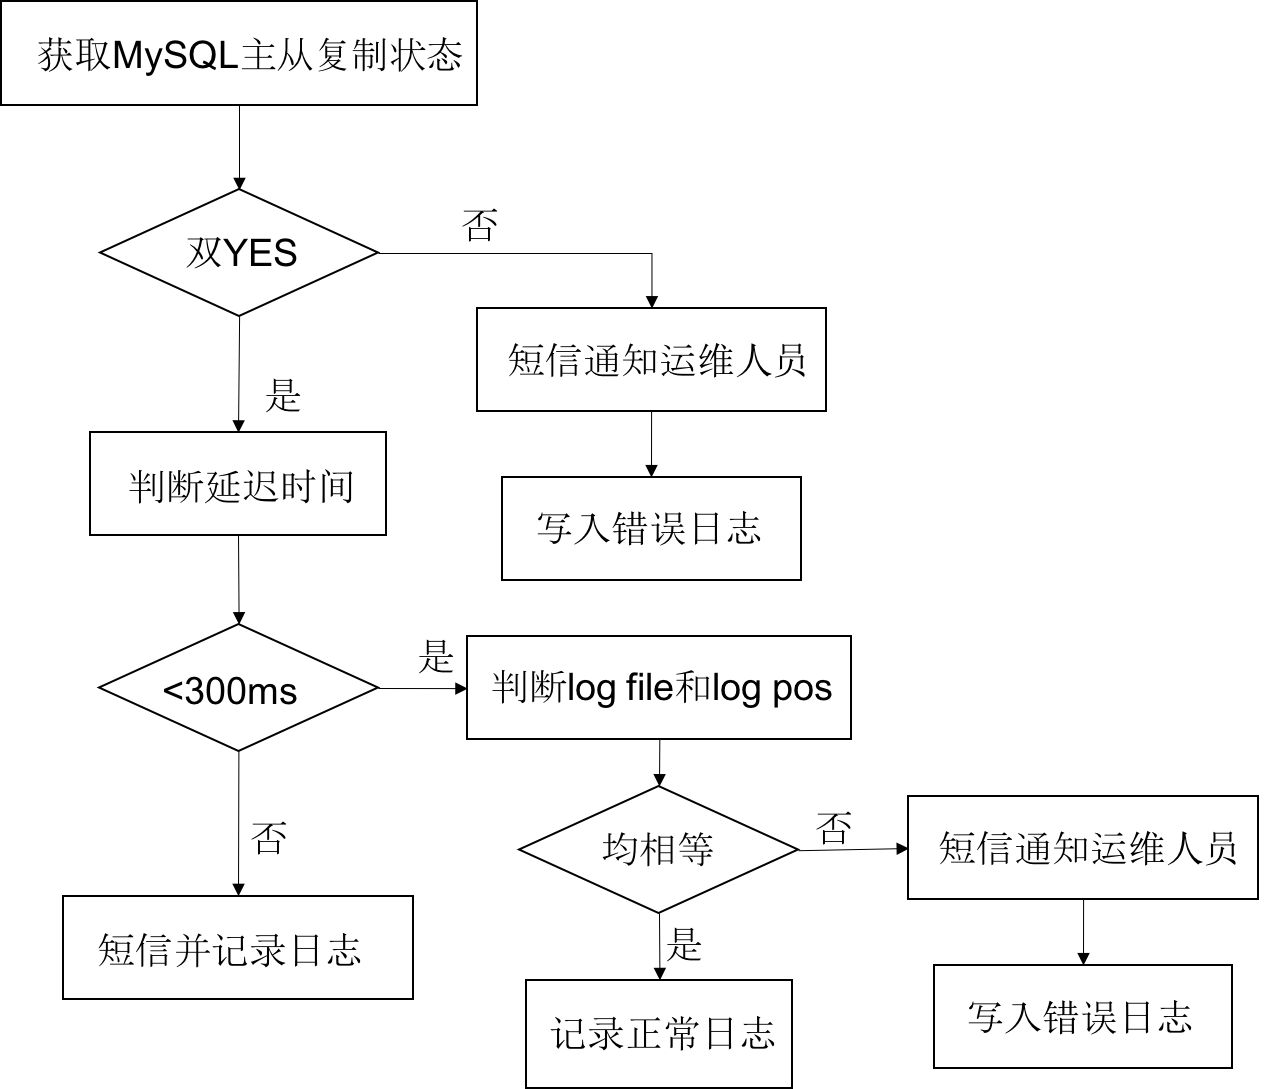
\includegraphics[width=5in]{chap05/mysql2}
  \caption{数据库主从复制状态监控方案}
  \label{fig:mysql-sync-monitor}
\end{figure}
数据库同步状态监控的脚本可以参考~\ref{cha:mysqlsync}。
\end{enumerate}

\section{短信通知方案设计}

在以前,当服务出现问题时无法及时的通知到运维人员,直到运维人员巡检或者应用的访问出现问题时运维人员才会发现故障,而现在有了监控的脚本,那么如何在第一时间通知运维人员就是需要解决的一大难题。通知时效性最高的就是短信通知,因此在服务器中开发一个能够发送短信的程序就显得非常重要\cite{陈泰伟2007基于短信平台的服务器监控系统关键技术探讨}。

为了实现短信的发送,首先需要选择和注册一个短信平台,因现有的云通讯平台短信发送的时间低于五秒,且支持自定义短信模版和支持API的特点,本论文选择云通讯作为系统的短信发送应用。

其次,需要在服务中安装SDK,同时开发短信发送脚本调用SDK以实现短信的发送,短信通知的脚本参考附录~\ref{cha:sms}。

在脚本中,首先需要根据自己注册的账户获取账户ID和验证Token,然后获取自己创建的应用的ID,完成基础的配置和认证。
在执行脚本时,通过SendTemplateSMS.py phone tempID content命令来发送短信,其中phone为接受短信的一个或者一组手机号,tempID为自己设计的短信模版对应的ID,contenet为短信的发送内容。

\section{日志备份方案设计}

在Tomcat的运行过程中,随着用户的访问,每天都会产生大量的访问日志和请求日志,随着时间的增加,日志的数量和空间占用会越来越大,为了解决日志的空间占用但又需要保证日志的存储以便后期进行日志分析的问题,需要设计开发日志备份脚本。主要的需求为:
\begin{itemize}
\item 每个月的1号会压缩上一个月的日志文件到压缩文件中
\item 每个月清理超过三个月的日志
\item 每个月压缩的日志上传到阿里云归档存储中进行备份
\end{itemize}
针对以上需求,开发的归档存储上传脚本参考附录~\ref{cha:aliyun-oas}。

通过oas库中oas\_api方法链接获取到OAS对象,通过对象的upload\_archive方法上传备份的日志文件。

开发的日志备份脚本可以参考附录~\ref{cha:Tomcatlog},脚本中首先通过匹配不同类型的日志名称来将日志文件分类压缩,然后通过执行OAS上传脚本上传压缩后的日志文件,上传完成后删除未压缩的日志文件。

日志备份脚本开发完成后,为了保证脚本每个月运行一次,需要修改crontab的配置文件,增加:
\begin{lstlisting}[numbers=none]
0 3 1 * * /opt/sh/Prod_tomcat_log_bak.sh
\end{lstlisting}
设置脚本执行时间为每个月1号的凌晨3点。
%\section{DockerAPI操作}
%\section{阿里云API优化}
\label{cha:Monitor-aliyun}
\section{本章总结}
本章主要对服务器层级的服务器监控措施和应急措施的优化策略研究,主要包括基于阿里云平台的自有监控和通知方案设计、个人开发的服务监控方案设计、短信通知脚本开发以及日志定期备份脚本开发等内容,通过以上的监控和优化措施,在最大程度上保证服务器和服务的正常运行、服务故障的自动恢复以及服务故障的通知,降低运维人员的时间成本,提升系统的稳定性。
\chapter{总结与展望}
\label{cha:summarize}
\section{总结}

本论文主要阐述了基于Spring MVC框架开发的WEB应用系统进行应用、数据库、服务器三个层级的优化研究,如图~\ref{fig:summery}所示。
\begin{figure}[H] % use float package if you want it here
  \centering
  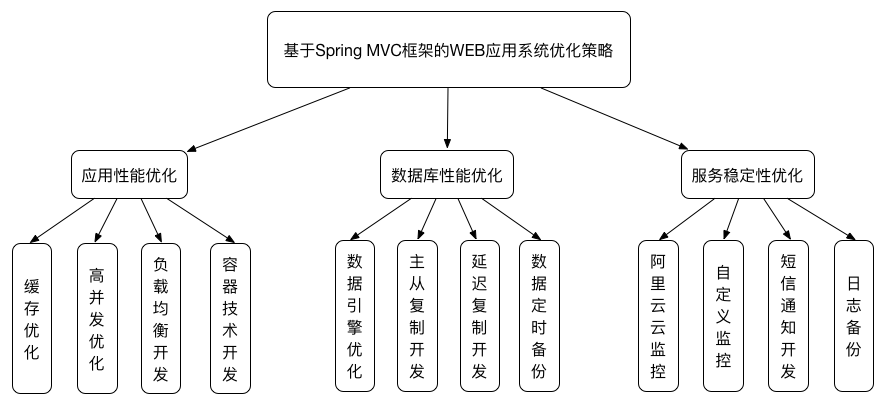
\includegraphics[width=6in]{chap06/summery}
  \caption{系统优化研究总结}
  \label{fig:summery}
\end{figure}

对于应用层面,论文通过开发Couchbase技术,将应用的基础数据缓存到Couchbase缓存中,提高了数据的加载效率并且降低了数据的压力;通过对Tomcat进行基于高并发的apr模块优化,大大提升了Tomcat对于用户请求的处理,提升了用户的访问速度;通过开发负载均衡技术,将用户的请求转发到两台应用服务器中,降低了服务器的压力,同时增强了应用的高可用性;通过开发Docker容器技术,将数据库应用、Couchbase应用以容器的方式提供服务,在新增加服务器节点的过程中提高了快速部署应用的效率,同时实现了多个服务器同一服务的集中管理,大大提高了运维人员的工作效率。

对于数据库层面,首先对数据库使用的数据引擎InnoDB引擎进行优化,在内存读取、日志、IO和其它方面提升了数据库的运行效率以及数据的稳定性;通过开发双主数据库的主从复制,提升了数据库的高可用性以及数据的完整性;通过开发延迟复制,可以最大程度的将数据进行备份,加上基于二进制日志的恢复方式,能够在短时间内完成数据的恢复,这对于提高数据的完整性和应用的用户体验尤为重要;通过开发数据定时备份脚本,将每日的数据进行备份,以避免数据丢失带来的数据损伤和经济损失。

对于服务器层面,论文通过阿里云的云监控服务,对系统的云服务器、负载均衡、网络站点以及CDN进行监控,当监控项出现异常时通知运维人员作出相应的处理,这提高了发现问题和解决服务器故障的效率,降低了过多流量丢失导致的经济损失;通过开发自定义监控实现对Tomcat服务的健康状态进行监测和重启,对MySQL的健康状态进行监测并根据监控情况调整数据库负载均衡损害数据库服务器的权重,并且短信通知运维人员,对于MySQL的主从同步状态进行监测并且通知运维人员;通过开发短信通知模块,实现重要信息的短信通知;通过日志备份模块的开发对Tomcat的运行日志进行定时备份并且上传到阿里云归档存储,方便运维人员在发生故障时的故障原因定位。

通过以上三个层面的优化策略研究,目前应用服务较优化前相比,单个服务器的负载达到了比较好的程度,应用的访问速度提升了接近20\%,新版的部署时间节省了50\%。

% 具体的数据对比在后期的论文完善过程中进行补充。

\section{展望}

虽然通过本论文的优化,WEB应用的性能得到了较大的提升,但是目前的WEB应用系统依然有很大的改进空间。
\begin{enumerate}

\item 搭建基于Nginx的前端服务器,由于Nginx在高并发的处理和静态文件的处理速度方面以及安全性方面的性能均优于Tomcat对静态页面的处理,因此搭建Nginx服务器处理用户的请求,将前端的页面请求直接提供给用户,后端的请求通过转发到Tomcat获取数据的处理结果。这样对于应用的访问速度还能进一步的提高,对于DDos攻击也能起到一定程度的防御\cite{reese2008nginx}。

\item 对于数据库的性能而言,除了自身的引擎提高之外,还可以通过读写分离来提高数据库的响应和降低数据库的负载\cite{刘进京2016mysql}。通过使用MaxScale插件,实现数据库请求的读写分离。具体的流程如图~\ref{fig:maxscale}所示。

\begin{figure}[H] % use float package if you want it here
  \centering
  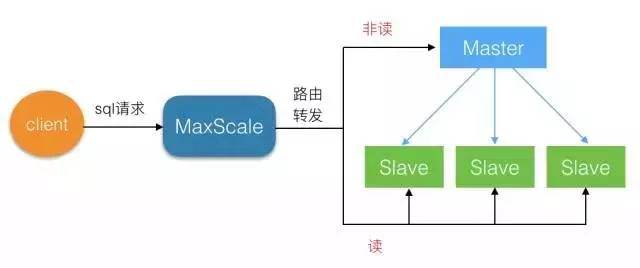
\includegraphics[width=5in]{chap06/maxscale}
  \caption{数据库读写分离流程}
  \label{fig:maxscale}
\end{figure}

MaxScale会根据用户的请求将读取的请求和非读取的请求转发到不同的数据库中,其中读取的请求转发到slave库中,其它请求转发到master库中,实现数据的读写分离。

\item 除了通过读写分离的方式提升数据库的效率以外,在数据库稳定性方面可以通过LiquiBase软件来实现数据库重构和迁移的操作,它可以在很大程度上保证当数据库之间出现数据不一致的情况时,能够自动的实现数据的同步和迁移,避免了人工干预导致的其它问题。

\item 本论文虽然用了阿里云的云监控实现了服务状态的监控,但是服务的自动failover工作却没有实现,目前还是通过人工干预来进行故障恢复。在以后的项目开发中,可以充分开发阿里云API的故障检测和自动failover系统,通过云监控的API去监控服务的状态,当出现故障时,自动调用failover程序通过故障服务的API接口进行故障的转移或者恢复,这对于提高故障的解决效率和WEB应用的高可用有更大的价值。

\end{enumerate}
%\chapter{绪论}
\label{cha:intro}

这是 \thuthesis{} 的示例文档,基本上覆盖了模板中所有格式的设置。建议大家在使用模
板之前,除了阅读《\thuthesis{}用户手册》,这个示例文档也最好能看一看。

小老鼠偷吃热凉粉;短长虫环绕矮高粱\footnote{韩愈(768-824),字退之,河南河阳(
  今河南孟县)人,自称郡望昌黎,世称韩昌黎。幼孤贫刻苦好学,德宗贞元八年进士。曾
  任监察御史,因上疏请免关中赋役,贬为阳山县令。后随宰相裴度平定淮西迁刑部侍郎,
  又因上表谏迎佛骨,贬潮州刺史。做过吏部侍郎,死谥文公,故世称韩吏部、韩文公。是
  唐代古文运动领袖,与柳宗元合称韩柳。诗力求险怪新奇,雄浑重气势。}。


\section{封面相关}
封面的例子请参看 cover.tex。主要符号表参看 denation.tex,附录和个人简历分别参看 appendix01.tex
和 resume.tex。里面的命令都很只管,一看即会\footnote{你说还是看不懂?怎么会呢?}。

\section{字体命令}
\label{sec:first}

苏轼(1037-1101),北宋文学家、书画家。字子瞻,号东坡居士,眉州眉山(今属四川)人
。苏洵子。嘉佑进士。神宗时曾任祠部员外郎,因反对王安石新法而求外职,任杭州通判,
知密州、徐州、湖州。后以作诗“谤讪朝廷”罪贬黄州。哲宗时任翰林学士,曾出知杭州、
颖州等,官至礼部尚书。后又贬谪惠州、儋州。北还后第二年病死常州。南宋时追谥文忠。
与父洵弟辙,合称“三苏”。在政治上属于旧党,但也有改革弊政的要求。其文汪洋恣肆,
明白畅达,为“唐宋八大家”之一。  其诗清新豪健,善用夸张比喻,在艺术表现方面独具
风格。少数诗篇也能反映民间疾苦,指责统治者的奢侈骄纵。词开豪放一派,对后代很有影
响。《念奴娇·赤壁怀古》、《水调歌头·丙辰中秋》传诵甚广。

{\kaishu 坡仙擅长行书、楷书,取法李邕、徐浩、颜真卿、杨凝式,而能自创新意。用笔丰腴
  跌宕,有天真烂漫之趣。与蔡襄、黄庭坚、米芾并称“宋四家”。能画竹,学文同,也喜
  作枯木怪石。论画主张“神似”,认为“论画以形似,见与儿童邻”;高度评价“诗中有
  画,画中有诗”的艺术造诣。诗文有《东坡七集》等。存世书迹有《答谢民师论文帖》、
  《祭黄几道文》、《前赤壁赋》、《黄州寒食诗帖》等。  画迹有《枯木怪石图》、《
  竹石图》等。}

{\fangsong 易与天地准,故能弥纶天地之道。仰以观於天文,俯以察於地理,是故知幽明之故。原
  始反终,故知死生之说。精气为物,游魂为变,是故知鬼神之情状。与天地相似,故不违。
  知周乎万物,而道济天下,故不过。旁行而不流,乐天知命,故不忧。安土敦乎仁,故
  能爱。范围天地之化而不过,曲成万物而不遗,通乎昼夜之道而知,故神无方而易无体。}

% 非本科生一般用不到幼圆与隶书字体。需要的同学请查看 ctex 文档。
{\ifcsname youyuan\endcsname\youyuan\else[无 \cs{youyuan} 字体。]\fi 有天地,然后
  万物生焉。盈天地之间者,唯万物,故受之以屯;屯者盈也,屯者物之始生也。物生必蒙,
  故受之以蒙;蒙者蒙也,物之穉也。物穉不可不养也,故受之以需;需者饮食之道也。饮
  食必有讼,故受之以讼。讼必有众起,故受之以师;师者众也。众必有所比,故受之以比;
  比者比也。比必有所畜也,故受之以小畜。物畜然后有礼,故受之以履。}

{\heiti 履而泰,然后安,故受之以泰;泰者通也。物不可以终通,故受之以否。物不可以终
  否,故受之以同人。与人同者,物必归焉,故受之以大有。有大者不可以盈,故受之以谦。
  有大而能谦,必豫,故受之以豫。豫必有随,故受之以随。以喜随人者,必有事,故受
  之以蛊;蛊者事也。}

{\ifcsname lishu\endcsname\lishu\else[无 \cs{lishu} 字体。]\fi 有事而后可大,故受
  之以临;临者大也。物大然后可观,故受之以观。可观而后有所合,故受之以噬嗑;嗑者
  合也。物不可以苟合而已,故受之以贲;贲者饰也。致饰然后亨,则尽矣,故受之以剥;
  剥者剥也。物不可以终尽,剥穷上反下,故受之以复。复则不妄矣,故受之以无妄。}

{\songti 有无妄然后可畜,故受之以大畜。物畜然后可养,故受之以颐;颐者养也。不养则不
  可动,故受之以大过。物不可以终过,故受之以坎;坎者陷也。陷必有所丽,故受之以
  离;离者丽也。}

\section{表格样本}
\label{chap1:sample:table} 

\subsection{基本表格}
\label{sec:basictable}

模板中关于表格的宏包有三个: \pkg{booktabs}、\pkg{array} 和
\pkg{longtabular},命令有一个 \cs{hlinewd}。三线表可以用 \pkg{booktabs}
提供的 \cs{toprule}、\cs{midrule} 和 \cs{bottomrule}。它们与
\pkg{longtable} 能很好的配合使用。如果表格比较简单的话可以直接用命令
\cs{hlinewd}\marg{width} 控制。
\begin{table}[htb]
  \centering
  \begin{minipage}[t]{0.8\linewidth} % 如果想在表格中使用脚注,minipage是个不错的办法
  \caption[模板文件]{模板文件。如果表格的标题很长,那么在表格索引中就会很不美
    观,所以要像 chapter 那样在前面用中括号写一个简短的标题。这个标题会出现在索
    引中。}
  \label{tab:template-files}
    \begin{tabularx}{\linewidth}{lX}
      \toprule[1.5pt]
      {\heiti 文件名} & {\heiti 描述} \\\midrule[1pt]
      thuthesis.ins & \LaTeX{} 安装文件,\textsc{DocStrip}\footnote{表格中的脚注} \\
      thuthesis.dtx & 所有的一切都在这里面\footnote{再来一个}。\\
      thuthesis.cls & 模板类文件。\\
      thuthesis.cfg & 模板配置文。cls 和 cfg 由前两个文件生成。\\
      thuthesis.bst    & 参考文献 BIB\TeX\ 样式文件。\\
      thuthesis.sty   & 常用的包和命令写在这里,减轻主文件的负担。\\
      \bottomrule[1.5pt]
    \end{tabularx}
  \end{minipage}
\end{table}

首先来看一个最简单的表格。表 \ref{tab:template-files} 列举了本模板主要文件及其功
能。请大家注意三线表中各条线对应的命令。这个例子还展示了如何在表格中正确使用脚注。
由于 \LaTeX{} 本身不支持在表格中使用 \cs{footnote},所以我们不得不将表格放在
小页中,而且最好将表格的宽度设置为小页的宽度,这样脚注看起来才更美观。

\subsection{复杂表格}
\label{sec:complicatedtable}

我们经常会在表格下方标注数据来源,或者对表格里面的条目进行解释。前面的脚注是一种
不错的方法,如果不喜欢脚注,可以在表格后面写注释,比如表~\ref{tab:tabexamp1}。
\begin{table}[htbp]
  \centering
  \caption{复杂表格示例 1}
  \label{tab:tabexamp1}
  \begin{minipage}[t]{0.8\textwidth} 
    \begin{tabularx}{\linewidth}{|l|X|X|X|X|}
      \hline
 \multirow{2}*{\diagbox[width=5em]{x}{y}} & \multicolumn{2}{c|}{First Half} & \multicolumn{2}{c|}{Second Half}\\\cline{2-5}
      & 1st Qtr &2nd Qtr&3rd Qtr&4th Qtr \\ \hline
      East$^{*}$ &   20.4&   27.4&   90&     20.4 \\
      West$^{**}$ &   30.6 &   38.6 &   34.6 &  31.6 \\ \hline
    \end{tabularx}\\[2pt]
    \footnotesize 注:数据来源《\thuthesis{} 使用手册》。\\
    *:东部\\
    **:西部
  \end{minipage}
\end{table}

此外,表~\ref{tab:tabexamp1} 同时还演示了另外两个功能:1)通过 \pkg{tabularx} 的
 \texttt{|X|} 扩展实现表格自动放大;2)通过命令 \cs{diagbox} 在表头部分
插入反斜线。

为了使我们的例子更接近实际情况,我会在必要的时候插入一些“无关”文字,以免太多图
表同时出现,导致排版效果不太理想。第一个出场的当然是我的最爱:风流潇洒、骏马绝尘、
健笔凌云的{\heiti 李太白}了。

李白,字太白,陇西成纪人。凉武昭王暠九世孙。或曰山东人,或曰蜀人。白少有逸才,志
气宏放,飘然有超世之心。初隐岷山,益州长史苏颋见而异之,曰:“是子天才英特,可比
相如。”天宝初,至长安,往见贺知章。知章见其文,叹曰:“子谪仙人也。”言于明皇,
召见金銮殿,奏颂一篇。帝赐食,亲为调羹,有诏供奉翰林。白犹与酒徒饮于市,帝坐沉香
亭子,意有所感,欲得白为乐章,召入,而白已醉。左右以水颒面,稍解,援笔成文,婉丽
精切。帝爱其才,数宴见。白常侍帝,醉,使高力士脱靴。力士素贵,耻之,摘其诗以激杨
贵妃。帝欲官白,妃辄沮止。白自知不为亲近所容,恳求还山。帝赐金放还。乃浪迹江湖,
终日沉饮。永王璘都督江陵,辟为僚佐。璘谋乱,兵败,白坐长流夜郎,会赦得还。族人阳
冰为当涂令,白往依之。代宗立,以左拾遗召,而白已卒。文宗时,诏以白歌诗、裴旻剑舞、
张旭草书为三绝云。集三十卷。今编诗二十五卷。\hfill —— 《全唐诗》诗人小传

浮动体的并排放置一般有两种情况:1)二者没有关系,为两个独立的浮动体;2)二者隶属
于同一个浮动体。对表格来说并排表格既可以像图~\ref{tab:parallel1}、图~\ref{tab:parallel2} 
使用小页环境,也可以如图~\ref{tab:subtable} 使用子表格来做。图的例子参见第~\ref{sec:multifig} 节。

\begin{table}[htbp]
\noindent\begin{minipage}{0.5\textwidth}
\centering
\caption{第一个并排子表格}
\label{tab:parallel1}
\begin{tabular}{p{2cm}p{2cm}}
\toprule[1.5pt]
111 & 222 \\\midrule[1pt]
222 & 333 \\\bottomrule[1.5pt]
\end{tabular}
\end{minipage}%
\begin{minipage}{0.5\textwidth}
\centering
\caption{第二个并排子表格}
\label{tab:parallel2}
\begin{tabular}{p{2cm}p{2cm}}
\toprule[1.5pt]
111 & 222 \\\midrule[1pt]
222 & 333 \\\bottomrule[1.5pt]
\end{tabular}
\end{minipage}
\end{table}

然后就是忧国忧民,诗家楷模杜工部了。杜甫,字子美,其先襄阳人,曾祖依艺为巩令,因
居巩。甫天宝初应进士,不第。后献《三大礼赋》,明皇奇之,召试文章,授京兆府兵曹参
军。安禄山陷京师,肃宗即位灵武,甫自贼中遁赴行在,拜左拾遗。以论救房琯,出为华州
司功参军。关辅饥乱,寓居同州同谷县,身自负薪采梠,餔糒不给。久之,召补京兆府功曹,
道阻不赴。严武镇成都,奏为参谋、检校工部员外郎,赐绯。武与甫世旧,待遇甚厚。乃于
成都浣花里种竹植树,枕江结庐,纵酒啸歌其中。武卒,甫无所依,乃之东蜀就高適。既至
而適卒。是岁,蜀帅相攻杀,蜀大扰。甫携家避乱荆楚,扁舟下峡,未维舟而江陵亦乱。乃
溯沿湘流,游衡山,寓居耒阳。卒年五十九。元和中,归葬偃师首阳山,元稹志其墓。天宝
间,甫与李白齐名,时称李杜。然元稹之言曰:“李白壮浪纵恣,摆去拘束,诚亦差肩子美
矣。至若铺陈终始,排比声韵,大或千言,次犹数百,词气豪迈,而风调清深,属对律切,
而脱弃凡近,则李尚不能历其藩翰,况堂奥乎。”白居易亦云:“杜诗贯穿古今,  尽工尽
善,殆过于李。”元、白之论如此。盖其出处劳佚,喜乐悲愤,好贤恶恶,一见之于诗。而
又以忠君忧国、伤时念乱为本旨。读其诗可以知其世,故当时谓之“诗史”。旧集诗文共六
十卷,今编诗十九卷。

\begin{table}[htbp]
\centering
\caption{并排子表格}
\label{tab:subtable}
\subcaptionbox{第一个子表格}
{
\begin{tabular}{p{2cm}p{2cm}}
\toprule[1.5pt]
111 & 222 \\\midrule[1pt]
222 & 333 \\\bottomrule[1.5pt]
\end{tabular}
}
\hskip2cm
\subcaptionbox{第二个子表格}
{
\begin{tabular}{p{2cm}p{2cm}}
\toprule[1.5pt]
111 & 222 \\\midrule[1pt]
222 & 333 \\\bottomrule[1.5pt]
\end{tabular}
}
\end{table}

不可否认 \LaTeX{} 的表格功能没有想象中的那么强大,不过只要足够认真,足够细致,
同样可以排出来非常复杂非常漂亮的表格。请参看表~\ref{tab:tabexamp2}。
\begin{table}[htbp]
  \centering\dawu[1.3]
  \caption{复杂表格示例 2}
  \label{tab:tabexamp2}
  \begin{tabular}[c]{|m{1.5cm}|c|c|c|c|c|c|}\hline
    \multicolumn{2}{|c|}{Network Topology} & \# of nodes & 
    \multicolumn{3}{c|}{\# of clients} & Server \\\hline
    GT-ITM & Waxman Transit-Stub & 600 &
    \multirow{2}{2em}{2\%}& 
    \multirow{2}{2em}{10\%}& 
    \multirow{2}{2em}{50\%}& 
    \multirow{2}{1.2in}{Max. Connectivity}\\\cline{1-3}
    \multicolumn{2}{|c|}{Inet-2.1} & 6000 & & & &\\\hline
    \multirow{2}{1.5cm}{Xue} & Rui  & Ni &\multicolumn{4}{c|}{\multirow{2}*{\thuthesis}}\\\cline{2-3}
    & \multicolumn{2}{c|}{ABCDEF} &\multicolumn{4}{c|}{} \\\hline
\end{tabular}
\end{table}

最后就是清新飘逸、文约意赅、空谷绝响的王大侠了。王维,字摩诘,河东人。工书画,与
弟缙俱有俊才。开元九年,进士擢第,调太乐丞。坐累为济州司仓参军,历右拾遗、监察御
史、左补阙、库部郎中,拜吏部郎中。天宝末,为给事中。安禄山陷两都,维为贼所得,服
药阳喑,拘于菩提寺。禄山宴凝碧池,维潜赋诗悲悼,闻于行在。贼平,陷贼官三等定罪,
特原之,责授太子中允,迁中庶子、中书舍人。复拜给事中,转尚书右丞。维以诗名盛于开
元、天宝间,宁薛诸王驸马豪贵之门,无不拂席迎之。得宋之问辋川别墅,山水绝胜,与道
友裴迪,浮舟往来,弹琴赋诗,啸咏终日。笃于奉佛,晚年长斋禅诵。一日,忽索笔作书
数纸,别弟缙及平生亲故,舍笔而卒。赠秘书监。宝应中,代宗问缙:“朕常于诸王坐闻维
乐章,今存几何?”缙集诗六卷,文四卷,表上之。敕答云,卿伯氏位列先朝,名高希代。
抗行周雅,长揖楚辞。诗家者流,时论归美。克成编录,叹息良深。殷璠谓维诗词秀调雅,
意新理惬。在泉成珠,著壁成绘。苏轼亦云:“维诗中有画,画中有诗也。”今编诗四卷。

要想用好论文模板还是得提前学习一些 \TeX/\LaTeX{}的相关知识,具备一些基本能力,掌
握一些常见技巧,否则一旦遇到问题还真是比较麻烦。我们见过很多这样的同学,一直以来
都是使用 Word 等字处理工具,以为 \LaTeX{}模板的用法也应该类似,所以就沿袭同样的思
路来对待这种所见非所得的排版工具,结果被折腾的焦头烂额,疲惫不堪。

如果您要排版的表格长度超过一页,那么推荐使用 \pkg{longtable} 或者 \pkg{supertabular}
宏包,模板对 \pkg{longtable} 进行了相应的设置,所以用起来可能简单一些。
表~\ref{tab:performance} 就是 \pkg{longtable} 的简单示例。
\begin{longtable}[c]{c*{6}{r}}
\caption{实验数据}\label{tab:performance}\\
\toprule[1.5pt]
 测试程序 & \multicolumn{1}{c}{正常运行} & \multicolumn{1}{c}{同步} & \multicolumn{1}{c}{检查点} & \multicolumn{1}{c}{卷回恢复}
& \multicolumn{1}{c}{进程迁移} & \multicolumn{1}{c}{检查点} \\
& \multicolumn{1}{c}{时间 (s)}& \multicolumn{1}{c}{时间 (s)}&
\multicolumn{1}{c}{时间 (s)}& \multicolumn{1}{c}{时间 (s)}& \multicolumn{1}{c}{
  时间 (s)}&  文件(KB)\\\midrule[1pt]
\endfirsthead
\multicolumn{7}{c}{续表~\thetable\hskip1em 实验数据}\\
\toprule[1.5pt]
 测试程序 & \multicolumn{1}{c}{正常运行} & \multicolumn{1}{c}{同步} & \multicolumn{1}{c}{检查点} & \multicolumn{1}{c}{卷回恢复}
& \multicolumn{1}{c}{进程迁移} & \multicolumn{1}{c}{检查点} \\
& \multicolumn{1}{c}{时间 (s)}& \multicolumn{1}{c}{时间 (s)}&
\multicolumn{1}{c}{时间 (s)}& \multicolumn{1}{c}{时间 (s)}& \multicolumn{1}{c}{
  时间 (s)}&  文件(KB)\\\midrule[1pt]
\endhead
\hline
\multicolumn{7}{r}{续下页}
\endfoot
\endlastfoot
CG.A.2 & 23.05 & 0.002 & 0.116 & 0.035 & 0.589 & 32491 \\
CG.A.4 & 15.06 & 0.003 & 0.067 & 0.021 & 0.351 & 18211 \\
CG.A.8 & 13.38 & 0.004 & 0.072 & 0.023 & 0.210 & 9890 \\
CG.B.2 & 867.45 & 0.002 & 0.864 & 0.232 & 3.256 & 228562 \\
CG.B.4 & 501.61 & 0.003 & 0.438 & 0.136 & 2.075 & 123862 \\
CG.B.8 & 384.65 & 0.004 & 0.457 & 0.108 & 1.235 & 63777 \\
MG.A.2 & 112.27 & 0.002 & 0.846 & 0.237 & 3.930 & 236473 \\
MG.A.4 & 59.84 & 0.003 & 0.442 & 0.128 & 2.070 & 123875 \\
MG.A.8 & 31.38 & 0.003 & 0.476 & 0.114 & 1.041 & 60627 \\
MG.B.2 & 526.28 & 0.002 & 0.821 & 0.238 & 4.176 & 236635 \\
MG.B.4 & 280.11 & 0.003 & 0.432 & 0.130 & 1.706 & 123793 \\
MG.B.8 & 148.29 & 0.003 & 0.442 & 0.116 & 0.893 & 60600 \\
LU.A.2 & 2116.54 & 0.002 & 0.110 & 0.030 & 0.532 & 28754 \\
LU.A.4 & 1102.50 & 0.002 & 0.069 & 0.017 & 0.255 & 14915 \\
LU.A.8 & 574.47 & 0.003 & 0.067 & 0.016 & 0.192 & 8655 \\
LU.B.2 & 9712.87 & 0.002 & 0.357 & 0.104 & 1.734 & 101975 \\
LU.B.4 & 4757.80 & 0.003 & 0.190 & 0.056 & 0.808 & 53522 \\
LU.B.8 & 2444.05 & 0.004 & 0.222 & 0.057 & 0.548 & 30134 \\
EP.A.2 & 123.81 & 0.002 & 0.010 & 0.003 & 0.074 & 1834 \\
EP.A.4 & 61.92 & 0.003 & 0.011 & 0.004 & 0.073 & 1743 \\
EP.A.8 & 31.06 & 0.004 & 0.017 & 0.005 & 0.073 & 1661 \\
EP.B.2 & 495.49 & 0.001 & 0.009 & 0.003 & 0.196 & 2011 \\
EP.B.4 & 247.69 & 0.002 & 0.012 & 0.004 & 0.122 & 1663 \\
EP.B.8 & 126.74 & 0.003 & 0.017 & 0.005 & 0.083 & 1656 \\
\bottomrule[1.5pt]
\end{longtable}

\subsection{其它}
\label{sec:tableother}
如果不想让某个表格或者图片出现在索引里面,请使用命令 \cs{caption*}。
这个命令不会给表格编号,也就是出来的只有标题文字而没有“表~XX”,“图~XX”,否则
索引里面序号不连续就显得不伦不类,这也是 \LaTeX{} 里星号命令默认的规则。

有这种需求的多是本科同学的英文资料翻译部分,如果觉得附录中英文原文中的表格和图
片显示成“表”和“图”不协调的话,一个很好的办法就是用 \cs{caption*},参数
随便自己写,比如不守规矩的表~1-111 和图~1-111 能满足这种特殊需要(可以参看附录部
分)。
\begin{table}[ht]
  \begin{minipage}{0.4\linewidth}
    \centering
    \caption*{表~1-111\quad 这是一个手动编号,不出现在索引中的表格。}
    \label{tab:badtabular}
      \framebox(150,50)[c]{\thuthesis}
  \end{minipage}%
  \hfill%
  \begin{minipage}{0.4\linewidth}
    \centering
    \caption*{Figure~1-111\quad 这是一个手动编号,不出现在索引中的图。}
    \label{tab:badfigure}
    \framebox(150,50)[c]{薛瑞尼}
  \end{minipage}
\end{table}

如果的确想让它编号,但又不想让它出现在索引中的话,目前模板上不支持。

最后,虽然大家不一定会独立使用小页,但是关于小页中的脚注还是有必要提一下。请看下
面的例子。

\begin{minipage}[t]{\linewidth-2\parindent}
  柳宗元,字子厚(773-819),河东(今永济县)人\footnote{山西永济水饺。},是唐代
  杰出的文学家,哲学家,同时也是一位政治改革家。与韩愈共同倡导唐代古文运动,并称
  韩柳\footnote{唐宋八大家之首二位。}。
\end{minipage}

唐朝安史之乱后,宦官专权,藩镇割据,土地兼并日渐严重,社会生产破坏严重,民不聊生。柳宗
元对这种社会现实极为不满,他积极参加了王叔文领导的“永济革新”,并成为这一
运动的中坚人物。他们革除弊政,打击权奸,触犯了宦官和官僚贵族利益,在他们的联合反
扑下,改革失败了,柳宗元被贬为永州司马。

\section{定理环境}
\label{sec:theorem}

给大家演示一下各种和证明有关的环境:

\begin{assumption}
待月西厢下,迎风户半开;隔墙花影动,疑是玉人来。
\begin{eqnarray}
  \label{eq:eqnxmp}
  c & = & a^2 - b^2\\
    & = & (a+b)(a-b)
\end{eqnarray}
\end{assumption}

千辛万苦,历尽艰难,得有今日。然相从数千里,未曾哀戚。今将渡江,方图百年欢笑,如
何反起悲伤?(引自《杜十娘怒沉百宝箱》)

\begin{definition}
子曰:「道千乘之国,敬事而信,节用而爱人,使民以时。」
\end{definition}

千古第一定义!问世间、情为何物,只教生死相许?天南地北双飞客,老翅几回寒暑。欢乐趣,离别苦,就中更有痴儿女。
君应有语,渺万里层云,千山暮雪,只影向谁去?

横汾路,寂寞当年箫鼓,荒烟依旧平楚。招魂楚些何嗟及,山鬼暗谛风雨。天也妒,未信与,莺儿燕子俱黄土。
千秋万古,为留待骚人,狂歌痛饮,来访雁丘处。

\begin{proposition}
 曾子曰:「吾日三省吾身 —— 为人谋而不忠乎?与朋友交而不信乎?传不习乎?」
\end{proposition}

多么凄美的命题啊!其日牛马嘶,新妇入青庐,奄奄黄昏后,寂寂人定初,我命绝今日,
魂去尸长留,揽裙脱丝履,举身赴清池,府吏闻此事,心知长别离,徘徊庭树下,自挂东南
枝。

\begin{remark}
天不言自高,水不言自流。
\begin{gather*}
\begin{split} 
\varphi(x,z)
&=z-\gamma_{10}x-\gamma_{mn}x^mz^n\\
&=z-Mr^{-1}x-Mr^{-(m+n)}x^mz^n
\end{split}\\[6pt]
\begin{align} \zeta^0&=(\xi^0)^2,\\
\zeta^1 &=\xi^0\xi^1,\\
\zeta^2 &=(\xi^1)^2,
\end{align}
\end{gather*}
\end{remark}

天尊地卑,乾坤定矣。卑高以陈,贵贱位矣。 动静有常,刚柔断矣。方以类聚,物以群分,
吉凶生矣。在天成象,在地成形,变化见矣。鼓之以雷霆,润之以风雨,日月运行,一寒一
暑,乾道成男,坤道成女。乾知大始,坤作成物。乾以易知,坤以简能。易则易知,简则易
从。易知则有亲,易从则有功。有亲则可久,有功则可大。可久则贤人之德,可大则贤人之
业。易简,而天下矣之理矣;天下之理得,而成位乎其中矣。

\begin{axiom}
两点间直线段距离最短。  
\begin{align}
x&\equiv y+1\pmod{m^2}\\
x&\equiv y+1\mod{m^2}\\
x&\equiv y+1\pod{m^2}
\end{align}
\end{axiom}

《彖曰》:大哉乾元,万物资始,乃统天。云行雨施,品物流形。大明始终,六位时成,时
乘六龙以御天。乾道变化,各正性命,保合大和,乃利贞。首出庶物,万国咸宁。

《象曰》:天行健,君子以自强不息。潜龙勿用,阳在下也。见龙再田,德施普也。终日乾
乾,反复道也。或跃在渊,进无咎也。飞龙在天,大人造也。亢龙有悔,盈不可久也。用九,
天德不可为首也。   

\begin{lemma}
《猫和老鼠》是我最爱看的动画片。
\begin{multline*}%\tag*{[a]} % 这个不出现在索引中
\int_a^b\biggl\{\int_a^b[f(x)^2g(y)^2+f(y)^2g(x)^2]
 -2f(x)g(x)f(y)g(y)\,dx\biggr\}\,dy \\
 =\int_a^b\biggl\{g(y)^2\int_a^bf^2+f(y)^2
  \int_a^b g^2-2f(y)g(y)\int_a^b fg\biggr\}\,dy
\end{multline*}
\end{lemma}

行行重行行,与君生别离。相去万余里,各在天一涯。道路阻且长,会面安可知。胡马依北
风,越鸟巢南枝。相去日已远,衣带日已缓。浮云蔽白日,游子不顾返。思君令人老,岁月
忽已晚。  弃捐勿复道,努力加餐饭。

\begin{theorem}\label{the:theorem1}
犯我强汉者,虽远必诛\hfill —— 陈汤(汉)
\end{theorem}
\begin{subequations}
\begin{align}
y & = 1 \\
y & = 0
\end{align}
\end{subequations}
道可道,非常道。名可名,非常名。无名天地之始;有名万物之母。故常无,欲以观其妙;
常有,欲以观其徼。此两者,同出而异名,同谓之玄。玄之又玄,众妙之门。上善若水。水
善利万物而不争,处众人之所恶,故几于道。曲则全,枉则直,洼则盈,敝则新,少则多,
多则惑。人法地,地法天,天法道,道法自然。知人者智,自知者明。胜人者有力,自胜
者强。知足者富。强行者有志。不失其所者久。死而不亡者寿。

\begin{proof}
燕赵古称多感慨悲歌之士。董生举进士,连不得志于有司,怀抱利器,郁郁适兹土,吾
知其必有合也。董生勉乎哉?

夫以子之不遇时,苟慕义强仁者,皆爱惜焉,矧燕、赵之士出乎其性者哉!然吾尝闻
风俗与化移易,吾恶知其今不异于古所云邪?聊以吾子之行卜之也。董生勉乎哉?

吾因子有所感矣。为我吊望诸君之墓,而观于其市,复有昔时屠狗者乎?为我谢
曰:“明天子在上,可以出而仕矣!” \hfill —— 韩愈《送董邵南序》
\end{proof}

\begin{corollary}
  四川话配音的《猫和老鼠》是世界上最好看最好听最有趣的动画片。
\begin{alignat}{3}
V_i & =v_i - q_i v_j, & \qquad X_i & = x_i - q_i x_j,
 & \qquad U_i & = u_i,
 \qquad \text{for $i\ne j$;}\label{eq:B}\\
V_j & = v_j, & \qquad X_j & = x_j,
  & \qquad U_j & u_j + \sum_{i\ne j} q_i u_i.
\end{alignat}
\end{corollary}

迢迢牵牛星,皎皎河汉女。
纤纤擢素手,札札弄机杼。
终日不成章,泣涕零如雨。
河汉清且浅,相去复几许。
盈盈一水间,脉脉不得语。

\begin{example}
  大家来看这个例子。
\begin{equation}
\label{ktc}
\left\{\begin{array}{l}
\nabla f({\mbox{\boldmath $x$}}^*)-\sum\limits_{j=1}^p\lambda_j\nabla g_j({\mbox{\boldmath $x$}}^*)=0\\[0.3cm]
\lambda_jg_j({\mbox{\boldmath $x$}}^*)=0,\quad j=1,2,\cdots,p\\[0.2cm]
\lambda_j\ge 0,\quad j=1,2,\cdots,p.
\end{array}\right.
\end{equation}
\end{example}

\begin{exercise}
  清列出 Andrew S. Tanenbaum 和 W. Richard Stevens 的所有著作。
\end{exercise}

\begin{conjecture} \textit{Poincare Conjecture} If in a closed three-dimensional
  space, any closed curves can shrink to a point continuously, this space can be
  deformed to a sphere.
\end{conjecture}

\begin{problem}
 回答还是不回答,是个问题。 
\end{problem}

如何引用定理~\ref{the:theorem1} 呢?加上 \cs{label} 使用 \cs{ref} 即可。妾发
初覆额,折花门前剧。郎骑竹马来,绕床弄青梅。同居长干里,两小无嫌猜。 十四为君妇,
羞颜未尝开。低头向暗壁,千唤不一回。十五始展眉,愿同尘与灰。常存抱柱信,岂上望夫
台。 十六君远行,瞿塘滟滪堆。五月不可触,猿声天上哀。门前迟行迹,一一生绿苔。苔深
不能扫,落叶秋风早。八月蝴蝶来,双飞西园草。感此伤妾心,坐愁红颜老。

\section{参考文献}
\label{sec:bib}
当然参考文献可以直接写 \cs{bibitem},虽然费点功夫,但是好控制,各种格式可以自己随意改
写。

本模板推荐使用 BIB\TeX,样式文件为 \texttt{thuthesis.bst},基本符合学校的参考文献格
式(如专利等引用未加详细测试)。看看这个例子,关于书的~\cite{tex, companion,
  ColdSources},还有这些~\cite{Krasnogor2004e, clzs, zjsw},关于杂志
的~\cite{ELIDRISSI94, MELLINGER96, SHELL02},硕士论文~\cite{zhubajie,
  metamori2004},博士论文~\cite{shaheshang, FistSystem01},标准文
件~\cite{IEEE-1363},会议论文~\cite{DPMG,kocher99},技术报告~\cite{NPB2},电子文
献~\cite{chuban2001,oclc2000}。中文参考文献~\cite{cnarticle}应增
加 \texttt{lang=``zh''} 字段,以便进行相应处理。另外,本模板对中文文
献~\cite{cnproceed}的支持并不是十全十美,如果有不如意的地方,请手动修
改 \texttt{bbl} 文件。

有时候不想要上标,那么可以这样~\inlinecite{shaheshang},这个非常重要。

有时候一些参考文献没有纸质出处,需要标注 URL。缺省情况下,URL 不会在连字符处断行,
这可能使得用连字符代替空格的网址分行很难看。如果需要,可以将模板类文件中
\begin{verbatim}
\RequirePackage{hyperref}
\end{verbatim}
一行改为:
\begin{verbatim}
\PassOptionsToPackage{hyphens}{url}
\RequirePackage{hyperref}
\end{verbatim}
使得连字符处可以断行。更多设置可以参考 \texttt{url} 宏包文档。

\section{公式}
\label{sec:equation}
贝叶斯公式如式~(\ref{equ:chap1:bayes}),其中 $p(y|\mathbf{x})$ 为后验;
$p(\mathbf{x})$ 为先验;分母 $p(\mathbf{x})$ 为归一化因子。
\begin{equation}
\label{equ:chap1:bayes}
p(y|\mathbf{x}) = \frac{p(\mathbf{x},y)}{p(\mathbf{x})}=
\frac{p(\mathbf{x}|y)p(y)}{p(\mathbf{x})} 
\end{equation}

论文里面公式越多,\TeX{} 就越 happy。再看一个 \pkg{amsmath} 的例子:
\newcommand{\envert}[1]{\left\lvert#1\right\rvert} 
\begin{equation}\label{detK2}
\det\mathbf{K}(t=1,t_1,\dots,t_n)=\sum_{I\in\mathbf{n}}(-1)^{\envert{I}}
\prod_{i\in I}t_i\prod_{j\in I}(D_j+\lambda_jt_j)\det\mathbf{A}
^{(\lambda)}(\overline{I}|\overline{I})=0.
\end{equation} 

前面定理示例部分列举了很多公式环境,可以说把常见的情况都覆盖了,大家在写公式的时
候一定要好好看 \pkg{amsmath} 的文档,并参考模板中的用法:
\begin{multline*}%\tag{[b]} % 这个出现在索引中的
\int_a^b\biggl\{\int_a^b[f(x)^2g(y)^2+f(y)^2g(x)^2]
 -2f(x)g(x)f(y)g(y)\,dx\biggr\}\,dy \\
 =\int_a^b\biggl\{g(y)^2\int_a^bf^2+f(y)^2
  \int_a^b g^2-2f(y)g(y)\int_a^b fg\biggr\}\,dy
\end{multline*}

其实还可以看看这个多级规划:
\begin{equation}\label{bilevel}
\left\{\begin{array}{l}
\max\limits_{{\mbox{\footnotesize\boldmath $x$}}} F(x,y_1^*,y_2^*,\cdots,y_m^*)\\[0.2cm]
\mbox{subject to:}\\[0.1cm]
\qquad G(x)\le 0\\[0.1cm]
\qquad(y_1^*,y_2^*,\cdots,y_m^*)\mbox{ solves problems }(i=1,2,\cdots,m)\\[0.1cm]
\qquad\left\{\begin{array}{l}
    \max\limits_{{\mbox{\footnotesize\boldmath $y_i$}}}f_i(x,y_1,y_2,\cdots,y_m)\\[0.2cm]
    \mbox{subject to:}\\[0.1cm]
    \qquad g_i(x,y_1,y_2,\cdots,y_m)\le 0.
    \end{array}\right.
\end{array}\right.
\end{equation}
这些跟规划相关的公式都来自于刘宝碇老师《不确定规划》的课件。

%\chapter{中华人民共和国}
\label{cha:china}

\section{其它例子}
\label{sec:other}

在第~\ref{cha:intro} 章中我们学习了贝叶斯公式~(\ref{equ:chap1:bayes}),这里我们复
习一下:
\begin{equation}
\label{equ:chap2:bayes}
p(y|\mathbf{x}) = \frac{p(\mathbf{x},y)}{p(\mathbf{x})}=
\frac{p(\mathbf{x}|y)p(y)}{p(\mathbf{x})}
\end{equation}

\subsection{绘图}
\label{sec:draw}

本模板不再预先装载任何绘图包(如 \pkg{pstricks,pgf} 等),完全由用户来决定。
个人觉得 \pkg{pgf} 不错,不依赖于 Postscript。此外还有很多针对 \LaTeX{} 的
 GUI 作图工具,如 XFig(jFig), WinFig, Tpx, Ipe, Dia, Inkscape, LaTeXPiX,
jPicEdt, jaxdraw 等等。

\subsection{插图}
\label{sec:graphs}

强烈推荐《\LaTeXe\ 插图指南》!关于子图形的使用细节请参看 \pkg{subcaption} 宏包的说明文档。

\subsubsection{一个图形}
\label{sec:onefig}
一般图形都是处在浮动环境中。之所以称为浮动是指最终排版效果图形的位置不一定与源文
件中的位置对应\footnote{This is not a bug, but a feature of \LaTeX!},这也是刚使
用 \LaTeX{} 同学可能遇到的问题。如果要强制固定浮动图形的位置,请使用 \pkg{float} 宏包,
它提供了 \texttt{[H]} 参数,比如图~\ref{fig:xfig1}。
\begin{figure}[H] % use float package if you want it here
  \centering
  
\includegraphics{thu-whole-logo}
  \caption{利用 Xfig 制图}
  \label{fig:xfig1}
\end{figure}

大学之道,在明明德,在亲民,在止于至善。知止而后有定;定而后能静;静而后能安;安
而后能虑;虑而后能得。物有本末,事有终始。知所先后,则近道矣。古之欲明明德于天
下者,先治其国;欲治其国者,先齐其家;欲齐其家者,先修其身;欲修其身者,先正其心;
欲正其心者,先诚其意;欲诚其意者,先致其知;致知在格物。物格而后知至;知至而后
意诚;意诚而后心正;心正而后身 修;身修而后家齐;家齐而后国治;国治而后天下
平。自天子以至于庶人,壹是皆以修身为本。其本乱而未治者 否矣。其所厚者薄,而其所
薄者厚,未之有也!

\hfill —— 《大学》


\subsubsection{多个图形}
\label{sec:multifig}

如果多个图形相互独立,并不共用一个图形计数器,那么
用 \texttt{minipage} 或者\texttt{parbox} 就可以。否则,请参看
图~\ref{fig:big1-subcaptionbox},它包含两个小图,分别是图~\ref{fig:subfig1}和
图~\ref{fig:subfig2}。推荐使用\cs{subcaptionbox},因为可以像
图~\ref{fig:big1-subcaptionbox} 那样对齐子图的标题,也可以使
用\pkg{subcaption}宏包的\cs{subcaption}(放在 minipage中,用法同\cs{caption})
或是 \pkg{subfigure} 、 \pkg{subtable}环境,像图~\ref{fig:big1-subfigure},
不要再用 \cs{subfloat}、\cs{subfigure} 和 \cs{subtable}。

\begin{figure}[h]
  \centering%
  \subcaptionbox{第一个小图形\label{fig:subfig1}}[3cm] %标题的长度,超过则会换行,如下一个小图。
    {
\includegraphics[height=3cm]{thu-fig-logo}}%
  \hspace{4em}%
  \subcaptionbox{第二个小图形,注意这个图略矮些。如果标题很长的话,它会自动换行\label{fig:subfig2}}
      {
\includegraphics[height=2cm]{thu-text-logo}}
  \caption{包含子图形的大图形(subcaptionbox示例)}
  \label{fig:big1-subcaptionbox}
\end{figure}
\begin{figure}[h]
  \centering%
  \begin{subfigure}{3cm}
    
\includegraphics[height=3cm]{thu-fig-logo}
    \caption{第一个小图形}
  \end{subfigure}%
  \hspace{4em}%
  \begin{subfigure}{0.5\textwidth}
    
\includegraphics[height=2cm]{thu-text-logo}
    \caption{第二个小图形,注意这个图略矮些。subfigure中同一行的子图在顶端对齐。}
  \end{subfigure}
  \caption{包含子图形的大图形(subfigure示例)}
  \label{fig:big1-subfigure}
\end{figure}

古之学者必有师。师者,所以传道受业解惑也。人非生而知之者,孰能无惑?惑而不从师,
其为惑也,终不解矣。生乎吾前,其闻道也固先乎吾,吾从而师之;生乎吾後,其闻道也亦
先乎吾,吾从而师之。吾师道也,夫庸知其年之先後生於吾乎!是故无贵无贱无长无少,道
之所存,师之所存也。

嗟乎!师道之不传也久矣,欲人之无惑也难矣。古之圣人,其出人也远矣,犹且从师而问焉;
今之众人,其下圣人也亦远矣,而耻学於师。是故圣益圣,愚益愚。圣人之所以为圣,愚
人之所以为愚,其皆出於此乎?爱其子,择师而教之,於其身也,则耻师焉,惑焉。彼童子
之师,授之书而习其句读者,非吾所谓传其道、解其惑者也。句读之不知,惑之不解,或师
焉,或不焉,小学而大遗,吾未见其明也。巫医、乐师、百工之人不耻相师,  士大夫之族
曰“师”曰“弟子”之云者,则群聚而笑之。问之,则曰:彼与彼年相若也,道相似也,位
卑则足羞,官盛则近谀。呜呼!师道之不复,可知矣。巫医、乐师、百工之人。吾子不齿,
今其智乃反不能及,其可怪也欤!圣人无常师。孔子师郯子、苌子、师襄、老聃。郯子之徒,
其贤不及孔子。孔子曰:“三人行,必有我师。”是故弟子不必不如师,师不必贤於弟子。
闻道有先後,术业有专攻,如是而已。

如果要把编号的两个图形并排,那么小页就非常有用了:
\begin{figure}
\begin{minipage}{0.48\textwidth}
  \centering
  
\includegraphics[height=2cm]{thu-whole-logo}
  \caption{并排第一个图}
  \label{fig:parallel1}
\end{minipage}\hfill
\begin{minipage}{0.48\textwidth}
  \centering
  
\includegraphics[height=2cm]{thu-whole-logo}
  \caption{并排第二个图}
  \label{fig:parallel2}
\end{minipage}
\end{figure}

李氏子蟠,年十七,好古文、六艺,经传皆通习之,不拘於时,学於余。余嘉其能行古
道,作师说以贻之。

\hfill —— 韩愈(唐)



%%% 其它部分
\backmatter

%% 本科生要这几个索引,研究生不要。选择性留下。
% 插图索引
%\listoffigures
% 表格索引
%\listoftables
% 公式索引
%\listofequations


%% 参考文献
% 注意:至少需要引用一篇参考文献,否则下面两行可能引起编译错误。
% 如果不需要参考文献,请将下面两行删除或注释掉。
\bibliographystyle{thuthesis}
\bibliography{ref/refs}


%% 附录
\begin{appendix}
% 
\chapter{其它附录}
前面两个附录主要是给本科生做例子。其它附录的内容可以放到这里,当然如果你愿意,可
以把这部分也放到独立的文件中,然后将其 \cs{input} 到主文件中。

\chapter{Tomcat健康监控脚本}
\label{cha:Tomcathealth}
\begin{lstlisting}[numbers=none]
#!/bin/bash
# func:执行SHELl命令监控tomcat服务状态并且执行重启操作
# author:武斌
# date:2017-01-23
# 修订历史:
# 创建--2017-01-23
# 调整检测时间--2017-02-01
# 基本变量配置
APP1_IP='10.46.170.191'
APP2_IP='10.172.89.141'
Error_Count=0
LOG_PATH="/tmp/tomcat_heal_stat.log"
#短信通知的手机号码
SMS_to='1766793****'
#短信通知的模版ID
SMS_tempId='86014'
function send_sms (){
    if [[ $sms_send_count_tomcat -lt 3 ]];then
        if [[ $sms_send_count_tomcat -lt 2 ]];then
            sms_send_count_tomcat=$[ sms_send_count_tomcat + 1 ]
        else
            sms_result=(python /opt/sh/sms/SendTemplateSMS.py ${SMS_to} ${SMS_tempId} $1)
            if [ "$?" == 0 ];then
                statusCode=${sms_result:0-6}
                if [ $statusCode == '000000' ];then
                    echo "----短信发送成功" >> $LOG_PATH
                    sms_send_count_tomcat=$[ sms_send_count_tomcat + 1 ]
                else
                    statusMsg=${sms_result##*Msg:}
                    statusMsg=${statusMsg%%s*}
                    echo "---短信发送失败,错误代码:${statusCode},错误信息:${statusMsg}" >> $LOG_PATH
                fi
            else
                echo "---短信发送失败" >> $LOG_PATH
            fi
        fi
    fi
}
function check_health () {
    check_result=(python /opt/sh/ssh/tomcat_fialover.py monitor $1)
    check_code="$?"
    if [[ $check_code -eq 100 ]];then
        echo "--[OK]$2 tomcat is RUNNING" >> $LOG_PATH
        TomcatServiceCode=$(curl -I -s -m 10 -o /dev/null  -w %{http_code} --connect-timeout 10 http://$1:8089/MiniShop/index.jsp)
        if [ $TomcatServiceCode -eq 200 ];then
            echo "--[OK]$2 WEB is OK" >> $LOG_PATH
            sms_send_count_tomcat=0
        else
            echo "--[ERROR]$2 tomcat页面出错,请注意......状态码为$TomcatServiceCode" >> $LOG_PATH
            message="$2:WEB页面访问出错,请查看。状态码为$TomcatServiceCode"
            send_sms $message
        fi
    elif [[ $check_code -eq 102 ]]; then
        echo "--[ERROR]$2 tomcat is STOPPING" >> $LOG_PATH
        echo "--[INFO]$2 开始重启Tomcat" >> $LOG_PATH
        restart_result=(python /opt/sh/ssh/tomcat_fialover.py restart $1)
        restart_code="$?"
        if [[ $restart_code -eq 200 ]]; then
            echo "--[OK]$2 Tomcat重启成功" >> $LOG_PATH
        else
            echo "--[ERROR]$2 Tomcat重启失败" >> $LOG_PATH
            message="$2:Tomcat重启失败"
            send_sms $message
        fi
    elif [[ $check_code -eq 103 ]]; then
        echo "--[ERROR]$2-Tomcat服务不存在" >> $LOG_PATH
        message="$2:Tomcat服务不存在"
        send_sms $message
    elif [[ $check_code -eq 104 ]]; then
        echo "--[ERROR]$2服务器连接失败" >> $LOG_PATH
        message="$2服务器连接失败"
        send_sms $message
    elif [[ $check_code -eq 105 ]]; then
        echo "--[ERROR]$2Tomcat正在重启" >> $LOG_PATH
    else
        echo "--[ERROR]$2未知错误:${check_result}" >> $LOG_PATH
        message="$2应用检测未知错误:${check_result}"
        send_sms $message
    fi
}
echo '####'(date '+%Y-%m-%d %H:%M:%S')####' >> $LOG_PATH
check_health ${APP1_IP} "APP1"
check_health ${APP2_IP} "APP2"
\end{lstlisting}
\chapter{Tomcat故障恢复脚本}
\label{cha:Tomcatfailover}
\begin{lstlisting}[language=python,numbers=none]
#!/usr/bin/python2.7
# -*- coding: utf-8 -*-

# func:执行SHELl命令监控tomcat服务状态并且执行重启操作
# author:武斌
# date:2017-01-23
# 修订历史:
# 创建--2017-01-23
import ssh
import sys

def main():
    try:
        if len(sys.argv) == 3:
            # 变量处理
            action=sys.argv[1]
            host=sys.argv[2]
            # 新建一个ssh客户端对象
            client=ssh.SSHClient()
            # 设置成默认自动接受密钥
            client.set_missing_host_key_policy(ssh.AutoAddPolicy())
            # 连接远程主机
            port=22
            username='root'
            key_filename = '/root/.ssh/id_rsa'
            client.connect(host, port=port, username=username, key_filename = key_filename)
            if action == 'monitor':
                stdin, stdout, stderr = client.exec_command("systemctl is-active tomcat.service")
                if stderr.read():
                    print stderr.read()
                    sys.exit(105)
                else:
                    status=stdout.read().strip()
                    if status == 'active':
                        print "运行正常"
                        sys.exit(100)
                    elif status == 'failed':
                        print "服务停止"
                        sys.exit(102)
                    elif status == 'unknown':
                        print "未知服务"
                        sys.exit(103)
                    elif status == 'deactivating':
                        print "服务重启"
                        sys.exit(105)
                    else:
                        print "未知状态"
                        sys.exit(106)
            elif action == 'restart':
                stdin, stdout, stderr = client.exec_command("systemctl restart tomcat.service")
                if stderr.read():
                    print stderr.read()
                    sys.exit(201)
                else:
                    print stdout.read()
                    sys.exit(200)
            else:
                print "不是有效参数"
                sys.exit(1)
        else:
            print "参数错误"
            sys.exit(1)
    except Exception:
        print "服务器连接出现问题,请联系管理员"
        sys.exit(104)
if __name__=='__main__':
    main()
\end{lstlisting}
\chapter{MySQL健康监控脚本}
\label{cha:mysqlhealth}
\begin{lstlisting}[numbers=none]
#!/bin/bash
# 基本变量配置
MYSQL='/usr/bin/mysql'
#MYSQL='/usr/local/mysql/bin/mysql'
DB1_HOST='hostname'
DB2_HOST='hostname'
DB1_USER='root'
DB2_USER='root'
DB1_PASSWORD='password'
DB2_PASSWORD='password'
DB1_PORT='3307'
DB2_PORT='3305'
MySQL_LOG_PATH="/tmp/mysql_heal_stat.log"
DB1_OK=1
DB2_OK=1
CHECK_TIME='30s'
CHECK_FLAG=0
DB1_BASE_URL='tcp://hostname:port'
DB2_BASE_URL='tcp://hostname:port'
DOCKER_API_VERSION='1.21'
MYSQL_CONTAINER_ID='dockermysql_mysql_1'
SMS_to='1766793****'
SMS_tempId='86014'
function check_db1_health (){
    $MYSQL -h${DB1_HOST} -u${DB1_USER} -p${DB1_PASSWORD} -P${DB1_PORT} -e "show status;" 1>/dev/null 2>&1
    if [ $? = 0 ] ;then
    DB1_OK=1
    else
    DB1_OK=0
    fi
    return $DB1_OK
}
function check_db2_health (){
    $MYSQL -h${DB2_HOST} -u${DB2_USER} -p${DB2_PASSWORD} -P${DB2_PORT} -e "show status;"  1>/dev/null 2>&1
    if [ $? = 0 ] ;then
    DB2_OK=1
    else
    DB2_OK=0
    fi
    return $DB2_OK
}
function send_sms (){
    if [[ $sms_send_count_1 -lt 1 ]];then
        sms_result=(python /opt/sh/sms/SendTemplateSMS.py ${SMS_to} ${SMS_tempId} $1)
        if [ "$?" == 0 ];then
            statusCode=${sms_result:0-6}
            if [ $statusCode == '000000' ];then
                echo "----短信发送成功" >> $MySQL_LOG_PATH
                sms_send_count_1=$[ sms_send_count_1 + 1 ]
            else
                statusMsg=${sms_result##*Msg:}
                statusMsg=${statusMsg%%s*}
                echo "---短信发送失败,错误代码:${statusCode},错误信息:${statusMsg}" >> $MySQL_LOG_PATH
            fi
        else
            echo "---短信发送失败" >> $MySQL_LOG_PATH
        fi
    fi
}
check_db1_health
check_db2_health
# 数据库均正常
if [ $DB1_OK = 1 ] && [ $DB2_OK = 1 ] ; then
    # 调整短信计数
    sms_send_count_1=0
    echo (date '+%Y-%m-%d %H:%M:%S') "    Mysql status Current OK!" >> $MySQL_LOG_PATH
    #调整阿里云负载均衡DBSLB权重
    check_result=(python /opt/sh/slb/setBackendServers.py 0 100)
    if [ "$?" == 0 ];then
        echo "  权重python脚本执行成功:${check_result}" >> $MySQL_LOG_PATH
    else
        echo "  权重python脚本执行失败" >> $MySQL_LOG_PATH
    fi
fi
# 数据库均不正常
if [ $DB1_OK = 0 ] && [ $DB2_OK = 0 ] ; then
    echo (date '+%Y-%m-%d %H:%M:%S') "    Mysql status Current Stop!" >> $MySQL_LOG_PATH
    #短信通知
    SMS_datas='DB1和DB2数据库健康状态异常,请查看!'
    send_sms $SMS_datas
fi
# DB1正常,DB2不正常
if [ $DB1_OK = 1 ] && [ $DB2_OK = 0 ] ; then
    echo (date '+%Y-%m-%d %H:%M:%S') "    Mysql db2 Current stop!" >> $MySQL_LOG_PATH
    #短信通知
    SMS_datas='DB2数据库健康状态异常,请查看!'
    send_sms $SMS_datas
    #调整阿里云负载均衡DBSLB权重
    check_result=(python /opt/sh/slb/setBackendServers.py 100 0)
    if [ "$?" == 0 ];then
        echo "  权重python脚本执行成功:${check_result}" >> $MySQL_LOG_PATH
    else
        echo "  权重python脚本执行失败" >> $MySQL_LOG_PATH
    fi
    # 重启DB2
    mysql_restart_result=(python /opt/sh/docker/mysql_restart.py ${DB2_BASE_URL} ${DOCKER_API_VERSION} ${MYSQL_CONTAINER_ID})
    if [ "$?" == 0 ];then
        echo "    重启DB2成功:${mysql_restart_result}"
    else
        echo "    重启DB2失败:${mysql_restart_result}"
    fi
fi
# DB2正常,DB1不正常
if [ $DB1_OK = 0 ] && [ $DB2_OK = 1 ] ; then
    echo (date '+%Y-%m-%d %H:%M:%S') "    Mysql db1 Current Stop!" >> $MySQL_LOG_PATH
    #短信通知
    SMS_datas='DB1数据库健康状态异常,请查看!'
    send_sms $SMS_datas
    #调整阿里云负载均衡DBSLB权重
    check_result=(python /opt/sh/slb/setBackendServers.py 0 100)
    if [ "$?" == 0 ];then
        echo "  权重python脚本执行成功:${check_result}" >> $MySQL_LOG_PATH
    else
        echo "  权重python脚本执行失败" >> $MySQL_LOG_PATH
    fi
    # 重启DB1
    mysql_restart_result=(python /opt/sh/docker/mysql_restart.py ${DB1_BASE_URL} ${DOCKER_API_VERSION} ${MYSQL_CONTAINER_ID})
    if [ "$?" == 0 ];then
        echo "  重启DB1成功:${mysql_restart_result}"
    else
        echo "  重启DB1失败:${mysql_restart_result}"
    fi
fi

\end{lstlisting}
\chapter{MySQL同步状态监控脚本}
\label{cha:mysqlsync}
\begin{lstlisting}[numbers=none]
#!/bin/sh
# 基本变量配置
MYSQL=/usr/bin/mysql
#MYSQL='/usr/local/mysql/bin/mysql'
DB1_HOST='hostname'
DB2_HOST='hostname'
DB1_USER='root'
DB2_USER='root'
DB1_PASSWORD='password'
DB2_PASSWORD='password'
DB1_PORT='3307'
DB2_PORT='3305'
DB1_OK=1
DB2_OK=1
DB1_STAT=0
DB2_STAT=0
CHECK_TIME='30s'
MySQL_LOG_PATH="/tmp/mysql_sync_stat.log"
Connect_db1="$MYSQL -h${DB1_HOST} -u${DB1_USER} -p${DB1_PASSWORD} -P${DB1_PORT}"
Connect_db2="$MYSQL -h${DB2_HOST} -u${DB2_USER} -p${DB2_PASSWORD} -P${DB2_PORT}"
SMS_to='1766793****'
SMS_tempId='86014'
function check_db1_stat(){
    db1_thread_status=($Connect_db1 -e 'show slave status\G'|grep -i yes|wc -l)
    db1_status=($Connect_db1  -e 'show slave status\G'| egrep -i "Master_Log_File|Relay_Master_Log_File|Read_master_log_Pos|Exec_Master_log_pos|Seconds_Behind_Master" |awk -F':' '{print $2}')
    echo ${db1_status[2]}
    if [[ $db1_thread_status -ne '2' ]]; then
        DB1_STAT="DB1故障,不是双YES"
        DB1_OK=0
    elif [[ "${db1_status[4]}" > '300' ]]; then
        DB1_STAT="DB1延迟过高"
        DB1_OK=0
    elif [[ ${db1_status[0]} != ${db1_status[2]} ]] || [[ ${db1_status[1]} != ${db1_status[3]} ]]; then
        DB1_STAT="DB1从库复制位置异常"
        DB1_OK=0
    else
        DB1_OK=1
    fi
}
function check_db2_stat (){
    db2_thread_status=$Connect_db1 -e 'show slave status\G'|grep -i yes|wc -l
    db2_status=($Connect_db1  -e 'show slave status\G'| egrep -i "Master_Log_File|Relay_Master_Log_File|Read_master_log_Pos|Exec_Master_log_pos|Seconds_Behind_Master" |awk -F':' '{print $2}')
    if [[ $db2_thread_status -ne '2' ]]; then
        DB2_STAT="DB2故障,不是双YES"
        DB2_OK=0
    elif [[ "${db2_status[4]}" > '300' ]]; then
        DB2_STAT="DB2延迟过高"
        DB2_OK=0
    elif [[ ${db2_status[0]} != ${db2_status[2]} ]] || [[ ${db2_status[1]} != ${db2_status[3]} ]]; then
        DB2_STAT="DB2从库复制位置异常"
        DB2_OK=0
    else
        DB2_OK=1
    fi
}
function send_sms (){
    if [[ $sms_send_count -lt 1 ]];then
        sms_result=python /opt/sh/sms/SendTemplateSMS.py ${SMS_to} ${SMS_tempId} $1
        if [ "$?" == 0 ];then
            statusCode=${sms_result:0-6}
            if [ $statusCode == '000000' ];then
                echo "----短信发送成功" >> $MySQL_LOG_PATH
                sms_send_count=$[ sms_send_count + 1 ]
            else
                statusMsg=${sms_result##*Msg:}
                statusMsg=${statusMsg%%s*}
                echo "---短信发送失败,错误代码:${statusCode},错误信息:${statusMsg}" >> $MySQL_LOG_PATH
            fi
        else
            echo "---短信发送失败" >> $MySQL_LOG_PATH
        fi
    fi
}
check_db1_stat
check_db2_stat
# 数据库均正常
if [ $DB1_OK = 1 ] && [ $DB2_OK = 1 ] ; then
    echo date '+%Y-%m-%d %H:%M:%S' "    Mysql sync status Current OK! Info:$DB2_STAT" >> $MySQL_LOG_PATH
    sms_send_count=0
fi
# DB1正常,DB2不正常
if [ $DB1_OK = 1 ] && [ $DB2_OK = 0 ] ; then
    echo date '+%Y-%m-%d %H:%M:%S' "    Mysql db2 sync ERROR! Info:$DB2_STAT" >> $MySQL_LOG_PATH
    #短信通知
    SMS_datas="DB2数据库同步异常,错误原因为$DB2_STAT,请查看!"
    send_sms $SMS_datas
fi
# DB2正常,DB1不正常
if [ $DB1_OK = 0 ] && [ $DB2_OK = 1 ] ; then
    echo date '+%Y-%m-%d %H:%M:%S' "    Mysql db1 sync ERROR! Info:$DB1_STAT" >> $MySQL_LOG_PATH
    #短信通知
    SMS_datas="DB1数据库同步异常,错误原因为$DB1_STAT,请查看!"
    send_sms $SMS_datas
fi
# 数据库均不正常
if [ $DB1_OK = 0 ] && [ $DB2_OK = 0 ] ; then
    echo date '+%Y-%m-%d %H:%M:%S' "    Mysql sync status Current ERROR! Info: $DB1_STAT--$DB2_STAT" >> $MySQL_LOG_PATH
    #短信通知
    SMS_datas="DB1和DB2数据库同步异常,错误原因为$DB1_STAT,$DB1_STAT,请查看!"
    send_sms $SMS_datas
fi
\end{lstlisting}
\chapter{Tomcat日志备份脚本}
\label{cha:Tomcatlog}
\begin{lstlisting}[numbers=none]
#/bin/sh
PATH=/bin:/sbin:/usr/bin:/usr/sbin:/usr/local/bin:/usr/local/sbin
export PATH
# 当前月份
tmonth=date +%m
#备份时间
backtime=date +%Y%m%d%H%M%S
# 要备份的日志路径
logpath='/usr/share/tomcat/logs'
# 归档存储的的vault名称
vault_name='tomcat_prod_app1_log'
# 要备份的日志名称
catalina_list=''
localhost_list=''
localhost_access_log_list=''
minishop_list=''
# 根据当前月份判断上一月份的年-月
if [ "$tmonth" == '01' ]; then
    month=12
    year=date -d 'last year' +%Y
else
    month=date -d 'last month' +%m
    year=date +%Y
fi
# 获取指定路径下的所有日志文件名称
files=$(ls $logpath)
# 正则匹配
catalinaPattern="^catalina.$year-$month-[0-9]*.log$"
localhostPattern="^localhost.$year-$month-[0-9]*.log$"
localhostAccessPattern="^localhost_access_log.$year-$month-[0-9]*.txt$"
minishopPattern="^minishop.$year-$month-[0-9]*.log$"
# 将不同类型的日志文件给对应变量
for i in $files:
        do
                if [[ "$i" =~ $catalinaPattern ]];then
                        catalina_list="$catalina_list $i"
                elif [[ "$i" =~ $localhostPattern ]];then
                        localhost_list="$localhost_list $i"
                elif [[ "$i" =~ $localhostAccessPattern ]];then
                        localhost_access_log_list="$localhost_access_log_list $i"
                elif [[ "$i" =~ $minishopPattern ]];then
                        minishop_list="$minishop_list $i"
                fi
        done
# 日志记录头部
echo "-备份时间为${backtime},备份$year-$month的日志开始" >> ${logpath}/log.log
cd ${logpath}
if [ ! -z "${localhost_list}" ];then
    localhostbz="localhost-${year}-${month}-log.tar.bz2"
    tar jcf ${localhostbz} ${localhost_list} > /dev/null
    if [ "$?" == 0 ];then
        localhost_path="${logpath}/${localhostbz}"
        localhost_desc="localhost-${year}-${month}-log"
        localhostid=python /opt/sh/oas/logupoas.py ${vault_name} ${localhost_path} ${localhost_desc}
        if [ "$?" == 0 ];then
            echo "--localhost归档存储上传成功,Archiveid为:${localhostid}" >> ${logpath}/log.log
        else
            echo "--localhost归档存储上传失败,原因为:${localhostid}" >> ${logpath}/log.log
        fi
        echo "--localhost日志备份完成,删除原始数据" >> ${logpath}/log.log
        rm -f ${localhost_list}
    else
        echo "--localhost日志备份失败" >> ${logpath}/log.log
    fi
else
    echo "--无localhost日志" >> ${logpath}/log.log
fi
if [ ! -z "${catalina_list}" ];then
    catalinabz="catalina-${year}-${month}-log.tar.bz2"
    tar jcf ${catalinabz} ${catalina_list}
    if [ "$?" == 0 ];then
        catalina_path="${logpath}/${catalinabz}"
        catalina_desc="catalina-${year}-${month}-log"
        catalinaid=python /opt/sh/oas/logupoas.py ${vault_name} ${catalina_path} ${catalina_desc}
        if [ "$?" == 0 ];then
            echo "--catalina归档存储上传成功,Archiveid为:${catalinaid}" >> ${logpath}/log.log
        else
            echo "--catalina归档存储上传失败,原因为:${catalinaid}" >> ${logpath}/log.log
        fi
        echo "--catalina日志备份完成,删除原始数据" >> ${logpath}/log.log
        rm -f ${catalina_list}
    else
        echo "--catalina日志备份失败" >> ${logpath}/log.log
    fi
else
    echo "--无catalina日志" >> ${logpath}/log.log
fi
if [ ! -z "${localhost_access_log_list}" ];then
    accessbz="localhost_access-${year}-${month}-log.tar.bz2"
    tar jcf ${accessbz} ${localhost_access_log_list}
    if [ "$?" == 0 ];then
        access_path="${logpath}/${accessbz}"
        access_desc="access-${year}-${month}-log"
        accessid=python /opt/sh/oas/logupoas.py ${vault_name} ${access_path} ${access_desc} 
        if [ "$?" == 0 ];then
            echo "--access归档存储上传成功,Archiveid为:${accessid}" >> ${logpath}/log.log
        else
            echo "--access归档存储上传失败" >> ${logpath}/log.log
        fi
        echo "--localhost_access日志备份完成,删除原始数据" >> ${logpath}/log.log
        rm -f ${localhost_access_log_list}
    else
        echo "--localhost_access日志备份失败" >> ${logpath}/log.log
    fi
else
    echo "--无localhost_access日志" >> ${logpath}/log.log
fi
if [ ! -z "${minishop_list}" ];then
    accessbz="minishop-${year}-${month}-log.tar.bz2"
    tar jcf ${accessbz} ${minishop_list}
    if [ "$?" == 0 ];then
        access_path="${logpath}/${accessbz}"
        access_desc="minishop-${year}-${month}-log"
        accessid=python /opt/sh/oas/logupoas.py ${vault_name} ${access_path} ${access_desc}
        if [ "$?" == 0 ];then
            echo "--minishop归档存储上传成功,Archiveid为:${accessid}" >> ${logpath}/log.log
        else
            echo "--minishop归档存储上传失败" >> ${logpath}/log.log
        fi
        echo "--minishop日志备份完成,删除原始数据" >> ${logpath}/log.log
        rm -f ${minishop_list}
    else
        echo "--minishop_list日志备份失败" >> ${logpath}/log.log
    fi
else
    echo "--无minishop_list日志" >> ${logpath}/log.log
fi

\end{lstlisting}
\end{appendix}

%% 致谢
% 如果使用声明扫描页,将可选参数指定为扫描后的 PDF 文件名,例如:
% \begin{acknowledgement}[scan-statement.pdf]
\begin{acknowledgement}
  衷心感谢导师郑海永教授副教授对本人的精心指导。他的言传身教将使
  我终生受益。

  在美国麻省理工学院化学系进行九个月的合作研究期间,承蒙 xxx 教授热心指导与帮助,不
  胜感激。感谢 xx 实验室主任 xx 教授,以及实验室全体老师和同学们的热情帮助和支
  持!本课题承蒙国家自然科学基金资助,特此致谢。

  感谢 \thuthesis,它的存在让我的论文写作轻松自在了许多,让我的论文格式规整漂亮了
  许多。
\end{acknowledgement}


%% 个人简历
\begin{resume}

  \resumeitem{个人简历}

  1991 年 7 月 9 日出生于 山东 省 诸城 市。

  2010 年 9 月考入 中国海洋 大学 电子 系 电子信息工程 专业,2014 年 7 月本科毕业并获得 工学 学士学位。

  2014 年 9 月免试进入 中国海洋 大学 电子 系攻读 电子与通信工程工学 学位至今。

  \researchitem{发表的学术论文} % 发表的和录用的合在一起

  % 1. 已经刊载的学术论文(本人是第一作者,或者导师为第一作者本人是第二作者)
  \begin{publications}
    \item Zheng H, Wu B, Wei T, et al. Global Exponential Robust Stability of High-Order Hopfield Neural Networks with S-Type Distributed Time Delays[J]. Journal of Applied Mathematics, 2014, 2014.
    % \item XXX, XX, Wei T, et al. Global Exponential Robust Stability of High-Order Hopfield Neural Networks with S-Type Distributed Time Delays[J]. Journal of Applied Mathematics, 2014, 2014.
  \end{publications}

\end{resume}


%% 本科生进行格式审查是需要下面这个表格,答辩可能不需要。选择性留下。
% 综合论文训练记录表
%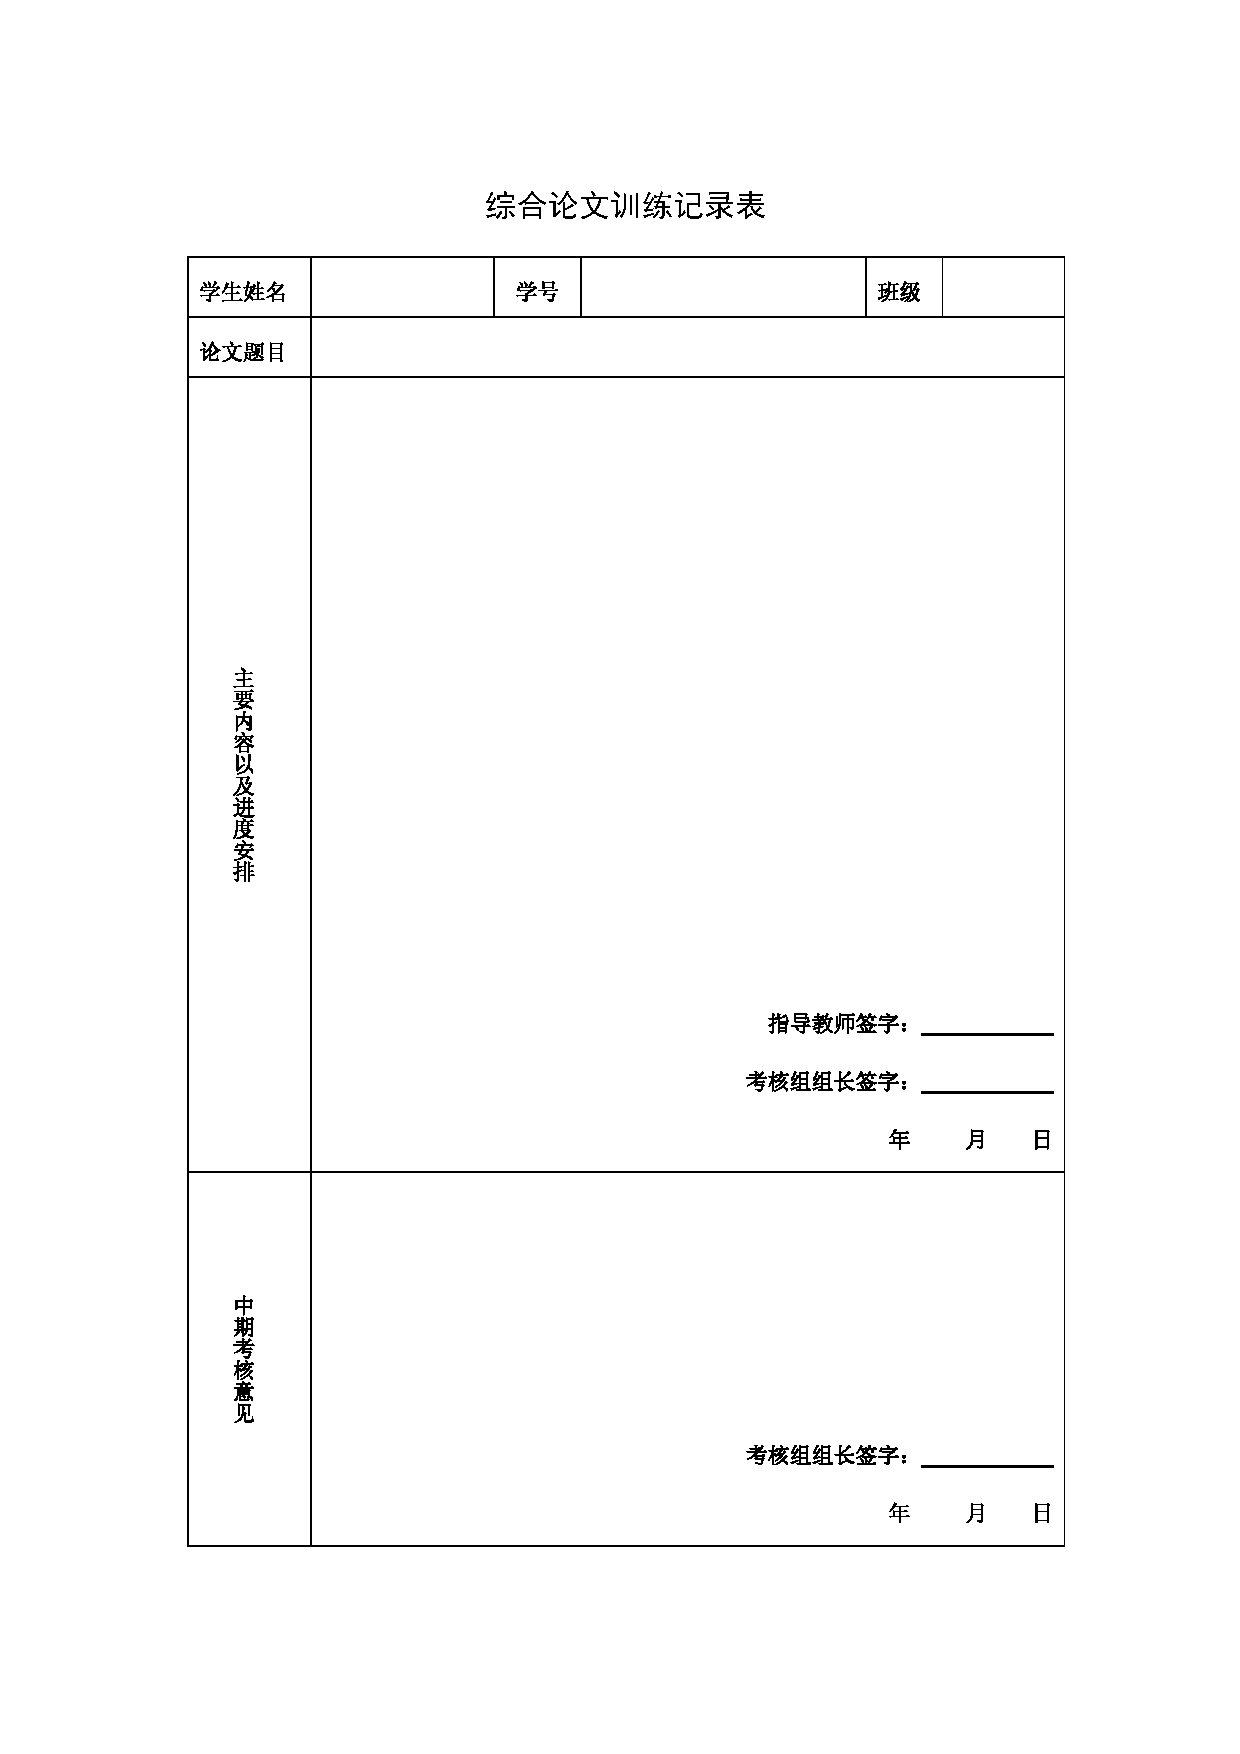
\includepdf[pages=-]{scan-record.pdf}
\end{document}
